\documentclass[12pt,twoside,letterpaper]{book}
%\usepackage{layout}
%\usepackage{makeidx}
\RequirePackage{verbatim}
%\RequirePackage{alltt}
\usepackage{ifpdf}
\usepackage{etoolbox}
\usepackage{multicol}
\usepackage{dsfont}
\usepackage{amsfonts}
\usepackage{amsmath}
\usepackage{array}
%\usepackage{wasysym}
\usepackage{qrcode}

\usepackage{amsmath, amssymb, array}
\usepackage{enumitem}
\usepackage{pgfplots}
\usepackage{graphicx}
\usepackage{lipsum}
\usepackage{stfloats}
\usepackage{multicol}
\setlength{\columnsep}{1cm}

\usepackage{minipage-marginpar}
\setlength{\columnsep}{1cm}
\usepackage{pinlabel} % for pin labels on figure


\newcommand{\boxcolor}{gray!30}
\usepackage{mdframed}
\newenvironment{boxme}{\begin{mdframed}[backgroundcolor=\boxcolor,linewidth=0pt,nobreak=true]}{\end{mdframed}}
\newenvironment{boxthm}{\begin{mdframed}[backgroundcolor=\boxcolor,nobreak=true]}{\end{mdframed}}
\newenvironment{boxdef}{\begin{mdframed}[backgroundcolor=\boxcolor,linewidth=0pt,nobreak=true]}{\end{mdframed}}


% Define a toggle that determines if a large or small print version
% will be printed.
\newtoggle{largePrint}
\toggletrue{largePrint}
\togglefalse{largePrint}

% Define a toggle that determines if solutions are printed. 
% (Not implemented yet)
\newtoggle{solutions}
\toggletrue{solutions}
\togglefalse{solutions}

\usepackage{graphicx}
\usepackage[pass]{geometry}
\usepackage{color}
\usepackage{hyperref}
\hypersetup{
  pdftitle={Recitation Activities for Math 1113, precalculus},
  pdfsubject={precalculus},
  pdfauthor={UGA Mathematics Department},
  pdfkeywords={classroom activities, precalculus},
  anchorcolor = {blue},
  colorlinks = {true},
  runcolor = {black},
  linkcolor = {red},
  urlcolor = {black},
  % pdfpagemode={FullScreen}
}

\usepackage{tikz}
\usepackage{pgf}
\usetikzlibrary{calc,mindmap,backgrounds,arrows,shapes.geometric}
%\usepackage{pstricks}


\pagestyle{myheadings}

%\setlength{\basicoddside}{\oddsidemargin}
%\setlength{\basicevenside}{\evensidemargin}
%\setlength{\basicwidth}{\textwidth}
%\setlength{\basictop}{\topmargin}
%\setlength{\basicheight}{\textheight}


\newcommand{\introduction}[1]{}

\font\tenit=cmti10
\makeatletter

\renewcommand{\@evenfoot}{\tenit University of Georgia Department of
  Mathematics\hfill}
\renewcommand{\@oddfoot}{\tenit \hfill Math 1113 - Precalculus}

\renewcommand{\section}{\@startsection
  {section}
  {1}
  {0em}
  {\baselineskip}
  {-1em}
  {\normalfont\normalsize\bfseries}}

\renewcommand{\subsection}{\@startsection
  {subsection}
  {2}
  {0em}
  {\baselineskip}
  {-1em}
  {\normalfont\normalsize\bfseries}}

\renewcommand{\subsubsection}{\@startsection
  {subsubsection}
  {2}
  {0em}
  {\baselineskip}
  {-2em}
  {\normalfont\normalsize\itshape}}

\makeatother


\newlength{\basicoddside}
\newlength{\basicevenside}
\newlength{\basicwidth}
\newlength{\basictop}
\newlength{\basicheight}

\setlength{\oddsidemargin}{0.15in}
\setlength{\evensidemargin}{0.15in}
\setlength{\textwidth}{6.0in}
\setlength{\topmargin}{-0.5in}
\setlength{\textheight}{9in}
\setlength{\marginparwidth}{52pt}


\newcommand{\activityParams}{
  %\setlength{\hoffset}{0in}
  %\setlength{\oddsidemargin}{-0.5in}
  %\setlength{\evensidemargin}{-0.5in}
  %\setlength{\textwidth}{7.5in}
  \setlength{\topmargin}{-0.5in}
  \setlength{\textheight}{9in}
}

\newcommand{\textParams}{
  \setlength{\oddsidemargin}{\basicoddside}
  \setlength{\evensidemargin}{\basicevenside}
  \setlength{\textwidth}{\basicwidth}
  \setlength{\topmargin}{\basictop}
  \setlength{\textheight}{\basicheight}
}



\newcommand{\sideNote}[1]{\marginpar{\tenit \raggedright #1}}
\newcommand{\doNotPrint}[1]{}


\newtheorem{lemma}{Lemma}[subsection]
\newtheorem{theorem}{Theorem}[subsection]



\newcounter{activity}
\setcounter{activity}{1}

\newcommand{\actTitle}[1]{
  \cleardoublepage
  \activityParams
  \stepcounter{activity}
  \markboth
  {Name: \hspace*{2.5in} \hfil  Video Activity: \theactivity}
  {Name: \hspace*{2.5in} \hfil  Video Activity: \theactivity}
  \stepcounter{section}
  \addcontentsline{toc}{section}{
    \protect\numberline{\thesection}{#1}}
}

\newcounter{hw}
\setcounter{hw}{0}
\newcommand{\hwTitle}[1]{
  \cleardoublepage
  \activityParams
  \stepcounter{hw}
  \markboth
  {Name: \hspace*{2.5in} \hfil  Home Work: \thehw}
  {Name: \hspace*{2.5in} \hfil  Home Work: \thehw}
  \stepcounter{subsubsection}
  \addcontentsline{toc}{subsubsection}{
    \protect\numberline{\thesubsubsection}{#1}}
}

\newcommand{\preClass}[1]{
  \cleardoublepage
  \activityParams
  \markboth
  {Name: \hspace*{2in} \hfil Preclass Work - Finish Before Class Begins \hfil}
  {Name: \hspace*{2in} \hfil Preclass Work - Finish Before Class Begins \hfil}
  \stepcounter{subsubsection}
  \addcontentsline{toc}{subsubsection}{
    \protect\numberline{\thesubsubsection}{#1}}
}

\newcommand{\postClass}{

  \cleardoublepage
  \activityParams
  \markboth
  {Name: \hspace*{2in} \hfil Postclass Work - Finish After Class \hfil}
  {Name: \hspace*{2in} \hfil Postclass Work - Finish After Class \hfil}
%  \stepcounter{subsubsection}
%  \addcontentsline{toc}{subsubsection}{
%    \protect\numberline{\thesubsubsection}{#1}}
}


\newcounter{quiz}
\setcounter{quiz}{1}
\newcommand{\qzTitle}[1]{
  \cleardoublepage
  \activityParams
  \stepcounter{quiz}
  \markboth
  {Name: \hspace*{2.5in} \hfil  #1 Quiz: \thequiz ~~~ }
  {Name: \hspace*{2.5in} \hfil  #1 Quiz: \thequiz ~~~ }
  \stepcounter{subsubsection}
  \addcontentsline{toc}{subsubsection}{
    \protect\numberline{\thesubsubsection}{#1}}
}

\newcounter{properties}
\setcounter{properties}{1}
\newcommand{\propertiesTitle}[1]{
  \cleardoublepage
  \activityParams
  \stepcounter{properties}
  \markboth
  {Name: \hspace*{2.5in} \hfil  #1 (Properties: \theproperties) ~ }
  {Name: \hspace*{2.5in} \hfil  #1 (Properties: \theproperties) ~ }
  \stepcounter{subsubsection}
  \addcontentsline{toc}{subsubsection}{
    \protect\numberline{\thesubsubsection}{#1}}
}


\newcommand{\stateSummary}{\item State and summarize two ideas from today's
  class. 
  \vfill 
  \centerline{\textit{(Over)}}
  \clearpage }


\newcommand{\addTOC}[1]{
  \stepcounter{section}
  \addcontentsline{toc}{section}{
    \protect\numberline{\thesection}{#1}}
  }



\newenvironment{problem}
{\begin{list}
{\arabic{enumi}.}
{\usecounter{enumi}
\setlength{\rightmargin}{0pt}
%\setlength{\rightmargin}{-72pt}
\setlength{\parsep}{0em}
\setlength{\listparindent}{0pt}
}}
{\end{list}}

\newenvironment{subproblem}
{\begin{list}
{(\alph{enumii})}
{\usecounter{enumii}
\setlength{\rightmargin}{0pt}
\setlength{\parsep}{1em}
\setlength{\listparindent}{0pt}
}}
{\end{list}}

\newenvironment{subsubproblem}
{\begin{list}
{(\roman{enumiii})}
{\usecounter{enumiii}
\setlength{\rightmargin}{0pt}
\setlength{\parsep}{1em}
\setlength{\listparindent}{0pt}
}}
{\end{list}}

\newenvironment{multiEqn}
{\begin{eqnarray*} 
 \begin{array}{rclclclcl}}
{\end{array}
 \end{eqnarray*}}


\setcounter{activity}{0}


% %%%%%%%%%%%%%%%%%%%%%%%%%%%%%%%%%%%%%%%%%%%%%%%%%%%%%%%%%%%%%%%%%%%%%%%
% List of definitions that are used in the different pages for the
% notes

% %%%%%%%%%%%%%%%%%%%%%%%%%%%%%%%%%%%%%%%%%%%%%%%%%%%%%%%%%%%%%%%%%%%%%%%
% Basic latex commands used throughout the notes.

\newcommand{\videoLink}[2]{%

  \noindent
  Watch the Pre-Class videos for #1 and answer the following
  questions. Remember that in your written work you are graded on the
  correctness of your supporting work and not just your final
  answer. Always give an exact answer unless you are explicitly told
  to round; calculator approximations will not receive full credit.

  \qrcode[height=2.0cm,hyperlink,tight]{#2}

  \bigskip

}

% Basic mathematical definitions used throughout the notes

\newcommand{\change}[1]{\triangle #1}
\newcommand{\fortyFive}{\frac{\sqrt{2}}{2}}
\newcommand{\imag}{j}
\newcommand{\half}{\mbox{$\frac{1}{2}$}}
\newcommand{\deltat}{\mbox{$\triangle t$}}
\newcommand{\deltax}{\mbox{$\triangle x$}}
\newcommand{\deltay}{\mbox{$\triangle y$}}

\newcommand{\deriv}[2]{\frac{d}{d#2}#1}
\newcommand{\derivTwo}[2]{\frac{d^2}{d#2^2}#1}

\newcommand{\lp}{\left(}
\newcommand{\rp}{\right)}


% %%%%%%%%%%%%%%%%%%%%%%%%%%%%%%%%%%%%%%%%%%%%%%%%%%%%%%%%%%%%%%%%%%%%%%
% trigonometry definitions
\newcommand{\trigTriangle}[5]{%
	\begin{tikzpicture}[scale=2.5]
	\draw (0,0) -- (2,0) -- (2,1) -- (0,0);
	\draw (1.9,0) -- (1.9,0.1) -- (2,0.1);
	\draw (0.3,0) arc(0:40:0.2);
	\draw (0.5,0.1) node { #1 };
	\draw (1.8,0.7) node { #2 };
	\draw (1,-0.1) node { #3 };
	\draw (1,0.6) node { #4 };
	\draw (2,0.8) arc(270:210:0.2);
	\draw (2.1,0.5) node { #5 };
	\end{tikzpicture}
}


% %%%%%%%%%%%%%%%%%%%%%%%%%%%%%%%%%%%%%%%%%%%%%%%%%%%%%%%%%%%%%%%%%%%%%%
% Basic linear algebra commands

\newcommand{\arrayTwo}[4]{
  \left[
  \begin{array}{rr}
    #1 & #2 \\
    #3 & #4
  \end{array}
  \right]
}

\newcommand{\vecTwo}[2]{
  \left[
  \begin{array}{r}
    #1 \\  #2
  \end{array}
  \right]
}

\newcommand{\vecFour}[4]{
  \left[
  \begin{array}{r}
    #1 \\  #2 \\ #3 \\ #4
  \end{array}
  \right]
}


\newcommand{\stateTwo}[2]{
  \begin{array}{rr}
    \mbox{\fontsize{6}{6}\selectfont $#1$} \\  \mbox{\fontsize{6}{6}\selectfont $#2$}
  \end{array}
}


\newcommand{\arrayThree}[9]{
  \left[
    \begin{array}{rrr}
      #1 & #2 & #3 \\
      #4 & #5 & #6 \\
      #7 & #8 & #9
    \end{array}
  \right]
}

\newcommand{\startRowOps}{
  \left[
    \begin{array}{rrr|r}
}

\newcommand{\oneRowOps}[4] {
      #1 & #2 & #3 & #4 \\
}

\newcommand{\stopRowOps}{
    \end{array}
  \right]
}


\newcommand{\vecThree}[3]{
  \left[
  \begin{array}{r}
    #1 \\  #2 \\ #3
  \end{array}
  \right]
}


\newcommand{\stateThree}[3]{
  \begin{array}{r}
    \mbox{\fontsize{6}{6}\selectfont $#1$} \\  
    \mbox{\fontsize{6}{6}\selectfont $#2$} \\ 
    \mbox{\fontsize{6}{6}\selectfont $#3$}
  \end{array}
}





\newcommand{\detTwo}[4]{
  \left|
  \begin{array}{rr}
    #1 & #2 \\
    #3 & #4
  \end{array}
  \right|
}



\newcommand{\detThree}[9]{
  \left|
    \begin{array}{rrr}
      #1 & #2 & #3 \\
      #4 & #5 & #6 \\
      #7 & #8 & #9
    \end{array}
  \right|
}




\newcommand{\startRowFour}{
  \left[
    \begin{array}{rrrr}
}

\newcommand{\oneRowFour}[4] {
      #1 & #2 & #3 & #4 \\
}




\newcommand{\startRowOpsTwo}{
  \left[
    \begin{array}{rr|rr}
}

\newcommand{\oneRowOpsTwo}[4] {
      #1 & #2 & #3 & #4 \\
}


\newcommand{\startRowOpsThree}{
  \left[
    \begin{array}{rrr|rrr}
}

\newcommand{\oneRowOpsThree}[6] {
      #1 & #2 & #3 & #4 & #5 & #6 \\
}





%%% Local Variables: 
%%% mode: latex
%%% TeX-master: t
%%% End: 

\includeonly{2.2}

\begin{document}

\iftoggle{largePrint}{\fontsize{2cm}{1cm}\selectfont}

\title{Video Workbook \\
  Math 1113 - Precalculus
  \iftoggle{solutions}{%
    \\\textit{Solution Manual}
  }
}
\author{University of Georgia\\Department of Mathematics}

\date{}
\maketitle

\noindent
Copyright (C)  2017-2023 Toyin Alli and Kelly Black University of Georgia Department of Mathematics

\noindent
Permission is granted to copy, distribute and/or modify this document
under the terms of the GNU Free Documentation License, Version 1.3
or any later version published by the Free Software Foundation;
with no Invariant Sections, no Front-Cover Texts, and no Back-Cover Texts.
A copy of the license is included in the section entitled "GNU
Free Documentation License".

\vfill

\qrcode[height=3.0cm,hyperlink,tight]{https://github.com/KellyBlack/Precalculus}


\tableofcontents

\clearpage


\chapter{Functions and Preliminaries}

 
\actTitle{1.1 - Rectangular Coordinate System}

\videoLink{Section 1.1}{https://www.youtube.com/playlist?list=PLYHZK3b8UFw3ad1wlhTMGcL5kgita6QGS}

\noindent \textbf{Topics:}  $x,y$-plane and coordinate system, quadrants, plotting points, distance formula\\

\noindent \textbf{Student Learning Outcomes:}
\begin{enumerate}
\item Students will be able to plot points in an $x,y$-plane using a coordinate system.
\item Students will be able to determine the distance between two
  points on an $x,y$-plane using the distance formula.
\end{enumerate}

\hrule 
\subsection{Rectangular Coordinate System}

\begin{center}
  \begin{tikzpicture}
    \begin{axis}[
      xmin=-5, xmax=5,
      ymin=-5, ymax=5,
      axis lines=center,
      axis on top=true,
      domain=0:1,
      ]
    \end{axis}
  \end{tikzpicture}
\end{center}


\begin{enumerate}
\item First, label the $x$ and $y$ axes on the rectangular coordinate system below.  Then plot and label the given points.\\

$$A(2,-3) \quad \quad B(-2,0) \quad \quad C(-1,2)$$
\begin{center}
\begin{tikzpicture}
\begin{axis}[
    xmin=-5, xmax=5,
    ymin=-5, ymax=5,
    axis lines=center,
    axis on top=true,
    domain=0:1,
    ]

   
\end{axis}
\end{tikzpicture}
\end{center}
\end{enumerate}


\newpage


\subsection{The Distance Formula}
\noindent We have just completed an activity called Crowd Crumple.  You should now have a piece of paper with a graph, two labeled points, and a line connecting those two points labeled $d$.
\begin{enumerate}
\item Use prior knowledge to find the distance between the two points on your paper or make a reasonable guess and write your answer below.\\[.5in]

\item Determine the horizontal and vertical distances between your two points.
\begin{enumerate}
\item Determine the \textbf{horizontal distance} between your points $(x_1,y_1)$ and $(x_2,y_2)$:\\
(This is the distance between the $x$-values.)\\[.5in]
\item Determine the \textbf{vertical distance} between your points $(x_1,y_1)$ and $(x_2,y_2)$:\\
(This is the distance between the $y$-values.)\\[.5in]
\item Draw lines on your graph to represent the horizontal and vertical distances between your two points.  Do your lines form a recognizable shape?\\[.5in]
\item How can we use these two values to determine the straight-line distance $d$ between your points $(x_1,y_1)$ and $(x_2,y_2)$?\\[.5in]
\item Calculate the distance between your points $(x_1,y_1)$ and $(x_2,y_2)$.

\end{enumerate}
\vfill


\newpage


\noindent \textbf{The Distance Formula:}  The distance between points $(x_1,y_1$ and $(x_2,y_2)$ is given by $d=$

\vfill
\item Use the distance formula to calculate the distance between the points $(1,5)$ and $(4,9)$.
\end{enumerate}
\vfill
\vfill
\vfill
\subsection{Student Learning Outcomes Check}

\begin{enumerate}
\item Can you plot points in an $x,y$-plane using a coordinate system?\\
\item Are you able to determine the distance between two points on an $x,y$-plane using the distance formula?\\
\end{enumerate}

\noindent \textbf{If any of your answers were no, please ask about these topics in class.}




\actTitle{1.1 - Rectangular Coordinate System}

\videoLink{Section 1.1}{https://www.youtube.com/playlist?list=PLYHZK3b8UFw3ad1wlhTMGcL5kgita6QGS}

\noindent \textbf{Topics:}  $x,y$-plane and coordinate system, quadrants, plotting points, distance formula, graphing an equation, $x$ and $y$ intercepts\\

\noindent \textbf{Student Learning Outcomes:}
\begin{enumerate}
\item Students will be able to plot points in an $x,y$-plane using a coordinate system.
\item Students will be able to determine the distance between two points on an $x,y$-plane using the distances formula.
\item Students will be able to graph an equation on an $x,y$-plane and determine the $x$ and $y$ intercepts of the equation.
\end{enumerate}

\hrule
\bigskip

\noindent \textbf{Rectangular Coordinate System}\\

\begin{enumerate}
\item Plot and label the given points on the coordinate axes below.\\

$$A(2,-3) \quad \quad B(-2,0) \quad \quad C(-1,2)$$
\begin{center}
\begin{tikzpicture}
\begin{axis}[
    xmin=-5, xmax=5,
    ymin=-5, ymax=5,
    axis lines=center,
    axis on top=true,
    domain=0:1,
    ]

   
\end{axis}
\end{tikzpicture}
\end{center}

\clearpage

\noindent \textbf{The Distance Formula}\\
\item Label the points $(1,5)$ and $(4,9)$ on the graph below.  Then draw a line representing the distance between the points and label that line $d$.

\begin{center}

\begin{tikzpicture}
\begin{axis}[
    xmin=-2, xmax=6,
    ymin=-2, ymax=10,
    axis lines=center,
    axis on top=true,
    domain=1:4,
    ]

\end{axis}

\end{tikzpicture}
\end{center}

\begin{enumerate}
\item Determine the horizontal distance between the points $(1,5)$ and $(4,9)$:\\
(This is the distance between the $x$-values.)\\[.3in]
\item Determine the vertical distance between the points $(1,5)$ and $(4,9)$:\\
(This is the distance between the $y$-values.)\\[.3in]
\item How can we use these two values to determine the straight-line distance $d$ between the points $(1,5)$ and $(4,9)$?\\[.3in]
\item Calculate the distance between the points $(1,5)$ and $(4,9)$.

\end{enumerate}
\vfill

\noindent \textbf{The Distance Formula:}  The distance between points $(x_1,y_1$ and $(x_2,y_2)$ is given by $$d=\sqrt{(x_2-x_1)^2+(y_2-y_1)^2}$$

\clearpage

\noindent \textbf{Graph Equations by Plotting Points}\\
\item Graph the equation $y=x+2$.\\
\begin{center}
\begin{tikzpicture}
\begin{axis}[
    xmin=-5, xmax=5,
    ymin=-5, ymax=5,
    axis lines=center,
    axis on top=true,
    domain=0:1,
    ]

   
\end{axis}
\end{tikzpicture}
\end{center}

\item Graph the equation $y-|x|=-1$.
\begin{center}
\begin{tikzpicture}
\begin{axis}[
    xmin=-5, xmax=5,
    ymin=-5, ymax=5,
    axis lines=center,
    axis on top=true,
    domain=0:1,
    ]

   
\end{axis}
\end{tikzpicture}
\end{center}


\noindent \textbf{Finding $x$ and $y$ Intercepts}\\
An $x$-intercept is a point $(x,y)$ where a graph crosses the $x$-axis and a $y$-intercept is a point $(x,y)$ where a graph crosses the $y$-axis.\\

\item Determine the $x$-intercept(s) and $y$-intercepts of the previous example, $y-|x|=-1$ and label them on the graph.
\begin{enumerate}
\item $x$-intercept(s):\\
$y$-intercept(s):\\
\item What do you notice about the intercepts?\\
\item How are they different?
\end{enumerate}
\clearpage

\item Determine the $x$-intercepts of $y-|x|=-1$ algebraically.
\vfill
\item Determine the $y$-intercept of $y-|x|=-1$ algebraically.
\vfill
\end{enumerate}

\noindent \textbf{Student Learning Outcomes Check}

\begin{enumerate}
\item Can you plot points in an $x,y$-plane using a coordinate system?\\
\item Are you able to determine the distance between two points on an $x,y$-plane using the distances formula?\\
\item Can you graph an equation on an $x,y$-plane and determine the $x$ and $y$ intercepts of the equation?
\end{enumerate}

\noindent \textbf{If any of your answers were no, please ask about these topics in class.}



\actTitle{1.3 - Functions and Relations}

\videoLink{Section 1.3}{https://www.youtube.com/playlist?list=PLYHZK3b8UFw1_K7VRAlYGdUZOaqjJTOZ\_}

\noindent \textbf{Topics:}  relation, function, function notation, $x$ and $y$-intercepts of a function, domain and range of a function, graph of a function, characteristics of functions\\

\noindent \textbf{Student Learning Outcomes:}
\begin{enumerate}
\item Students will be able to determine whether a relation is a function.
\item Students will be able to recognize and apply function notation.
\item Students will be able to determine function characteristics including domain, range, increasing, decreasing, and constant.
\end{enumerate}

\hrule 

\bigskip

\subsection{Determine whether a relation is a function}
In mathematics, we can express the relationship between two values as a set of ordered pairs.
\begin{itemize}
\item The cost of mailing a package is related to the weight of a package.
\item The minimum braking distance of a car depends on the speed of the car.
\item The test score that a student earns is related to the number of hours of study.\\
\end{itemize}

\noindent \textbf{The Definition of a Relation:}  A set of ordered pairs $(x,y)$ is called a \textbf{relation} in $x$ and $y$.
\begin{itemize}
\item The set of $x$ values in the ordered pair is called the \textbf{domain} of the relation.
\item The set of $y$ values in the ordered pair is called the \textbf{range} of the relation.\\
\end{itemize}


\begin{enumerate}
\item Determine the domain and range of the following relations.
\begin{enumerate}
\item $\{(8,92), (3,58), (11,98), (5,72), (8,86) \}$\\[1in]
\item $\{(3,1), (2,5), (-4,2), (-1,1), (4,-4) \}$\\[1in]
\end{enumerate}
\vfill
Only one of the previous relations are functions.\\

\newpage

\noindent \textbf{The Definition of a Function:}  Given a relation in $x$ and $y$, we say that \textbf{$y$ is a function of $x$} if for each value of $x$ in the domain, there is exactly one value of $y$ in the range.\\

For our purposes, a \emph{function} is something (like an abstract machine) that takes in numbers and gives numbers back.  For each number that goes into the machine, you get a number back.



 \subsection{Examples of functions and function notation}
Examples of functions include: $f(x) = 3x^2 +7$,\quad  $y = \dfrac{x^3+x+6}{7-x^4}$, and $g(t) = \sin(t)$\\[.5in]




\item If $f(x)= 7 - 2x - x^2$, determine $f(-1)$. \\[.5in]

\item If $a$ is a positive real number, determine the following values for the function $f(x) = \dfrac{x}{5-x}$.

\begin{enumerate}

\item $f(\sqrt{a}+2)$ \\[.5in]

\item $f(\sqrt{a})+f(2)$ \\[.5in]


\item $f(a^2+1)+3$ \\[.5in]
\end{enumerate}




\item Let $f(x)$ be defined on the real numbers as follows.
\begin{itemize}
\item Start with a number $x$.
\item Square $x$ and subtract it from 3 more than what you started with.
\item Divide the result by one more than the square root of the original.
\item Square the result and add the number you started with.
\end{itemize}

Write a formula for $f(x)$. \\

\newpage

\noindent \begin{tabular}{| l |} \hline A graph is the graph of a function if it passes the \emph{vertical line test}, meaning that every vertical\\ line intersects the graph in at most one point. \\ \hline
\end{tabular}

\subsection{Characteristics of a Function}
\vspace{-.1in} 
\item Using the graph of the function $g$ below, determine the following. \\
\begin{tabular}{l l } \begin{tabular}{l} \scalebox{0.3}{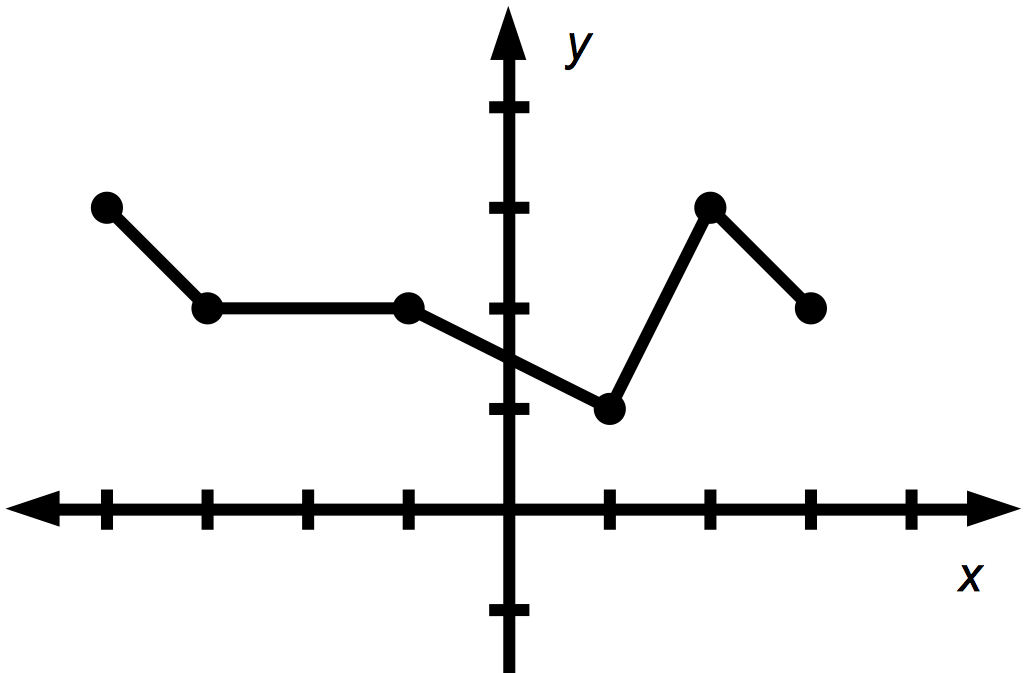
\includegraphics{pwgraph}} \end{tabular} &

\begin{tabular}{l }
 $g(-4)$ \\ \\
 $g(-2)$ \\ \\
 all $x$ such that $g(x)=3$ \\ \\
 all $x$ such that $g(x)<2$ \\[1.5in]
\end{tabular}
\end{tabular}




\noindent \begin{tabular}{| l | }
\hline The \emph{domain} is the collection of all the numbers that go \emph{into} the function. When no domain \hfill \\is specified, the domain is the collection of all the numbers that make sense when you plug \\ them into the function. \\ \hline
\end{tabular}\\[.3in]

\noindent \begin{tabular}{| l | }
\hline The \emph{range} is the collection of all the numbers that \emph{come out of} the function. 
\\ \hline
\end{tabular}\\[.3in]
\item Determine the domain and range of the function $g(x)$ in the previous example. Then determine intervals where $g(x)$ is increasing, decreasing, or constant.\\[1in]


\newpage

\item Determine the domain of each of the following functions. Give your answer in interval notation.

\vspace{-.1in}
$$g(x) = -x^3 + 7x^2 + 17 \quad \quad \quad \quad \quad \quad f(x)=\sqrt{4x+5} \quad \quad  \quad \quad h(x)=\dfrac{1}{x^2-14}$$
\vfill



\end{enumerate}

\noindent \textbf{Student Learning Outcomes Check}

\begin{enumerate}
\item Can you determine whether a relation is a function?
\item Are you able to recognize and apply function notation?
\item Can you determine function characteristics including domain, range, increasing, decreasing, and constant?
\end{enumerate}

\noindent \textbf{If any of your answers were no, please ask about these topics in class.}



\actTitle{1.4 - Lines}

\noindent \textbf{Topics:}  Equations of lines, parallel and perpendicular lines, linear models, average rate of change\\

\noindent \textbf{Student Learning Outcomes:}
\begin{enumerate}
\item Students will be able to graph linear equations.
\item Students will be able to determine the slope of a line and apply the slope-intercept form of a line.
\item Students will be able to compute the average rate of change of a function.
\end{enumerate}

\hrule 

\bigskip

\subsection{Slope of a Line} ~

\noindent 
\begin{tabular}{| l |} \hline
The \underline{slope of a line} is $m = \dfrac{y_2-y_1}{x_2-x_1}$.  \\ \hline
 \end{tabular} 
 



\begin{enumerate}
\item Sketch the line through the pair of points $P(4,2)$ and $Q(-3,5 )$, and find the slope of the line. \\
\scalebox{0.3}{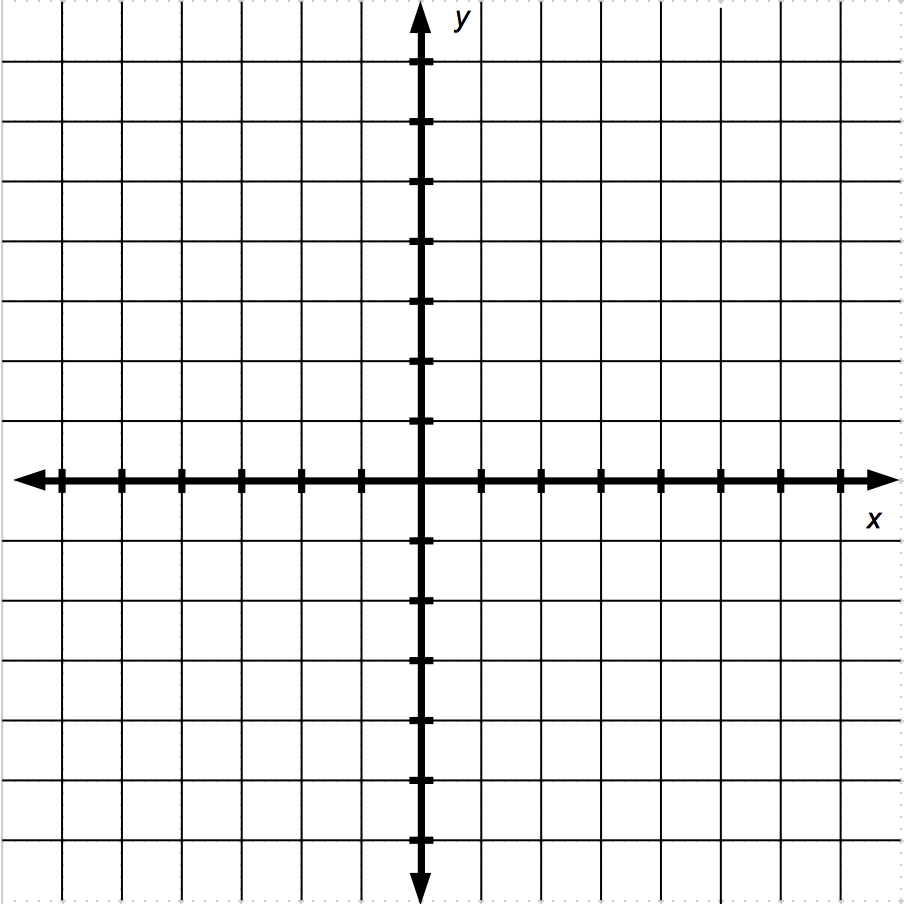
\includegraphics{bigaxes}} 

\hspace{-.3in} \begin{tabular}{| l |}\hline
 \noindent The \underline{point-slope equation} for the line through the point $(x_1,y_1)$ with slope $m$ is \\

 $y-y_1 = m(x-x_1)$. \\ \hline
\end{tabular} 

\vspace{-.1in}
\item Determine a \emph{point-slope} equation for the line through $P(4,2)$ and $Q(-3,5)$.(See above.)\\[1in]






\hspace{-.3in} \begin{tabular}{| l |}\hline The \underline{slope-intercept equation} for the line with slope $m$ and $y$-intercept $b$ is \\

 $y = mx +b$. \\ \hline
\end{tabular} 



\vspace{-.1in}
\item Determine the \emph{slope-intercept} equation for the line through $(3, -2)$ which has slope $-4$. \\[1in]



\noindent \textbf{Horizontal lines} have 0 slope and \textbf{vertical lines} have undefined slopes.\\[1in]


\subsection{Parallel and Perpendicular Lines} ~

\hspace{-.3in} \begin{tabular}{| l |  }
\hline Parallel lines have the \emph{same slope.} \\ \hline
\end{tabular} %\\[.5in]

\vspace{-.1in}
\item Determine a point-slope equation for the line through $(-1,2)$ which is parallel to the line $2x + 3y - 5 = 0$ and graph the equation.\\
\scalebox{0.3}{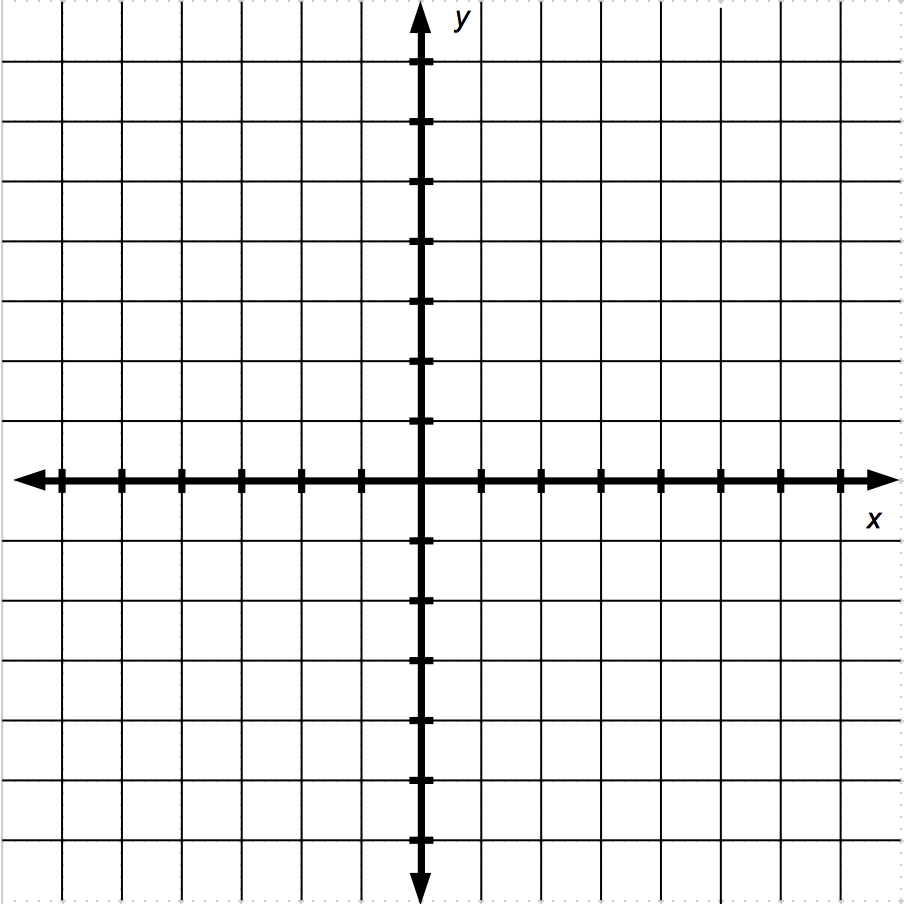
\includegraphics{bigaxes}} 
\\[1in]





\hspace{-.3in}\begin{tabular}{| l |  }
\hline Perpendicular lines have slopes that are ``negative reciprocals" of each other. If $m_1$ is the \\ slope of one of the lines, then the slope of the other line must be $-1/m_1$. \\ \hline
\end{tabular} 

\item Determine an equation of the line through the point $(-3, 1)$ which is perpendicular to the line $2x+4y+7=0$ and graph the equation.\\
\scalebox{0.3}{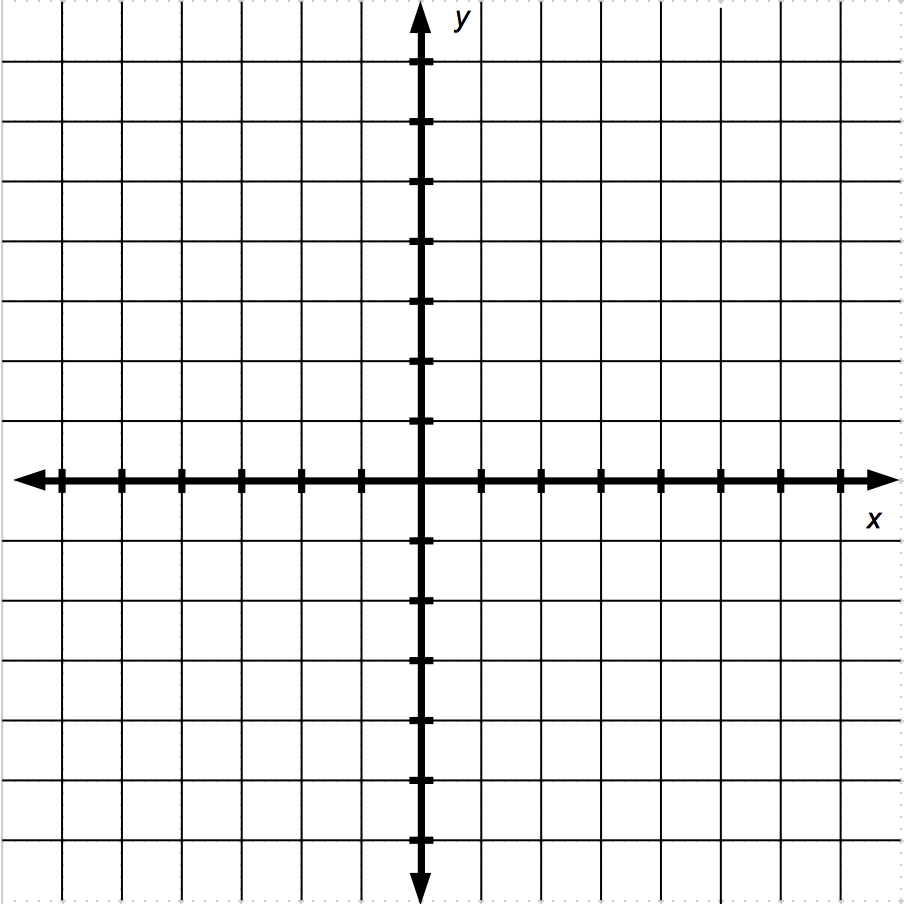
\includegraphics{bigaxes}} 
\\


\subsection{Average Rate of Change}
\textbf{Average Rate of Change}\\
Given any function $y=f(x)$, we calculate the average rate of change of $y$ with respect to $x$ over the interval  $[x_1,x_2]$ by dividing the change in value of $y$, $\Delta y=f(x_2)-f(x_1)$, by the length  $\Delta x=x_2-x_1$ of the interval over which the change occurs.\\


 The \textbf{\emph{average rate of change}} of $y=f(x)$ with respect to $x$ over the interval $[x_1,x_2]$ is
 $$\frac{\Delta y}{\Delta x}=\frac{y_2-y_1}{x_2-x_1}=\frac{f(x_2)-f(x_1)}{x_2-x_1}$$\\ 
 
\noindent \textbf{Note:  }An average rate of change needs two points (or endpoints on an interval). 






\item Given the function defined $f(x)=x^2-1$, determine the average rate of change from $x_1=-2$ to $x_2=0.$\\[2in]


\end{enumerate}

\noindent \textbf{Student Learning Outcomes Check}

\begin{enumerate}
\item Can you graph a linear equation?
\item Can you determine the slope of a line and apply the slope-intercept form of a line?
\item Can you compute the average rate of change of a function?
\end{enumerate}

\noindent \textbf{If any of your answers were no, please ask about these topics in class.}


\actTitle{1.5 - Modeling with Linear Equations}



\noindent \textbf{Topics:}  linear relationship, interpretation of the point-slope formula, and constructing a linear equation\\

\noindent \textbf{Student Learning Outcomes:}
\begin{enumerate}
\item Students will be able to apply the point-slope formula.
\item Students will be able to construct a linear equation from a written description.

\end{enumerate}

\hrule 

\bigskip

\subsection{Applying the Point-Slope Formula} ~

\begin{tabular}{| l |}\hline
The \underline{point-slope equation} for the line through the point $(x_1,y_1)$ with slope $m$ is \\

 $y-y_1 = m(x-x_1)$. \\ \hline
\end{tabular} 

\vspace{-.1in}
\begin{enumerate}
\item Use the point-slope formula to find an equation of the line passing through the point $(2,-3)$ and having slope -4.  Write your answer in slope-intercept form.\\[1.5in]









\item Use the point-slope formula to write an equation of the line passing through the points $(4,-6)$ and $(-1,2)$.  Write your answer in slope-intercept form.\\[3in]



\newpage


\subsection{Create Linear Functions to Model Data}
\noindent In many day-to-day applications, two variables are related linearly.  This means that any given any change in an independent variable, $x$, will always produce a corresponding change in the dependent variable, $y$.  And when you plot this relationship on a graph, it traces a straight line.\\

\item A family plan for a cell phone has a monthly base price of \$99 plus \$12.99 for each additional family member added beyond the primary account holder.
\begin{enumerate}
\item Write a linear function to model the monthly cost $C(x)$, in dollars, of a family plan for $x$ additional family members added.\\[1in]
\item Evaluate $C(4)$ and interpret the meaning in the context of this problem.\\[1in]
\end{enumerate}




\item The data given in the table represent the age and systolic blood pressure for a sample of 12 randomly selected healthy adults.\\
\begin{table}[h]
\centering

\begin{tabular}{|l|l|}
\hline
Age in years & Pressure in mmHG \\ \hline
17           & 110              \\ \hline
21           & 118              \\ \hline
26           & 120              \\ \hline
32           & 121              \\ \hline
35           & 115              \\ \hline
37           & 124              \\ \hline
43           & 126              \\ \hline
51           & 130              \\ \hline
58           & 132              \\ \hline
59           & 139              \\ \hline
65           & 137              \\ \hline
68           & 141              \\ \hline
\end{tabular}
\end{table}

\newpage
\begin{enumerate}
\item Suppose $x$ represents the age of an adult, in years, and $y$ represents the systolic blood pressure, in mmHG.  Use the points $(21, 118)$ and $(51, 130)$ to write a linear model relating $y$ as a function of $x$.\\[2.5in]
\item Interpret the meaning of the slope in the context of this problem.\\[.5in]
\item Use the model to estimate the systolic blood pressure for a 55 year old.  Round to the nearest whole unit.\\[2in]
\end{enumerate}



\end{enumerate}

\noindent \textbf{Student Learning Outcomes Check}

\begin{enumerate}
\item Can you interpret the point-slope formula?
\item Are you able to construct a linear equation from a written description?
\end{enumerate}

\noindent \textbf{If any of your answers were no, please ask about these topics in class.}


\actTitle{1.6 - Transfomations of Graphs}

\noindent \textbf{Topics:}  basic functions, vertical translations and scaling, horizontal translations and scaling, horizontal and vertical reflections, graphing transformations\\

\noindent \textbf{Student Learning Outcomes:}
\begin{enumerate}
\item (In class) Students will be able to recognize basic functions.
\item Students will be able to transform graphs of functions.
\item Students will be able to graph a function based on transformations.
\end{enumerate}

\hrule 

\bigskip


\subsection{Vertical and Horizontal Shifts} ~

\hspace{-.4in} \begin{tabular}{| l |} \hline \underline{Vertical shifts.} Assume that $c$ is a positive number. \\
The graph of $y = f(x)+c$ is obtained from the graph of $y=f(x)$ by shifting it $c$ units upward. \\
The graph of $y = f(x)-c$ is obtained from the graph of $y=f(x)$ by shifting it $c$ units downward.
 \\ \hline
\end{tabular}

\begin{enumerate}

\item For this problem, let $f(x)=x^2$. Sketch the graph of the function $y=f(x) - 3$. Compare the domains and ranges of $y=f(x)$ and $y=f(x)-3$.



\scalebox{0.4}{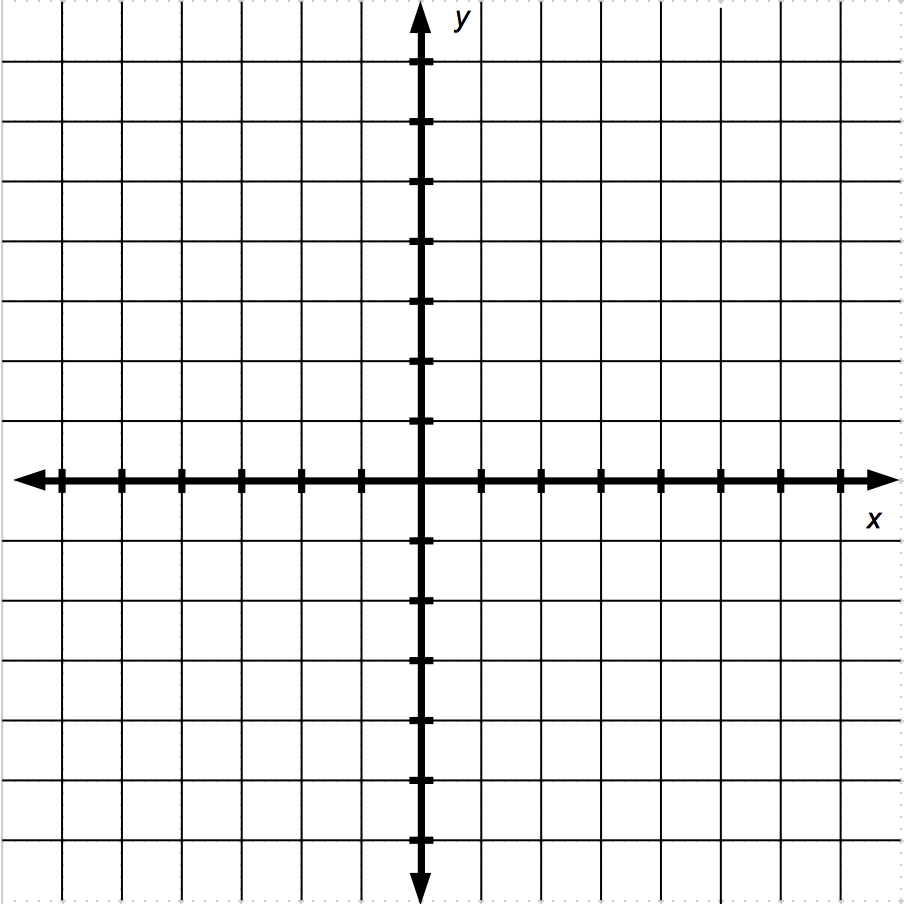
\includegraphics{bigaxes}} 


\newpage
\hspace{-.4in} \begin{tabular}{| l |} \hline \underline{Horizontal shifts.} Assume that $c$ is a positive number. \\
The graph of $y = f(x-c)$ is obtained from the graph of $y=f(x)$ by shifting it $c$ units to the right. \\
The graph of $y = f(x+c)$ is obtained from the graph of $y=f(x)$ by shifting it $c$ units to the left.
 \\ \hline
\end{tabular} 

\item Convince yourself that the rule above is correct by using the example $f(x)=x^2.$ Sketch the graph of $y = f(x -2)$ on the axes below.  \\
\scalebox{0.4}{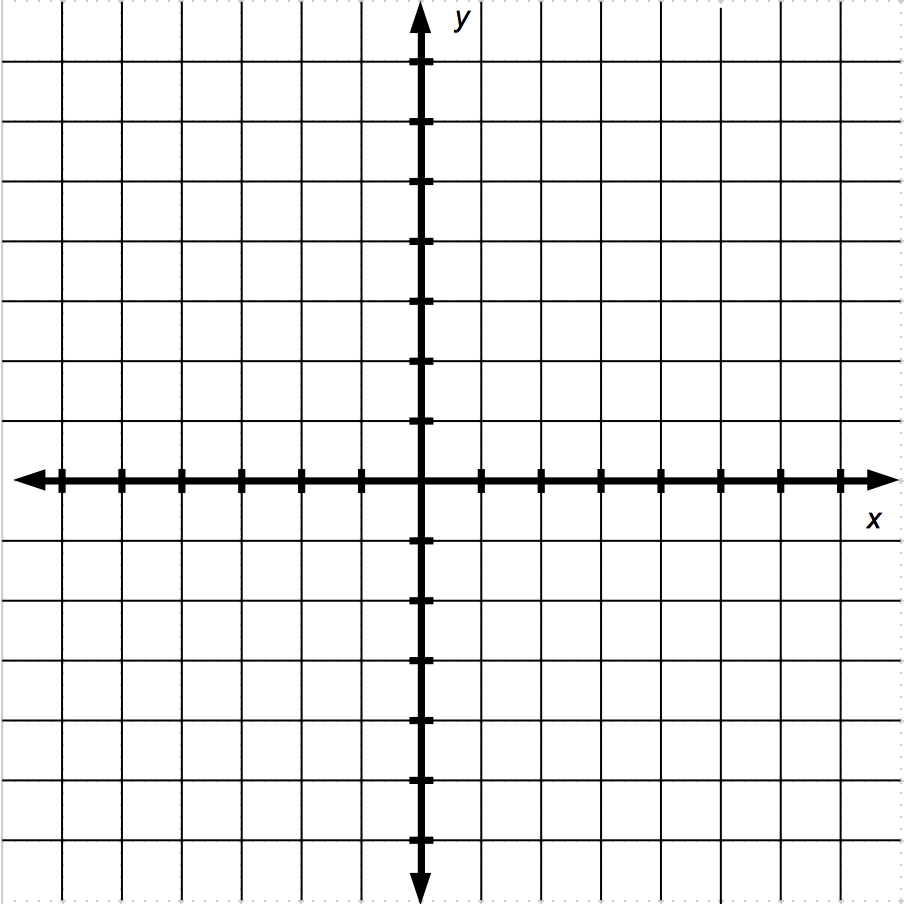
\includegraphics{bigaxes}} \\[1in]

\item Compare the domains and ranges of $y = \sqrt{x}$ and $f(x)=\sqrt{x+4}$. Think about why this makes sense and is consistent with the shifting.\\[2in]



\item If the point $(3, -4)$ is on the graph of $y = f(x)$, find the corresponding point on the graph of $y = f(x - 5)+3$. \\

\newpage

\subsection{Reflection, Compression, and Stretching} ~

\hspace{-.4in} \begin{tabular}{| l |} \hline \underline{Reflection through the $x$-axis.} The graph of $y=-f(x)$ is obtained by reflecting the graph of $y=f(x)$ \\ through the $x$-axis.
 \\ \hline
\end{tabular} 


\vspace{-.1in}
\item For the graph of $y=f(x)$ shown below, sketch the graph of $y=-f(x)$.\\
\scalebox{0.5}{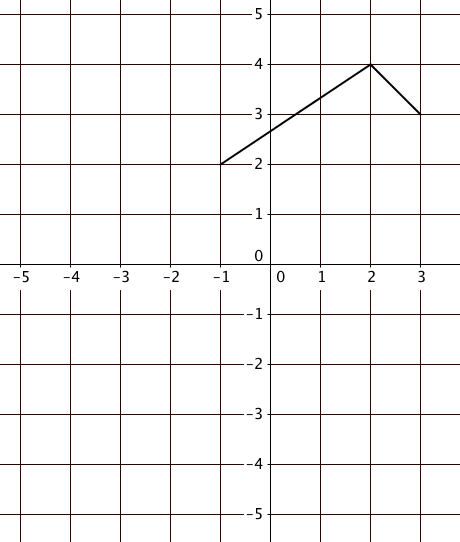
\includegraphics{pwshift1}} 




\hspace{-.3in} \begin{tabular}{| l |} \hline \underline{Vertical Compression/Stretching} Assume that $c$ is a positive number. \\
If $c>1$, the graph of $y=cf(x)$ is obtained by stretching the graph of $y=f(x)$ vertically \\ by a factor of $c$. \\
If $c$ is between $0$ and $1$, the graph of $y=cf(x)$ is obtained by compressing the graph vertically\\ by a factor of $1/c$.
 \\ \hline
\end{tabular} 


\vspace{-.1in}
\item If the point $P(3,-1)$ is on the graph of $y=f(x)$, find the corresponding point on the graph of (a) $y = 7f(x)$ and (b) $y = \dfrac{1}{4}f(x)$. \\[.4in]



\newpage
\item For the graph of $y=f(x)$ shown below, sketch the graph of $y=2f(x+3)-1$. \\
%\noindent Hint: work in stages, one modification at a time. Use order of operations to make your stages.\\
\scalebox{0.25}{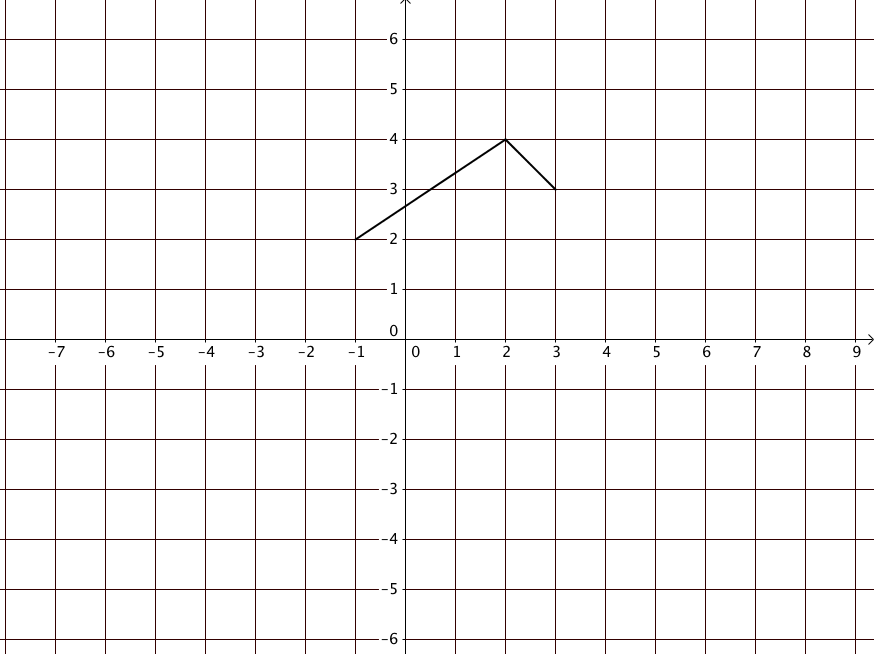
\includegraphics{pwshift}} 
%\end{enumerate}
%
%
%
%
%\noindent MATH 1113 - Alli  \hfill Section 2.5 - Graphs of Functions\\
%\noindent Part 2 \\
%\noindent Topics: reflections of graphs, stretching/compressing of graphs   \\



\begin{tabular}{| l |} \hline \underline{Reflection through the $y$-axis.} The graph of $y=f(-x)$ is obtained by reflecting the graph of $y=f(x)$ \\ through the $y$-axis.
 \\ \hline
\end{tabular} 

%\begin{enumerate}
\vspace{-.1in}
\item For the graph of $y=f(x)$ shown below, sketch the graph of $y=f(-x)$.\\
\scalebox{0.5}{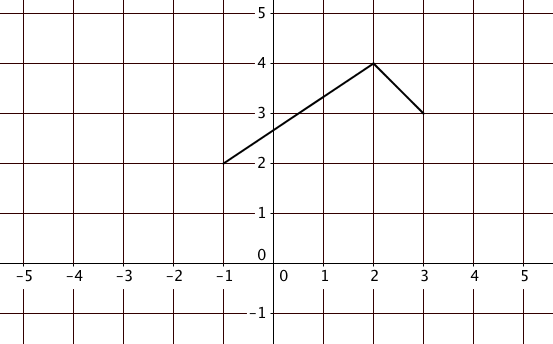
\includegraphics{pwshift4}} 






\hspace{-.4in} \begin{tabular}{| l |} \hline \underline{Horizontal Compression/Stretching} Assume that $c$ is a positive number. \\
If $c>1$, the graph of $y=f(cx)$ is obtained by compressing the graph horizontally by a factor $c$. \\
If $c$ is between $0$ and $1$, the graph of $y=f(cx)$ is obtained by stretching the graph of $y=f(x)$ \\ horizontally by a factor of $1/c$.
 \\ \hline
\end{tabular} 

\vspace{-.1in}
\item For the graph of $y=f(x)$ shown below, sketch the graph of $y=f(2x)$.\\
\scalebox{0.3}{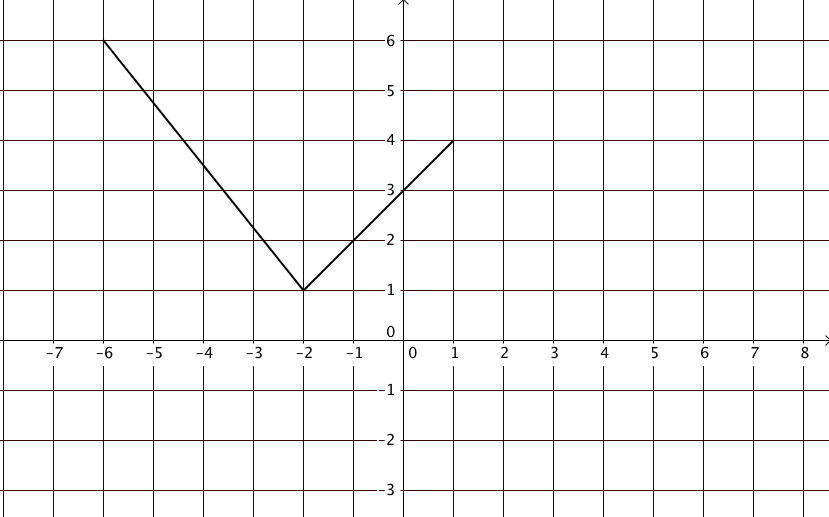
\includegraphics{pwshift2}} 

\newpage
\item For the graph of $y=f(x)$ shown below, sketch the graph of $y = |f(x)|$.\\
\scalebox{0.3}{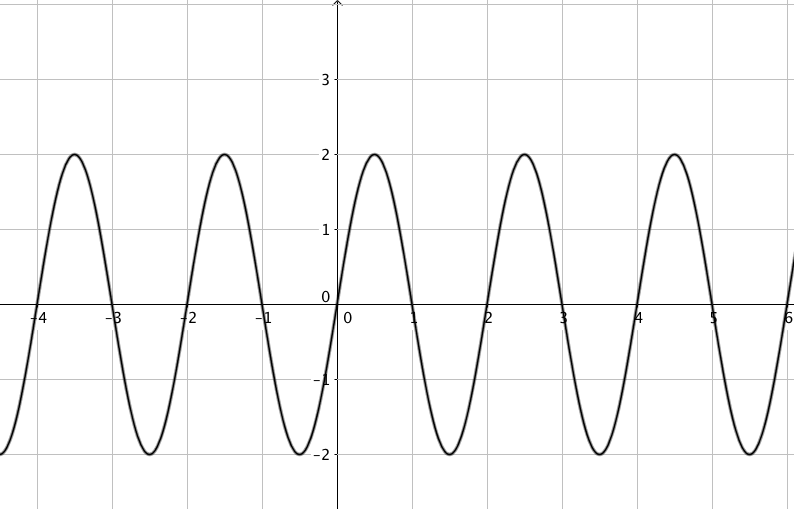
\includegraphics{sineflip}} \\[2in]





\end{enumerate}

\noindent \textbf{Student Learning Outcomes Check}

\begin{enumerate}
\item Can you transform graphs of functions?
\item Do you understand the difference between a shift and a reflection?  Or vertical and horizontal transformations?
\end{enumerate}

\noindent \textbf{If any of your answers were no, please ask about these topics in class.}




\actTitle{1.7 - Piecewise Define Functions and Analysis of Graphs}

\videoLink{Section 1.7}{https://www.youtube.com/playlist?list=PLYHZK3b8UFw0MGYUVN9Z4aYof_QgbFw7f}

\noindent \textbf{Topics:}  basic functions, even and odd functions, graphing piecewise functions, relative minima and maxima\\

\noindent \textbf{Student Learning Outcomes:}
\begin{enumerate}
\item Students will be able to determine whether a function is even, odd, or neither.
\item Students will be able to graph a piecewise function.
\item Students will be able to determine where a function is increasing, decreasing, or constant.
\item  Students will be able to locate relative minimum and relative maximum values of a function on a graph.
\end{enumerate}

\hrule 

\bigskip

\subsection{Even and Odd Functions} ~


\noindent \begin{tabular}{| l |} \hline
We call $f$ an \emph{even} function if the graph of $f$ is symmetric with respect to the $y$ axis.\\ In that case, $f(-x)=f(x)$ for every $x$ in the domain. \\ \hline
\end{tabular}



\noindent \begin{tabular}{| l |} \hline
We call $f$ an \emph{odd} function if the graph of $f$ is symmetric with respect to the origin.\\ In that case, $f(-x)=-f(x)$ for every $x$ in the domain. \\ \hline
\end{tabular}



\begin{enumerate}
\item Determine whether $f$ is even, odd, or neither. 
\begin{enumerate}
\item $f(x)=17x^3-12x^5$\\[1in]
\item $f(x)=x^3-5x^2$\\[1in]
\item $f(x)=|x|$ This is the \emph{absolute value function}. \\[1in]%Sketch its graph below.
\end{enumerate}



\newpage


\subsection{Piecewise-Defined Functions} ~

\hspace{-.4in} \begin{tabular}{| l |} \hline \underline{Piecewise-Defined Functions.}  \\
A \emph{piecewise function} is a function defined by multiple sub-functions with each sub-function applying\\ to a certain interval of the main function's domain.\\
 \hline
\end{tabular}



\item Evaluate the function for the given values of $x$ and then graph the function.
\[
  f(x) =
  \begin{cases}
                                   -x-1 & \text{for $x<1$} \\
                                   -3 & \text{for $1 \leq x <2$} \\
  \sqrt{x-2} & \text{for $x \geq 2$}
  \end{cases}
\]

\begin{enumerate}
\item $f(-3)=$\\[.2in]
\item $f(1)=$ \\[.2in]
\item $f(2)=$ \\[.2in]
\item $f(6)=$ \\[.2in]
\item Graph $f(x)$
\end{enumerate}


      \begin{tikzpicture}[y=0.5cm, x=0.5cm,font=\sffamily]
        \begin{scope} %[shift={(0,8)}]
          %% ticks
          \draw[xstep = 1, ystep=1.0,black,dashed,thick] % very thin,opacity=0.85,
                 (-6.0,-6.0) grid ( 6.0, 6.0);
             %% axis
           \draw[ultra thick,->] (-6.5,0) -- coordinate (x axis mid) (6.5,0)
                node[anchor = north west] {$x$}; 
           \draw[ultra thick,->] (0,-6.5) -- coordinate (y axis mid) (0,6.5) 
                node[anchor = east,shift={(-0.2,-0.2)}]  {$y$};

           %\foreach \y in {-1,1,...,4} {
           %   \draw (1pt, \y) -- (-1pt, \y) node[yshift=-6,xshift=1,anchor=west] {$\y$};
           % }
           %\foreach \x in {-3,-2,-1,1,2,3} {
           %   \draw (\x,1pt) -- (\x,-1pt) node[yshift=-5,xshift=-1,anchor=east] {$\x$};
           % }

          \end{scope}
        \end{tikzpicture}



\newpage



\item Graph the piecewise function.
\[
  f(x) =
  \begin{cases}
                                   x+3 & \text{for $x<-1$} \\
                                   x^2 & \text{for $-1 \leq x <2$} 
  \end{cases}
\]

      \begin{tikzpicture}[y=0.5cm, x=0.5cm,font=\sffamily]
        \begin{scope} %[shift={(0,8)}]
          %% ticks
          \draw[xstep = 1, ystep=1.0,black,dashed,thick] % very thin,opacity=0.85,
                 (-6.0,-6.0) grid ( 6.0, 6.0);
             %% axis
           \draw[ultra thick,->] (-6.5,0) -- coordinate (x axis mid) (6.5,0)
                node[anchor = north west] {$x$}; 
           \draw[ultra thick,->] (0,-6.5) -- coordinate (y axis mid) (0,6.5) 
                node[anchor = east,shift={(-0.2,-0.2)}]  {$y$};

           %\foreach \y in {-1,1,...,4} {
           %   \draw (1pt, \y) -- (-1pt, \y) node[yshift=-6,xshift=1,anchor=west] {$\y$};
           % }
           %\foreach \x in {-3,-2,-1,1,2,3} {
           %   \draw (\x,1pt) -- (\x,-1pt) node[yshift=-5,xshift=-1,anchor=east] {$\x$};
           % }

          \end{scope}
        \end{tikzpicture}

\subsection{Intervals of Increasing, Decreasing, and Constant Behavior}
When looking at functions on a graph, we read from left to right.
And when we talk about function values, we mean values on the $y$-axis.\\[.1in]

In this section, we will determine intervals on the $x$-axis where the
function values on the $y$-axis are increasing, decreasing, or
constant.

\item Determine where the following function is increasing, decreasing, or constant.

      \begin{tikzpicture}[y=0.8cm, x=0.8cm,font=\sffamily]
        \begin{scope} %[shift={(0,8)}]
          %% ticks
          \draw[xstep = 1, ystep=1.0,black,dashed,thick] % very thin,opacity=0.85,
                 (-4.0,-2.0) grid ( 4.0, 5.0);
             %% axis
           \draw[ultra thick,->] (-4.5,0) -- coordinate (x axis mid) (4.5,0)
                node[anchor = north west] {$x$}; 
           \draw[ultra thick,->] (0,-2.5) -- coordinate (y axis mid) (0,5.5) 
                node[anchor = east,shift={(-0.2,-0.2)}]  {$y$};

           \foreach \y in {-2,-1,2,3,4} {
              \draw (1pt, \y) -- (-1pt, \y) node[yshift=-6,xshift=1,anchor=west] {$\y$};
            }
           \foreach \x in {-4,-3,-2,-1,1,2,3,4} {
              \draw (\x,1pt) -- (\x,-1pt) node[yshift=-5,xshift=-1,anchor=east] {$\x$};
            }
          \end{scope}

          \begin{scope}
            \draw[ultra thick,<-] plot [smooth] coordinates
                {(-2.3,5) (-2,4) (-1,1) (0,0) (1,1) };
            \fill[black] (1,1) circle [radius=0.6ex]; 

            \draw[black,ultra thick] (1,3) -- (2,3);
            \fill[black] (1,3) circle [radius=0.6ex]; % Draw an open dot on the 
            \fill[white] (1,3) circle [radius=0.3ex]; 
            \fill[black] (2,3) circle [radius=0.6ex]; % Draw an open dot on the 

            \draw[black,ultra thick,->] (2,2) -- (4,4);
            \fill[black] (2,2) circle [radius=0.6ex]; % Draw an open dot on the 
            \fill[white] (2,2) circle [radius=0.3ex]; 

          \end{scope}
        \end{tikzpicture}

\clearpage

\subsection{Relative Minimum and Relative Maximum Values}
Remember, when talking about function \textbf{values}, we mean
$y$-values.  So in this section we will determine the relative minimum
and maximum $y$-values of a function.

\item For the graph of $y=f(x)$ shown.

        \begin{tikzpicture}[y=0.33cm, x=0.66cm,font=\sffamily]
          \begin{scope} %[shift={(0,8)}]
          %% ticks
          \draw[xstep = 1, ystep=2.0,black,dashed,thick] % very thin,opacity=0.85,
                 (-7.0,-16.0) grid ( 7.0, 4.0);
             %% axis
           \draw[ultra thick,->] (-7.5,0) -- coordinate (x axis mid) (7.5,0)
                node[anchor = north west] {$x$}; 
           \draw[ultra thick,->] (0,-16.5) -- coordinate (y axis mid) (0,4.5) 
                node[anchor = east,shift={(-0.2,-0.2)}]  {$y$};

           \foreach \y in {-16,-14,...,-2,2,4} {
              \draw (1pt, \y) -- (-1pt, \y) node[yshift=-4,xshift=0,anchor=east] {$\y$};
            }
           \foreach \x in {-6,-4,-2,2,4,6} {
              \draw (\x,1pt) -- (\x,-1pt) node[yshift=0,xshift=5,anchor=north] {$\x$};
            }
          \end{scope}

          \begin{scope}
            \draw[ultra thick,<->] plot [smooth] coordinates
            {(-5.3,4) (-3.8,-14.5) (-1.7,-6) (0,-9)
             (1.7,-6) (3.8,-14.5) (5.3,4) };
          \end{scope}
        \end{tikzpicture}

\begin{enumerate}
\item Determine the location and value of any relative maxima.\\[.3in]
\item Determine the location and value of any relative minima.
\end{enumerate}

\vfill
\end{enumerate}

\noindent \textbf{Student Learning Outcomes Check}

\begin{enumerate}
\item Can you determine whether a function is even, odd, or neither?
\item Can you graph a piecewise function?
\item Are you able to determine where a function is increasing, decreasing, or constant?
\item  Can you locate relative minimum and relative maximum values of a function on a graph?

\end{enumerate}

\noindent \textbf{If any of your answers were no, please ask about these topics in class.}



\actTitle{1.8 - Algebra of Functions and Function Composition}

\videoLink{Section 1.8}{https://www.youtube.com/playlist?list=PLYHZK3b8UFw2GleEiLibLzFIsnrHdy43\_}

\noindent \textbf{Topics:}  basic operations on functions, composition of functions, and difference quotient\\

\noindent \textbf{Student Learning Outcomes:}
\begin{enumerate}
\item Students will be able to perform basic operations on functions.
\item Students will be able to compose functions.
\item Students will be able to evaluate a difference quotient.
\end{enumerate}

\hrule 

\bigskip

\subsection{Algebra on Functions}


\begin{enumerate}
\item Find the following values for the functions $f(x) = x + 3$ and $g(x) = x^2$.
\begin{enumerate}
\item $(f+g)(2)$ \vfill 
\item $(f-g)(7)$ \vfill
\item $(fg)(5)$ \\(same as $(f\cdot g )(5)$)\vfill
\item $(f/g)(4)$\vfill
\end{enumerate}




\newpage


\subsection{Function Composition}
The composition of two functions, $f(x)$ and $g(x)$, is given by
	$$(f \circ g)(x)=f[g(x)] \quad \quad \text{or} \quad \quad (g \circ f)(x)=g[f(x)]$$
that is, by "plugging one function into another". One must be careful, however, as the above two quantities are \textbf{\underline{not equal}} in general (it is also important not to confuse this notation with multiplying two functions, hence the use of the "open circle" symbol).

\item Find the following values for the functions $f(x) = x + 3$ and $g(x) = x^2$.
\begin{enumerate}
\item $f(g(4))$\\[1in]
\item $g(f(4))$\\[1in]

\end{enumerate}


\item Use $f(x) = \dfrac{1}{3-x}$ and $g(x)=3x^2-16$ to answer the following.
\begin{enumerate}
\item Determine $f(g(x))$ and the domain of $f(g(x))$. \\[1in]
\item Determine $(g \circ f)(x)$ and the domain of $(g \circ f)(x)$. \\[1in]
%\item Determine $(g \circ g)(x)$. \\ \\ 

\item Determine $g(f(3))$. \\ \\
\end{enumerate}



\newpage

\item \textbf{Decomposition}  Find functions $f$, $g$, such that $f(g(x))=y$ for the function $y = 6 + \sqrt{9-x^2}$. (There is more than one correct answer.) \\[1in]

\item Use the graphs of $f$ and $g$ below to determine the following.
\begin{enumerate}
\item $f (g(2))$  \\[.5in] 
\item $g(f(4))$  \\[.5in] 
\item $f(g(1))$ \\[.5in] 

\end{enumerate}

      \begin{tikzpicture}[y=1.2cm, x=1.2cm,font=\sffamily]
        \begin{scope} %[shift={(0,8)}]
          %% ticks
          \draw[xstep = 1, ystep=1.0,black,dashed,thick] % very thin,opacity=0.85,
                 (-1.0,-1.0) grid ( 5.0, 4.0);
             %% axis
           \draw[ultra thick,->] (-1.5,0) -- coordinate (x axis mid) (5.5,0)
                node[anchor = north west] {$x$}; 
           \draw[ultra thick,->] (0,-1.5) -- coordinate (y axis mid) (0,4.5) 
                node[anchor = east,shift={(-0.2,-0.2)}]  {$y$};

           \foreach \y in {-1,1,2,3,4} {
              \draw (1pt, \y) -- (-1pt, \y) node[yshift=-6,xshift=1,anchor=west] {$\y$};
            }
           \foreach \x in {-1,1,2,3,4,5} {
              \draw (\x,1pt) -- (\x,-1pt) node[yshift=-5,xshift=-1,anchor=east] {$\x$};
            }

            \draw[ultra thick,<->] plot [smooth] coordinates
                {(1,-1) (2,3) (3,1) (4,-1) (5,3) (5.2,4) }
                node[anchor=south east] {$y=f(x)$};

         \end{scope}

        \begin{scope}[shift={(8,0)}]
          %% ticks
          \draw[xstep = 1, ystep=1.0,black,dashed,thick] % very thin,opacity=0.85,
                 (-1.0,-1.0) grid ( 4.0, 4.0);
             %% axis
           \draw[ultra thick,->] (-1.5,0) -- coordinate (x axis mid) (4.5,0)
                node[anchor = north west] {$x$}; 
           \draw[ultra thick,->] (0,-1.5) -- coordinate (y axis mid) (0,4.5) 
                node[anchor = east,shift={(-0.2,-0.2)}]  {$y$};

           \foreach \y in {-1,1,2,3,4} {
              \draw (1pt, \y) -- (-1pt, \y) node[yshift=-6,xshift=1,anchor=west] {$\y$};
            }
           \foreach \x in {-1,1,2,3,4} {
              \draw (\x,1pt) -- (\x,-1pt) node[yshift=-5,xshift=-1,anchor=east] {$\x$};
            }
            
            \draw[ultra thick,<->] plot [smooth] coordinates
                {(-1.2,-1) (-1,0) (0,3) (1,4) (2,3) (3,0) (3.2,-1) }
                node[anchor=north west] {$y=g(x)$};
          \end{scope}

        \end{tikzpicture}


\newpage

\subsection{Diference Quotient}

\textbf{Recall:}The slope of a line through two points $(x_1, y_1)$ and $(x_2, y_2)$ is given by the formula
$$m=\frac{y_2-y_1}{x_2-x_1}=\frac{\Delta y}{\Delta x}=\frac{\text{change in y}}{\text{change in x}}$$


\textbf{Average Rate of Change}\\


 The \textbf{\emph{average rate of change}} of $y=f(x)$ with respect to $x$ over the interval $[x_1,x_2]$ is
 $$\frac{\Delta y}{\Delta x}=\frac{f(x_2)-f(x_1)}{x_2-x_1}=\frac{f(x_1+h)-f(x_1)}{h}, h\neq 0.$$\\ 
 
 This is the \textbf{difference quotient.}  Let's draw a graph.
 \vfill
 
 \item Given $f(x)=3x-5$.
 \begin{enumerate}
 \item Find $f(x+h)$.\\[.5in]
 \item Find the difference quotient, $\frac{f(x+h)-f(x)}{h}$.\\[1.5in]
 \end{enumerate}





\end{enumerate}

\noindent \textbf{Student Learning Outcomes Check}

\begin{enumerate}
\item Can you perform basic algebra operations on functions?
\item Can you compose functions two functions?
\item Are you able to evaluate a difference quotient?


\end{enumerate}

\noindent \textbf{If any of your answers were no, please ask about these topics in class.}



\actTitle{2.1 Part 1 - Quadratic Functions and Applications}


\noindent \textbf{Topics:}  quadratic functions, standard equation for  a quadratic, and vertex of a parabola\\

\noindent \textbf{Student Learning Outcomes:}
\begin{enumerate}
\item Students will be able to recognize quadratic functions graphically and algebraically.
\item Students will be able to write the standard equation for a quadratic function.
\item Students will be able to determine the vertex of a parabola.
\end{enumerate}

\hrule 

\bigskip

\subsection{Standard Form of a Quadratic Function} ~

\noindent \underline{Quadratic Formula.} The roots of the equation $ax^2+bx+c=0$ are \begin{tabular}{| l |} \hline \\ $x = \dfrac{-b \pm \sqrt{b^2-4ac}}{2a}$  \\ \\ \hline
\end{tabular} 


\hspace{-.3in}\begin{tabular}{| l |} \hline 
\noindent \underline{Standard Equation of a Parabola.} The standard equation of a parabola is \\
$ y = a(x-h)^2 + k$. The point $(h,k)$ is the vertex of the parabola.
\\ \hline
\end{tabular} 

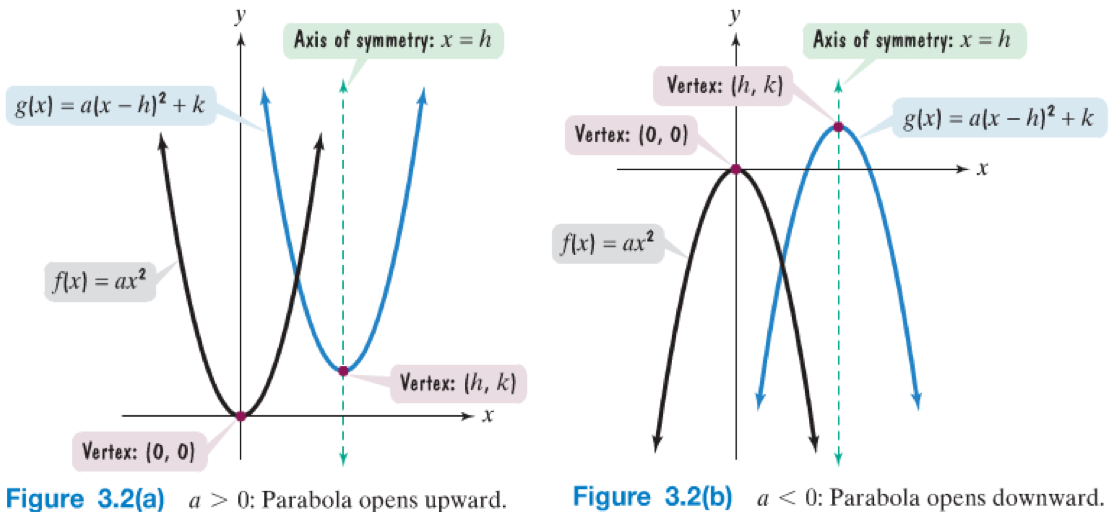
\includegraphics[scale=.7]{graphstandard}



\newpage


\subsection{Graphing a Quadratic Function in Standard Form}

\begin{enumerate}
\item The graph of a quadratic function is given.  Select the function's equation.\\
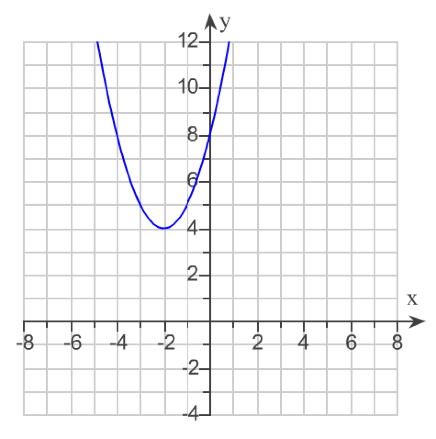
\includegraphics[scale=.7]{quad1a}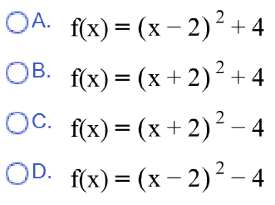
\includegraphics[scale=.7]{quad1b}\\
\item Given $f(x)=-2(x-1)^2+8$
\begin{enumerate}
\item Determine whether the graph of the parabola opens upward or downward.\\[.3in]
\item Identify the vertex.\\[.3in]
\item Determine the $x$-intercept(s).\\[1in]
\item Determine the $y$-intercept.\\[.5in]
\item Sketch the function.\\
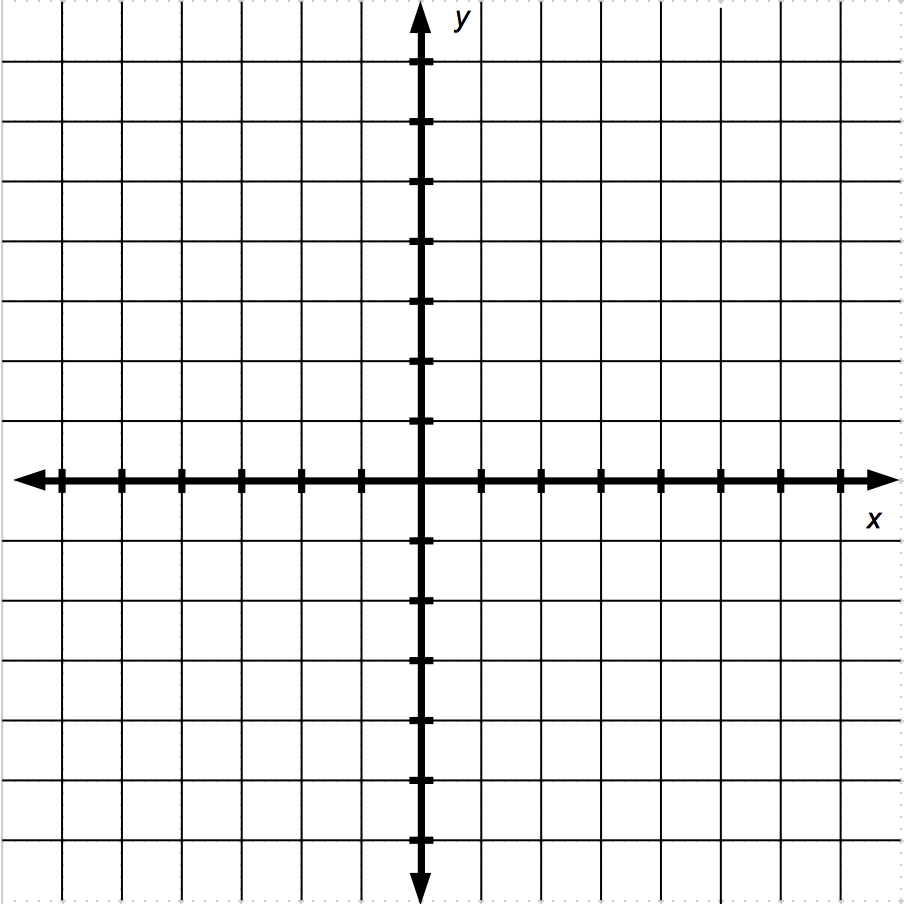
\includegraphics[scale=.5]{bigaxes}\\
\item Determine the axis of symmetry.\\



\end{enumerate}






\newpage



\subsection{Determining the Standard Form of Quadratic Function}

\noindent To determine the standard form of a quadratic function written in the form $y=ax^2+bx+c$, we use a process called \textbf{Completing the Square}.


 
 \item Determine the standard equation of the parabola $y=3x^2+12x+5$.  Then determine the vertex.
 
 
 \vfill
 
  
 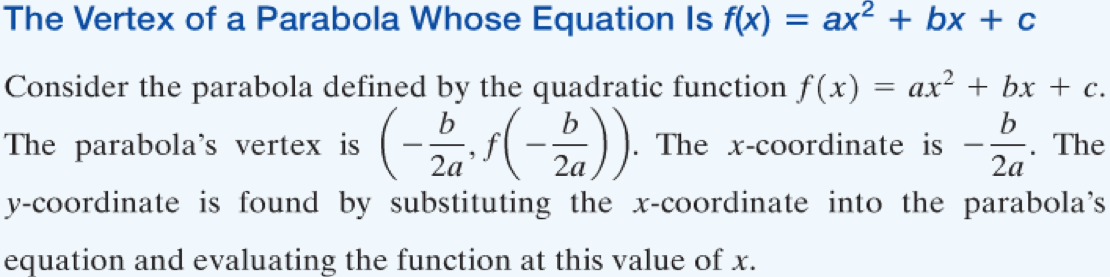
\includegraphics[scale=.75]{parabola}






\end{enumerate}

\noindent \textbf{Student Learning Outcomes Check}

\begin{enumerate}
\item Are you able to recognize quadratic functions graphically and algebraically?
\item Can you write the standard equation for a quadratic function?
\item Are you able to determine the vertex of a parabola?


\end{enumerate}

\noindent \textbf{If any of your answers were no, please ask about these topics in class.}



\actTitle{2.1 Part 2 - Quadratic Functions and Applications}

\noindent \textbf{Topics:}  quadratic functions, applications of quadratic functions\\

\noindent \textbf{Student Learning Outcomes:}
\begin{enumerate}
\item Students will be able to determine a quadratic function given a description.
\item Students will be able to apply a quadratic function to geometry.
\end{enumerate}

\hrule 

\bigskip

\subsection{Solve Applications Involving Quadratic Functions}


\begin{enumerate}
\item A leaping cat follows a parabolic path. The cat jumps a maximum height of 5 feet and covers 6 feet of horizontal ground distance. Find an equation of the form $y = a(x-h)^2+k$ which represents the path of the cat. \vfill

\item An object is projected vertically upward from the top of a building with an initial velocity of 112 ft/sec. Its distance $s(t)$ in feet above the ground after $t$ seconds is given by the equation $s(t)=-16t^2 + 112t + 110.$
\begin{enumerate}
\item Find its maximum distance above the ground.
\item Find the height of the building.
\end{enumerate}

\vfill



\newpage


\subsection{Applying a Quadratic Function to Geometry}


\item A parking area is to be constructed adjacent to a road.  The developer has purchased 340 ft of fencing.  Determine dimensions for the parking lot that would maximize the area.  Then find the maximum area.


\vfill



\end{enumerate}

\noindent \textbf{Student Learning Outcomes Check}

\begin{enumerate}
\item Can you determine a quadratic function given a description?
\item Are you able to apply a quadratic function to geometry?

\end{enumerate}

\noindent \textbf{If any of your answers were no, please ask about these topics in class.}



\actTitle{2.2 - Introduction to Polynomial Functions}

\noindent \textbf{Topics:}  polynomials, leading term test, intermediate value theorem\\

\noindent \textbf{Student Learning Outcomes:}
\begin{enumerate}
\item Students will be able to determine the end behavior of a polynomial function.
\item Students will be able to identify zeros and multiplicities of zeros.
\item Students will be able apply the Intermediate Value Theorem.

\end{enumerate}

\hrule 

\bigskip

\subsection{End Behavior of Polynomial Functions} ~

\begin{boxthm}
{\bf Definition of a Polynomial Function}
Let $n$ be a positive, whole number and $a_n,a_{n-1}, a_{n-2}...,a_1,a_0$ be real numbers, where $a_n\neq 0$.  Then a function defined by $$f(x)=a_nx^n+a_{n-1}x^{n-1}+a_{n-2}x^{n-2}+...+a_1x+a_0$$ is called a \textbf{polynomial function of degree $n$}.

\end{boxthm}


Examples:
$$f(x)=5x^2+8x^4 \quad \quad \quad g(x)=\frac{x^2+3}{x^2} \quad \quad \quad  h(x)=4x^5-3x^4+2x^2 \quad \quad \quad k(x)=4\sqrt{x}-\frac{3}{x} +x^2$$

\vfill
We have already studied several special cases of polynomial functions:

$$f(x)=2 \quad \quad \quad g(x)=3x+1 \quad \quad \quad  h(x)=4x^2+7x-1$$


\vfill

Polynomial functions of degree 2 or higher have graphs that are smooth and continuous.\\[.5in]


\clearpage

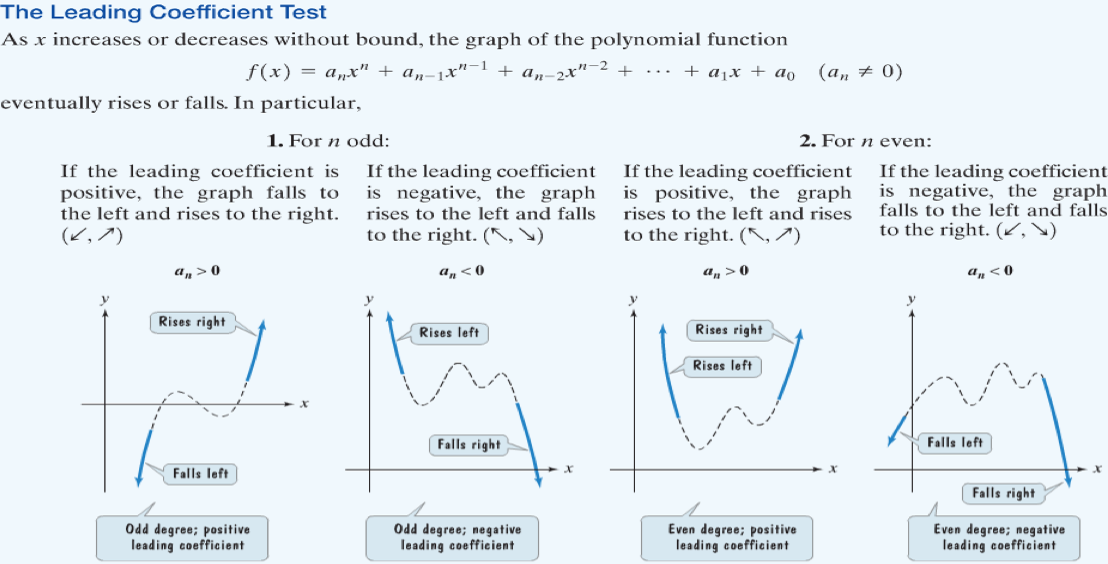
\includegraphics[scale=.95]{poly1}

%\noindent\fcolorbox{gray!10}{blue!10}{%
%\begin{minipage}{\dimexpr1.0\textwidth-2\fboxrule-2\fboxsep\relax}
%some text
%\end{minipage}}%

\subsection{The Leading Coefficient Test}

As $x$ gets very large (positive) or very small (negative), the graph of the
polynomial function
\begin{eqnarray}
  \label{eq:2-2:generalPoly}
  f(x) & = & a_n x^n + a_{n-1} x^{n-1} + a_{n-2} x^{n-2} + \cdots +
             a_1 x + a_0, ~~(a_n \neq 0),
\end{eqnarray}
either rises or falls.

If $n$ is odd:

      \begin{tikzpicture}[y=0.9cm, x=0.9cm,font=\sffamily]
        \begin{scope} %[shift={(0,8)}]
           \draw[ultra thick,->] (-0.5,0) -- coordinate (x axis mid) (4.5,0)
                node[font=\scriptsize,anchor = north west] {$x$}; 
           \draw[ultra thick,->] (0,-2.5) -- coordinate (y axis mid) (0,2.5) 
                node[font=\scriptsize,anchor = west,shift={(0.0,-0.2)}]  {$y$};

           \draw[ultra thick,black,<-]
           (0.5,-2) .. controls +( 0.125,0.5) and +(-0.25, -0.5) .. (0.8,-1)
               node[font=\scriptsize,anchor=west,pos=0] {Falls left};
           \draw[ultra thick,black,->]
           ( 4.4,1) .. controls +( 0.25, 0.5) and +(-0.125,-0.5) .. (4.7,2)
           node[font=\scriptsize,anchor=east,pos=1] {Rises right};

           \draw[ultra thick,black,dashed]
              (0.8,-1)  .. controls +( 0.25, 0.5)  and +(-0.25,-0.4) .. (1.3,0)
              (1.3,0)   .. controls +( 0.25, 0.4)  and +(-0.4,0.0)   .. (2,0.5)
              (2,0.5)   .. controls +( 0.4, 0.0)   and +(-0.25, 0.25) .. (2.7,0)
              (2.7,0)   .. controls +( 0.25,-0.25) and +(-0.4,0.0)   .. (3.4,-.5)
              (3.4,-.5) .. controls +( 0.4, 0.0)  and +(-0.25,-0.5)  .. (4.4,1)
              ;

        \end{scope}

      \end{tikzpicture}



\clearpage

\begin{enumerate}

\item Use the leading term test to determine the function's end behavior.


\begin{enumerate}
\item $f(x)=-7x^5+2x^3+7x+5$
\vfill

\item $f(x)=\frac{1}{4}x(2x-3)^3(x+4)^2$
\vfill

\end{enumerate}

\subsection{Identify Zeros and Multiplicities of Zeros} ~

\begin{boxthm}
{\bf Multiplicities and $x$-Intercepts}
If $f$ is a polynomial function, then the values of $x$ for which $f(x)=0$ are called the \textbf{zeros (roots or solutions)} of $f(x)$.  Each real root of the polynomial equations appears as an $x$-intercept of the graph of the polynomial function.\\
\\
If $r$ is a zero of \textbf{even multiplicity}, then the graph \textbf{touches} the $x$-axis and \textbf{turns around} at $r$.  If $r$ is a zero of \textbf{odd multiplicity}, then the graph \textbf{crosses} the $x$-axis at $r$.  Regardless of whether the multiplicity of a zero is even or odd graphs tend to flatten out near zeros with multiplicity greater than one.
\end{boxthm}




\item Find the zeros for each polynomial function and give the multiplicity for each.  State whether the graph crosses the $x$-axis, or touches the $x$-axis and turns around, at each zero.

\begin{enumerate}
\item $f(x)=4(x+3)(x-7)^2$
\vfill
\item $f(x)=x^3-6x^2+9x$
\vfill
\end{enumerate}


\newpage

\subsection{Apply the Intermediate Value Theorem} ~

\begin{boxthm}
{\bf Intermediate Value Theorem}
Let $f$ be a polynomial function.  For $a<b$, if $f(a)$ and $f(b)$ have opposite signs, then $f$ has at least one zero on the interval $[a,b]$.
\end{boxthm}

\item Use the Intermediate Value Theorem to determine if $f(x)=4x^4-8x^2+2$ has a real zero on the interval $[-1,0]$.
\vfill


\item Sketch a graph of $f(x)=x^3-9x$
\vfill
\vfill
\vfill



\end{enumerate}

\noindent \textbf{Student Learning Outcomes Check}

\begin{enumerate}
\item Are you able to determine the end behavior of a polynomial function?
\item Can you identify zeros and multiplicities of zeros?
\item Are you able apply the Intermediate Value Theorem?
\end{enumerate}

\noindent \textbf{If any of your answers were no, please ask about these topics in class.}


\documentclass[11pt]{article}
\usepackage{amsmath, amssymb, array}
\pagestyle{plain}

\textwidth=6.5in
\hoffset-1in
\textheight=9in
\voffset-1in

\usepackage{enumitem}
\usepackage{pgfplots}
\usepackage{graphicx}
\usepackage{lipsum}
\usepackage{stfloats}
\usepackage{multicol}
\setlength{\columnsep}{1cm}

\newcommand{\boxcolor}{gray!30}
\usepackage{mdframed}
\newenvironment{boxme}{\begin{mdframed}[backgroundcolor=\boxcolor,linewidth=0pt,nobreak=true]}{\end{mdframed}}
\newenvironment{boxthm}{\begin{mdframed}[backgroundcolor=\boxcolor,nobreak=true]}{\end{mdframed}}
\newenvironment{boxdef}{\begin{mdframed}[backgroundcolor=\boxcolor,linewidth=0pt,nobreak=true]}{\end{mdframed}}




\begin{document}


\noindent MATH 1113   \hfill 2.3 - Division of Polynomials and the Remainder and Factor Theorems\\



\noindent \textbf{Topics:}  long division, synthetic division, remainder theorem, factor theorem\\

\noindent \textbf{Student Learning Outcomes:}
\begin{enumerate}
\item Students will be able to divide polynomials using long division.
\item Students will be able to divide polynomials using synthetic division.
\item Students will be able apply the Remainder and Factor Theorems.

\end{enumerate}

\hrule 
\vspace{5mm}

\section{Long Division}

\begin{enumerate}

\item Use long division to divide $(-5+x+4x^2+2x^3+3x^4) \div (x^2+2)$.
\vfill
\vfill

\item Use long division to divide $\displaystyle \frac{2x^2+3x-14}{x-2}$.
\vfill

\newpage




\section{Synthetic Division}
\item Use synthetic division to divide $(-10x^2+2x^3-5) \div (x-4)$.
\vfill


\item Use synthetic division to divide $\displaystyle \frac{x^4+4x^3-2x+18}{x+2}$.
\vfill

\newpage
\section{Remainder and Factor Theorems}
\begin{boxthm}
{\bf Remainder Theorem}
If a polynomial $f(x)$ is divided by $x-c$, then the remainder is $f(c)$.
\end{boxthm}

\textbf{Note:  }The remainder theorem tell us that the value of $f(c)$ is the same as the remainder we get from dividing $f(x)$ by $x-c$.

\item Given $f(x)=x^4+6x^3-12x^2-30x+35$, use the remainder theorem to evaluate $f(2)$.
\vfill

\item Use the remainder theorem to determine if $c=\sqrt{3}$ is a zero of $f(x)=x^3+x^2-3x-3$.
\vfill

\newpage

\begin{boxthm}
{\bf Factor Theorem}
Let $f(x)$ be a polynomial.
\begin{enumerate}
\item If $f(c)=0$, then $(x-c)$ is a factor of $f(x)$.
\item If $(x-c)$ is a factor of $f(x)$, then $f(c)=0$.
\end{enumerate}
\end{boxthm}

\item Use the factor theorem to determine if $x-3$ is a factor of $f(x)=x^4-x^3-11x^2+11x+12$.
\vfill

\item Factor $f(x)=3x^3+25x^2+42x-40$, given that -5 is a zero of $f(x)$.  Then solve the equation $3x^3+25x^2+42x-40=0$.
\vfill
\vfill



\end{enumerate}

\noindent \textbf{Student Learning Outcomes Check}

\begin{enumerate}
\item Can you divide polynomials using long division?
\item Can you divide polynomials using synthetic division?
\item Are you able apply the Remainder and Factor Theorems?

\end{enumerate}

\noindent \textbf{If any of your answers were no, please ask about these topics in class.}













\end{document}

 
\chapter{Exponential and Logarithmic Functions}

\actTitle{3.1 - Inverse Functions}

\videoLink{Section 3.1}{https://www.youtube.com/playlist?list=PLYHZK3b8UFw2aq4QBoSuTAkPcWN5e-afh}

\noindent \textbf{Topics:}  one-to-one functions, inverse functions, domain and range of inverse functions\\

\noindent \textbf{Student Learning Outcomes:}
\begin{enumerate}
\item Students will be able to determine if a function is one-to-one algebraically and graphically.
\item Students will be able to determine the inverse of a function.
\item Students will be able to determine the domain and range of an inverse function.
\end{enumerate}

\hrule 

\bigskip

\subsection{Identify One-to-One Functions} ~


\noindent \begin{tabular}{ | l  |} \hline
\noindent \underline{Horizontal Line Test.} A function is one-to-one if every horizontal line intersects \\ the graph of $f$ at most once. Otherwise the function is not one-to-one. \\  \hline
\end{tabular} 

\begin{enumerate}
\item Determine whether the graph is the graph of a one-to-one function.

      \begin{tikzpicture}[y=0.8cm, x=0.8cm,font=\sffamily]
        \begin{scope} %[shift={(0,8)}]
           \draw[ultra thick,->] (-1.5,0) -- coordinate (x axis mid) (5.5,0)
                node[anchor = north west] {$x$}; 
           \draw[ultra thick,->] (0,-1.5) -- coordinate (y axis mid) (0,4.5) 
                node[anchor = east,shift={(-0.2,-0.2)}]  {$y$};

           \foreach \y in {-1,1,2,3,4} {
              \draw (1pt, \y) -- (-1pt, \y) node[yshift=-6,xshift=-1,anchor=east] {$\y$};
            }
           \foreach \x in {-1,1,2,3,4,5} {
              \draw (\x,1pt) -- (\x,-1pt) node[yshift=-5,xshift=-1,anchor=east] {$\x$};
            }

            \draw[ultra thick,black]
              (1,4)  .. controls +( 0.8, -0.1)  and +(-0.25,0.4) .. (4,2);

            \fill[black] (1,4) circle [radius=0.4ex];
            \fill[black] (4,2) circle [radius=0.4ex]; 
         \end{scope}

        \begin{scope}[shift={(9,0)}]
           \draw[ultra thick,->] (-1.5,0) -- coordinate (x axis mid) (5.5,0)
                node[anchor = north west] {$x$}; 
           \draw[ultra thick,->] (0,-1.5) -- coordinate (y axis mid) (0,4.5) 
                node[anchor = east,shift={(-0.2,-0.2)}]  {$y$};

           \foreach \y in {-1,1,2,3,4} {
              \draw (1pt, \y) -- (-1pt, \y) node[yshift=-6,xshift=-1,anchor=east] {$\y$};
            }
           \foreach \x in {-1,1,2,3,4,5} {
              \draw (\x,1pt) -- (\x,-1pt) node[yshift=-5,xshift=-1,anchor=east] {$\x$};
            }


            \draw[ultra thick,black,dashed]
              (0.0,2)  .. controls +( 0.25,  0.5)  and +(-0.25,0.0)  .. (0.5,3.5)
              (0.5,3.5) .. controls +( 0.25, 0.0)  and +(-0.4,0.0) .. (1.5,0.5)
              (1.5,0.5) .. controls +( 0.4,  0.0)  and +(-0.2,-0.5)   .. (2,2)
              ;

            \fill[black] (0,2) circle [radius=0.4ex];
            \fill[black] (2,2) circle [radius=0.4ex]; 
         \end{scope}
        \end{tikzpicture}


\item Determine whether the following functions are one-to-one.
\begin{enumerate}
\item $f=\{(1,4), (2,3), (-2,3)\}$\\[.5in]

\item $f(x) = \sqrt{5x}$
\vfill
\item $f(x) = x^2$
\end{enumerate}
\vfill


\newpage


\subsection{Determine Whether Two Functions are Inverses} ~


\noindent \begin{tabular}{ | p{0.8\textwidth} |} \hline \noindent
\underline{Theorem on Inverse Functions.} Let $f$ be a one-to-one
function with domain $D$ and range $R$. If $g$ is a function with
domain $R$ and range $D$, then $g$ is the inverse function of $f$
precisely when both of the following conditions hold:

$ \star$ \quad $g(f(x))=x$ for every $x$ in $D$, and \\
$ \star$ \quad $f(g(y))=y$ for every $y$ in $R$.\\ \hline
\end{tabular} 

\noindent \textbf{Notation:} "f inverse" is typically written as
$f^{-1}$. It is important to note that $f^{-1}$ does NOT mean the same
thing as $\dfrac{1}{f}$.

\item Let $f(x) = x^2+4, \quad x \geq 0$, and let $g(x) = \sqrt{x-4}, \quad x \geq 4 $
\begin{enumerate}
\item Use the theorem on inverse functions to determine whether $f$
      and $g$ are inverses.

\vfill

\item Sketch the graphs of $f$ and $g$ on the same coordinate axes. \samepage \\
      \begin{tikzpicture}[y=0.6cm, x=0.6cm,font=\sffamily]
        \begin{scope} %[shift={(0,8)}]
          %% ticks
          \draw[xstep = 1, ystep=1.0,black,dashed,thick] % very thin,opacity=0.85,
                 (-6.0,-6.0) grid ( 6.0, 6.0);
             %% axis
           \draw[ultra thick,->] (-6.5,0) -- coordinate (x axis mid) (6.5,0)
                node[anchor = north west] {$x$}; 
           \draw[ultra thick,->] (0,-6.5) -- coordinate (y axis mid) (0,6.5) 
                node[anchor = east,shift={(-0.2,-0.2)}]  {$y$};

           %\foreach \y in {-1,1,...,4} {
           %   \draw (1pt, \y) -- (-1pt, \y) node[yshift=-6,xshift=1,anchor=west] {$\y$};
           % }
           %\foreach \x in {-3,-2,-1,1,2,3} {
           %   \draw (\x,1pt) -- (\x,-1pt) node[yshift=-5,xshift=-1,anchor=east] {$\x$};
           % }

          \end{scope}
        \end{tikzpicture}
\end{enumerate}

\clearpage

\subsection{Find the Inverse of a Function} ~

\noindent \begin{tabular}{ | l  |} \hline
\noindent \underline{Guidelines for Finding Inverse Functions.} \\
Assuming that $f$ is a one-to-one function, and that the algebra is do-able, you can find $f^{-1}$ \\ using the following procedure: \\
1. Solve the equation $y=f(x)$ for $x$ in terms of $y$. You now have $x = f^{-1}(y)$. \\
2. Replace $x$ with $y$ and solve for $y$. This is your inverse function, replace $y$ with $f^{-1}(x)$. \\ 
3. Check your work (if time permits): check that $f^{-1}(f(x))=x$ whenever $x$ is in the domain\\ of $f$, and $f(f^{-1}(x))=x$ whenever $x$ is in the domain of $f^{-1}$. \\ \hline
\end{tabular} 


 
 \item Find the inverse function of $f(x) = 4 + 3x$. \\[1.2in]
 
 
 \vfill
 
  
\item Use the table for the one-to-one function $f(x)$ to compute each expression.\\[.2in]
\begin{tabular}{| c |  c | c | c | c | c | }
\hline x & 2 & 3&7 &6 & 15\\ \hline
f(x) &-1 &5 &4 &2 & 3\\ \hline
\end{tabular} 
\\
\begin{enumerate}
\item $f^{-1} (5)$ \\ \\
\item $f^{-1} (-1)$ \\ \\
\item $f^{-1} (2)$ \\ \\

\end{enumerate}




\end{enumerate}

\noindent \textbf{Student Learning Outcomes Check}

\begin{enumerate}
\item Can you determine if a function is one-to-one algebraically and graphically?
\item Are you able to determine the inverse of a function?
\item Can you determine the domain and range of an inverse function?

\end{enumerate}

\noindent \textbf{If any of your answers were no, please ask about these topics in class.}




\actTitle{3.2 - Exponential Functions}



\noindent \textbf{Topics:}  exponential functions, compound interest, the number $e$, exponential functions with base $e$, growth and decay\\

\noindent \textbf{Student Learning Outcomes:}
\begin{enumerate}
\item Students will be able to recognize an exponential function graphically and algebraically.
\item Students will be able to evaluate the exponential function base $e$.
\item Students will be able to use exponential functions in compound interest and growth/decay problems.
\end{enumerate}

\hrule 

\bigskip

\subsection{Exponential Functions} ~

\noindent\underline{Exponential functions $y=a^x$} (always assume $a>0$) \\[.2in]

\begin{center}
\begin{tabular}{l | l}
exponential growth: $a>1$      & exponential decay: $0<a<1$ \\
Ex. $f(x)=3^x$ & Ex. $g(x)=\left(\dfrac{1}{2}\right)^x$ \\
\scalebox{0.4}{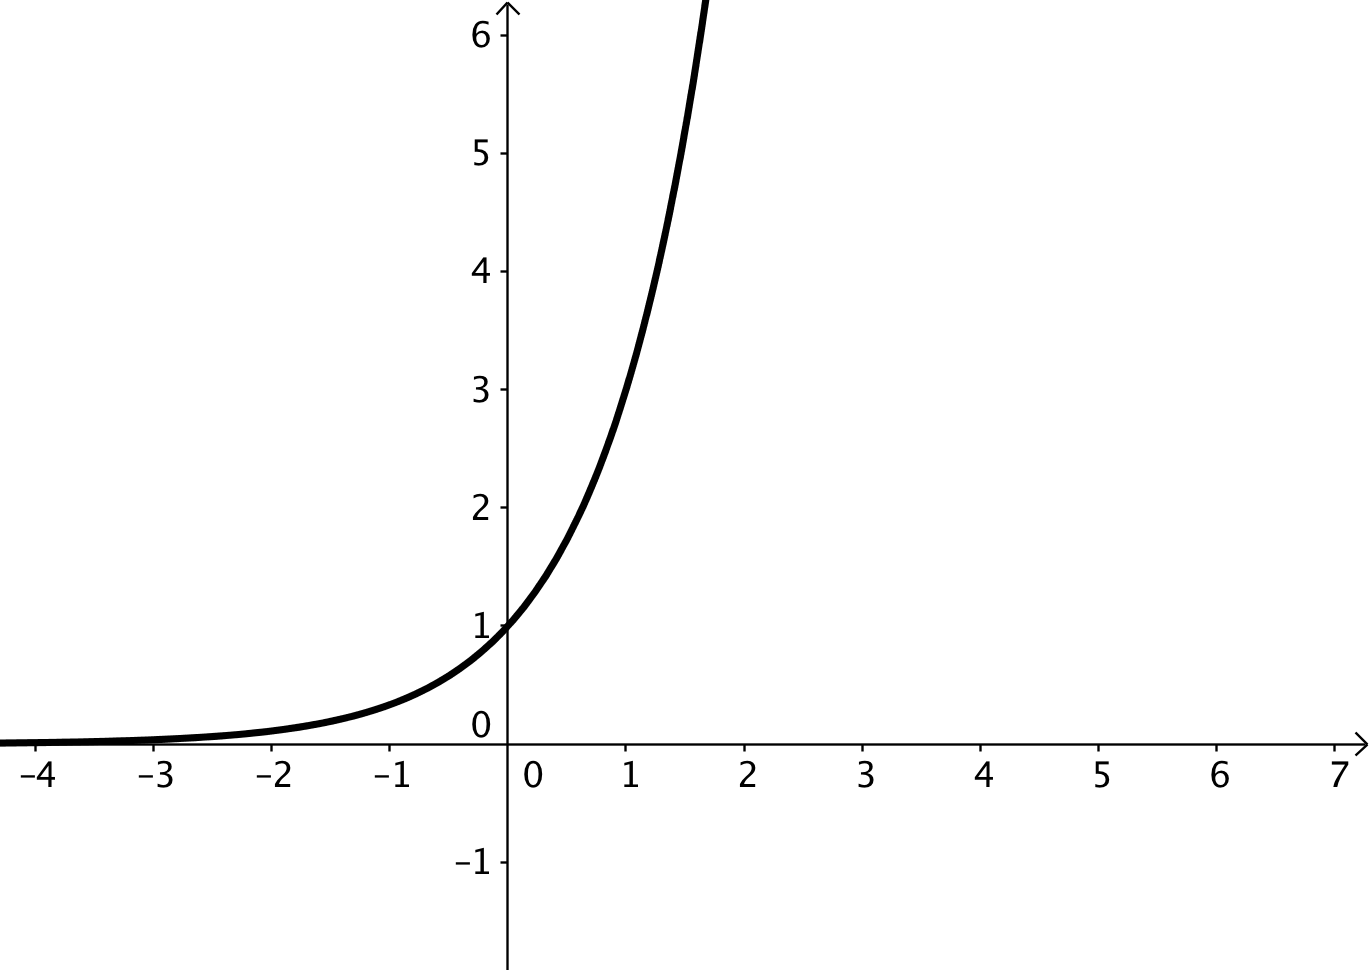
\includegraphics{exp1}} &   \scalebox{0.4}{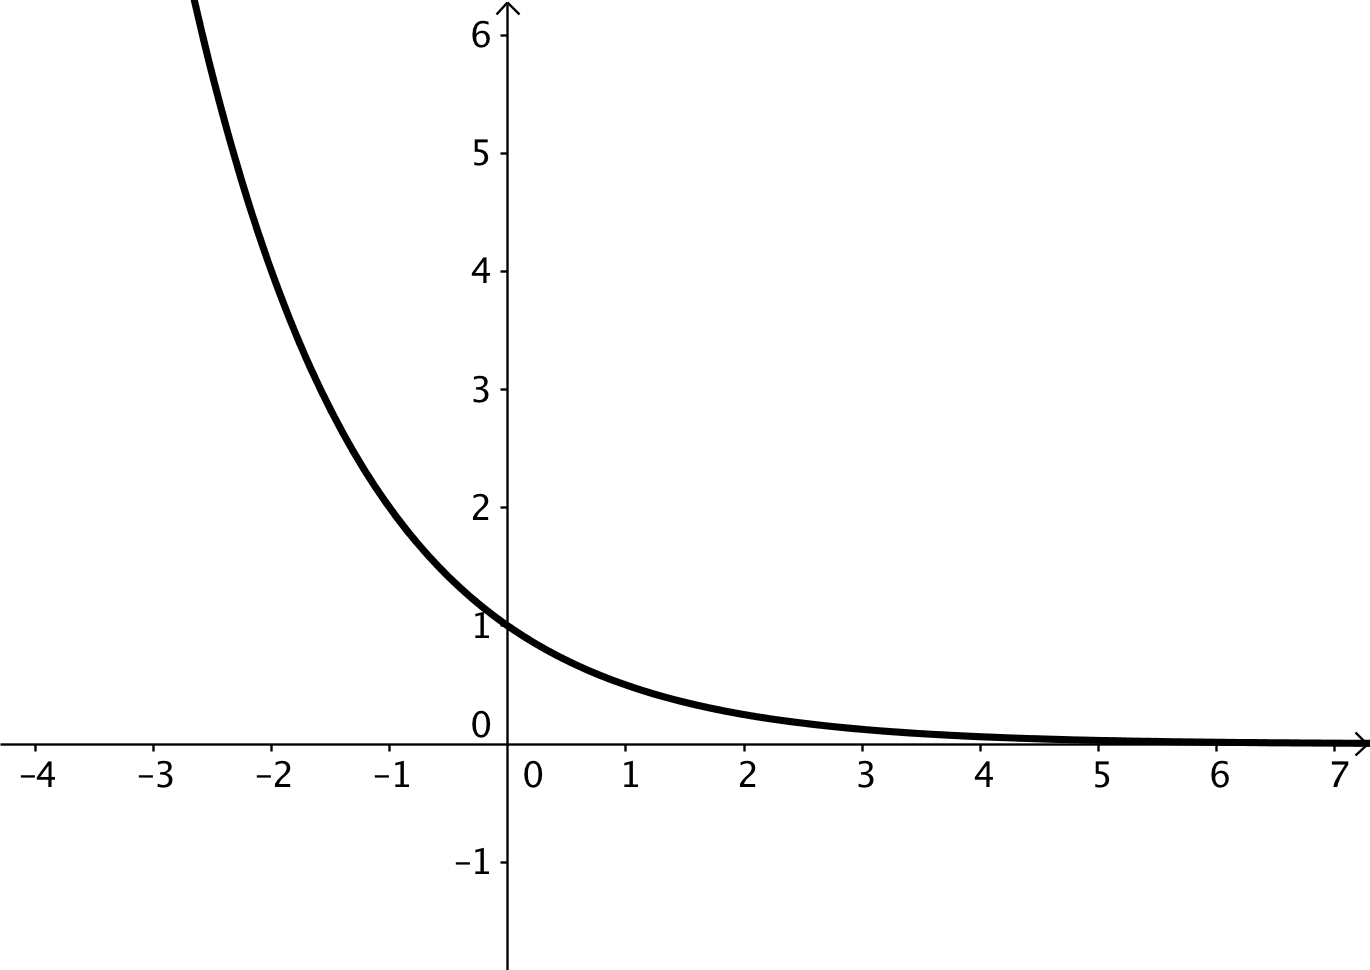
\includegraphics{exp2}} \\
always increasing & always decreasing \\
one-to-one & one-to-one \\
has an asymptote of $y=0$  & has an asymptote of $y=0$ \\
$y$-intercept is $(0,1)$, no $x$-intercept & $y$-intercept is $(0,1)$,  no $x$-intercept  \\
\end{tabular} 
\end{center}

\scalebox{0.9}{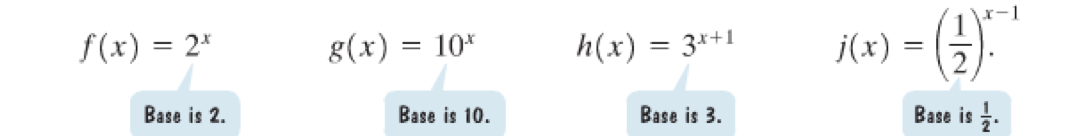
\includegraphics{expex}} 



\begin{enumerate}

\item Is $f(x)=1^x$ an exponential function?\\[.5in]



\item Is $f(x)=(-4)^x$ an exponential function?\\


\newpage
\item Graph $f(x)=3^{x-2}+4.$\\
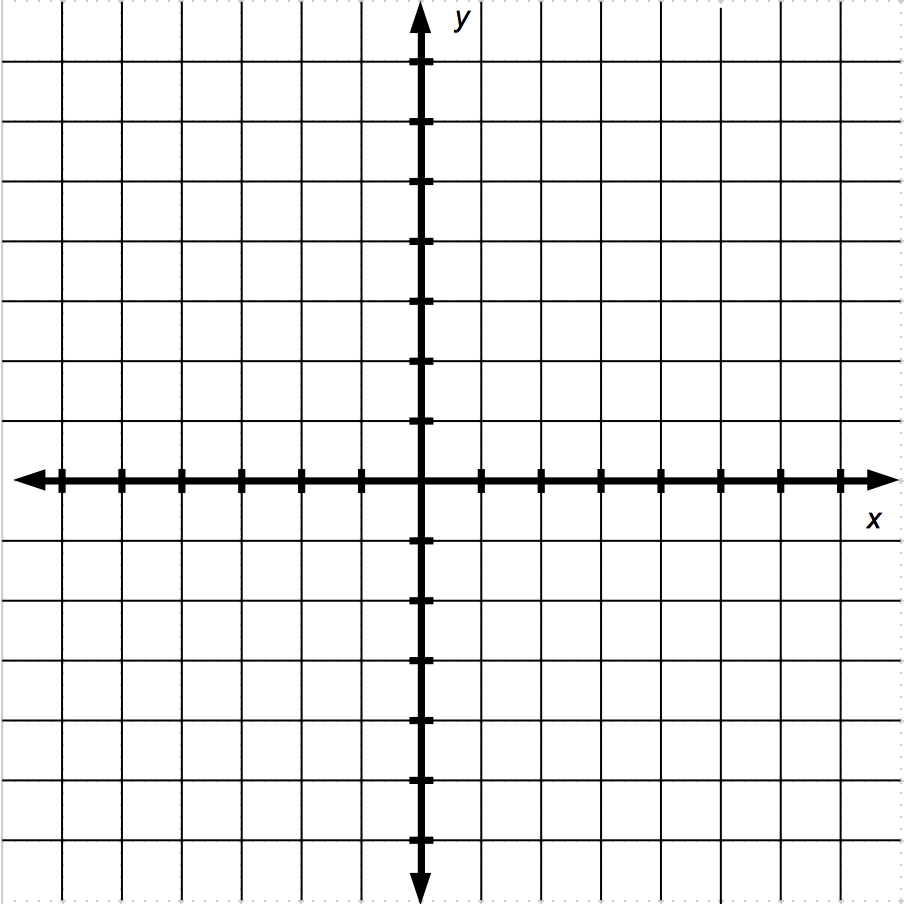
\includegraphics[scale=.5]{bigaxes}

\item Determine the domain and range of $y=5^{x-3}+4$.  \\[1in]





\subsection{Exponential Function Base $e$} 
Just like the number $\pi \approx 3.14159$ is important to the study
of circles and angle measures, the number $e \approx 2.71828$ is
important to problems involving exponential exponential functions (and
their inverses).

Where does the number $e$ come from? Consider the expression $$\Bigg(1+\frac{1}{n}\Bigg)^n$$
If you plug in larger and larger values for $n$, this expression gets closer and closer to $e$.  Try it out!\\
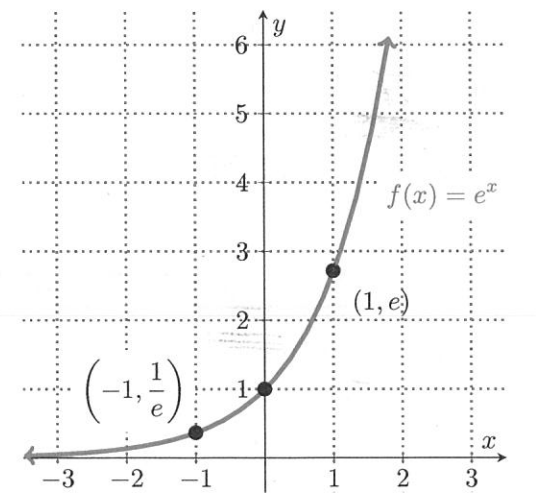
\includegraphics[scale=.8]{e}





\subsection{Compound Interest} ~

\hspace{-.3in} \begin{tabular}{ | l  |} \hline 
\noindent \underline{Compound Interest Formula (Annually, Monthly, Quarterly, Daily, Etc.)}  
$A= P \left( 1+ \dfrac{r}{n} \right)^{nt}$ \\ 
In this formula, $P$ is the principal, $r$ is the annual interest rate in decimal form, $n$ is\\ the number of interest periods per year, $t$ is the number of years $P$ is invested, and $A$ is the\\ amount after $t$ years. \\ \hline
\end{tabular} 

\item Suppose \$ 2000 is invested at a rate of $3 \%$ compounded monthly. Find the \emph{principal after 18 months}. (Round your answer to the nearest cent.) \vfill


 \hspace{-.3in} \begin{tabular}{| l |} \hline
\underline{Continuously compounded interest formula} $A = Pe^{rt}$ \\
In this formula, $P$ is the principal, $r$ is the annual interest rate in decimal form, 
$t$ is the\\ number of years $P$ is invested, and
$A$ is the amount after $t$ years.   \\ \hline
\end{tabular}


\item If \$1500 is deposited in a savings account that pays interest at a rate of .1\% compounded continuously, find the balance after 7 years. \\[1in]


\newpage

\subsection{Exponential Functions in Applications} 
Increasing and decreasing exponential functions can be used in a
variety of real world applications.  For example:
\begin{itemize}
\item Population growth can often be modeled by an exponential function.
\item The growth of an investment under compound interest increases exponentially.
\item The mass of a radioactive substance decreases exponentially with time.
\end{itemize}

\noindent A substance that undergoes radioactive decay is said to be radioactive.  The \textbf{half-life} of a radioactive substance is the amount of time it takes for one-half of the original amount of the substance to change into something else.

\item The half-life of radium 226 is 1620 years.  In a sample originally having 1 gram of radium 226, the amount $A(t)$ in grams of radium 226 present after $t$ years is given by $\displaystyle A(t)=(\frac{1}{2})^{t/1620}$ where $t$ is the time in years after the start of the experiment.  How much radium will be present after 3240 years? 
\vfill


\end{enumerate}

\noindent \textbf{Student Learning Outcomes Check}

\begin{enumerate}
\item Can you recognize an exponential function graphically and algebraically?
\item Can you evaluate the exponential function base $e$?
\item Are you able to use exponential functions in compound interest and growth/decay problems?

\end{enumerate}

\noindent \textbf{If any of your answers were no, please ask about these topics in class.}


\actTitle{3.3 - Logarithmic Functions}

\videoLink{Section 3.3}{https://www.youtube.com/playlist?list=PLYHZK3b8UFw0UKAko9PhlIZXI78LYusTN}

\noindent \textbf{Topics:}  exponential functions, compound interest, the number $e$, exponential functions with base $e$, growth and decay\\

\noindent \textbf{Student Learning Outcomes:}
\begin{enumerate}
\item Students will be able to recognize a logarithic function graphically and algebraically.
\item Students will be able to evaluate the logarithmic expressions.
\item Students will be able to apply basic logarithmic properties.
\end{enumerate}

\hrule 

\bigskip

\subsection{Logarithmic Functions} ~

\noindent\begin{tabular}{ | l  |} \hline
\noindent  Let $a$ be a positive real number different from 1. The \emph{logarithm of $x$ with base $a$} is defined by   \\
\hspace{1.5in} $y = \log_a(x)$    if and only if   $a^y=x$. \\  \hline
\end{tabular} \\

\noindent Above, the left-hand equation is said to be in
\emph{logarithmic form}, while the right-hand equation is said to be
in \emph{exponential form}. The equations are \emph{equivalent}: they
have the same solutions.

\noindent
\begin{tabular}{m{0.4\textwidth}@{\hspace{2em}}m{0.5\textwidth}}
  \begin{tikzpicture}[y=0.7cm, x=0.7cm,font=\sffamily]
    \node[anchor=west] at (0,0) {$\log_a(x)=y$ is equivalent to $a^y=x$.};
    \draw[thick,<->] (1.1,-0.3) -- (1.1,-1) 
       node[anchor=north west,yshift=-1,pos=1] {$a$ is the base.}
       -- (7.5,-1) -- (7.5,-0.3);
    \draw[thick,<->] (3,0.5) -- (3,1.2)
       node[anchor=south west,yshift=1,pos=1] {$y$ is the exponent.}
       -- (7.7,1.2) -- (7.7,0.5);
     \end{tikzpicture}
  &
  \begin{tikzpicture}[y=0.7cm, x=0.7cm,font=\sffamily]
    \begin{scope}
      %% ticks
      \draw[step = 1.0, gray,dashed] (-1,-2) grid (8,4);
      %% axis
      \draw[thick,->] (-1.5,0) -- coordinate (x axis mid) (8.5,0)
          node[anchor = north west] {$x$};
      \draw[thick,->] (0,-2.5) -- coordinate (y axis mid) (0,4.5) node[anchor=west] {$y$};

      \foreach \y in {-1,1,2,3,4} {
        \draw (1pt, \y) -- (-1pt, \y)
            node[font=\scriptsize,yshift=-6,xshift=-1,anchor=east] {$\y$};
      }
      \foreach \x in {-1,1,2,3,4,5,6,7,8} {
        \draw (\x,1pt) -- (\x,-1pt) node[font=\scriptsize,yshift=-5,xshift=3,anchor=east] {$\x$};
      }

      \node[anchor=west,align=left] at (-0.5,5.5) {Example: $f(x)=\log_2(x)$};
      
      \begin{scope}
        %% \clip(-4,-1) rectangle (8,5);
        \draw[scale=1.0,domain=0.17:8,smooth,variable=\x,very thick,black,samples=100,<->]
            plot ({\x},{ln(\x)/ln(2)}) node[anchor=south west] {$\log_2(x)$};
      \end{scope}
     \end{scope}

  \end{tikzpicture}
\end{tabular}

\begin{enumerate}
\item Write in exponential form.  \\
model: $\log_a(x)=y$ \hspace{1in} $\log_2 (16) = 4$ \hspace{1in} $\log_p (13) = y$\\[1in]

\item Write in logarithmic form. \\
model: $a^y = x$  \hspace{1in} $4^{-3} = \dfrac{1}{64}$ \hspace{1in} $\pi^t = 9.4$ \\[.5in]


\item The expression $\log x$, called the \emph{common logarithm}, is shorthand for $\log_{10}(x)$. Write in logarithmic form: $10^{2x+3} = 7$. \\[.5in]


\item The expression $\log x$, called the \emph{common logarithm}, is shorthand for $\log_{10}(x)$. Write in logarithmic form: $10^{2x+3} = 7$. \\[.5in]

\item Find the domain of the function $f(x) = \ln (9-6x)$. \\[.8in]



\subsection{Evaluating Logarithmic Expressions}
  
\item Find the number, if possible. Rewrite in exponential form,
  either to solve, or to check.
  \begin{eqnarray*}
    \begin{array}{c@{\hspace{6em}}c@{\hspace{6em}}c@{\hspace{6em}}c}
      \log_2 \left(  \dfrac{1}{8} \right)    &
      \log_3 (27) &
      \log_4(0) &
      \log_b\left(\dfrac{1}{b^3}\right)
    \end{array}
  \end{eqnarray*}

   \noindent\colorbox{blue!10}{%
   \parbox{\dimexpr\linewidth}%
   {%
     \textbf{Basic Logarithmic Properties Involving One}
     \begin{enumerate}
     \item $\log_b(b)=1$ because when we raise $b$ to the power 1 the result is $b$ ($b^1=b$).
     \item $\log_b(1)=0$ because when we raise $b$ to the power 0 the result is $1$ ($b^0=1$).
     \end{enumerate}

     \textbf{Inverse Properties of Logarithms}
     For $b>0$ and $b\neq 1$:
     \begin{enumerate}
     \item $\log_b\left(b^x\right) = x$ 
     \item $b^{\log_b(x)}=x$ 
     \end{enumerate}
   }
 }


\item Evaluate the common and natural logarithms.
    \begin{eqnarray*}
    \begin{array}{c@{\hspace{6em}}c@{\hspace{6em}}c@{\hspace{6em}}c}
      \log (100,000) &
      \log (0.001) &
      \ln (e^4) &
      \ln \left(\dfrac{1}{e}\right)
    \end{array}
  \end{eqnarray*}

\subsection{Graphing Logarithmic Functions} ~

\noindent
      \begin{tikzpicture}[y=1.05cm, x=1.05cm,font=\sffamily]
        \begin{scope} %[shift={(0,8)}]
           \draw[thick,->] (-3.5,0) -- coordinate (x axis mid) (3.5,0)
                node[anchor = north west] {$x$}; 
           \draw[thick,->] (0,-3.5) -- coordinate (y axis mid) (0,3.5) 
                node[anchor = east,shift={(-0.2,-0.2)}]  {$y$};

            \draw[ultra thick,black]
                (-3.5,0.2)  .. controls +( 2.0, 0.10)  and +(-0.5,-0.25) .. (0,1)
                node[anchor=south east,pos=0.5] {$f(x)=b^x$}
                ( 0.0,1.0)  .. controls +( 0.5, 0.25)  and +(-0.25,-1) .. (2,3.5)
                ;
            \draw[ultra thick,black]
               (0.2,-3.5)  .. controls +( 0.1,2.0)  and +(-0.25,-0.5) .. (1,0)
               node[anchor=north west,pos=0.5] {$f^{-1}(x)=\log_b(x)$}
               ( 1.0,0.0)  .. controls +( 0.25,0.5) and +(-1,-.25) .. (3.5,2);
                
            \draw[thick,dotted] (-3.5,-3.5) -- (3.5,3.5) node[anchor=south west] {$y=x$};

            \fill[black] (0,1) circle [radius=0.6ex] node[anchor=south east] {$(0,1)$};
            \fill[black] (1,0) circle [radius=0.6ex] node[anchor=north west] {$(1,0)$};
            \node[anchor=north] at (0,-3.5) {$b>1$};
            \node[anchor=north,font=\scriptsize,align=left] at (-2,0) {Horizontal asymptote: \\$y=0$};
            \node[anchor=east,font=\scriptsize,align=right] at (0,-3) {Vertical asymptote: \\$x=0$};
          \end{scope}

          \begin{scope}[shift={(8,0)}]
           \draw[thick,->] (-3.5,0) -- coordinate (x axis mid) (3.5,0)
                node[anchor = north west] {$x$}; 
           \draw[thick,->] (0,-3.5) -- coordinate (y axis mid) (0,3.5) 
                node[anchor = east,shift={(-0.2,-0.2)}]  {$y$};

            \draw[ultra thick,black]
            (-2,3.5)  .. controls +( 0.25,-1.0)  and +(-0.5,0.5) .. (0,1)
            node[anchor=east,xshift=-4,pos=0.5] {$f(x)=b^x$}
                ( 0.0,1.0)  .. controls +( 0.5, -0.5)  and +(-2.0,0.1) .. (3.5,0.2)
                ;
            \draw[ultra thick,black]
               (0.2,3.5)  .. controls +(0.1,-1.0)  and +(-0.5,0.5) .. (1,0)
               ( 1.0,0.0)  .. controls +( 0.5,-0.5) and +(-1.5,0.5) .. (3.5,-2)
               node[anchor=east,xshift=-5,pos=1.0] {$f^{-1}(x)=\log_b(x)$}
               ;
            \draw[thick,dotted] (-3.5,-3.5) -- (3.5,3.5) node[anchor=south west] {$y=x$};

            \fill[black] (0,1) circle [radius=0.6ex] node[anchor=north east] {$(0,1)$};
            \fill[black] (1,0) circle [radius=0.6ex] node[anchor=north west,xshift=8] {$(1,0)$};
            \node[anchor=north] at (0,-3.5) {$0<b<1$};
            \node[anchor=north,font=\scriptsize,align=right] at (2.3,1) {Horizontal asymptote: \\$y=0$};
            \node[anchor=west,font=\scriptsize,align=left] at (0.2,3.5) {Vertical asymptote: \\$x=0$};

           \end{scope}
        \end{tikzpicture}


\item Graph $\log_2 x$ and $\log_{1/4} x$\\
      \noindent
      \begin{tikzpicture}[y=0.5cm, x=0.5cm,font=\sffamily]
        \begin{scope} %[shift={(0,8)}]
          %% ticks
          \draw[xstep = 1, ystep=1.0,black,dashed,thick] % very thin,opacity=0.85,
                 (-6.0,-6.0) grid ( 6.0, 6.0);
             %% axis
           \draw[ultra thick,->] (-6.5,0) -- coordinate (x axis mid) (6.5,0)
                node[anchor = north west] {$x$}; 
           \draw[ultra thick,->] (0,-6.5) -- coordinate (y axis mid) (0,6.5) 
                node[anchor = east,shift={(-0.2,-0.2)}]  {$y$};

           %\foreach \y in {-1,1,...,4} {
           %   \draw (1pt, \y) -- (-1pt, \y) node[yshift=-6,xshift=1,anchor=west] {$\y$};
           % }
           %\foreach \x in {-3,-2,-1,1,2,3} {
           %   \draw (\x,1pt) -- (\x,-1pt) node[yshift=-5,xshift=-1,anchor=east] {$\x$};
           % }

          \end{scope}

        \begin{scope} [shift={(15,0)}]
          %% ticks
          \draw[xstep = 1, ystep=1.0,black,dashed,thick] % very thin,opacity=0.85,
                 (-6.0,-6.0) grid ( 6.0, 6.0);
             %% axis
           \draw[ultra thick,->] (-6.5,0) -- coordinate (x axis mid) (6.5,0)
                node[anchor = north west] {$x$}; 
           \draw[ultra thick,->] (0,-6.5) -- coordinate (y axis mid) (0,6.5) 
                node[anchor = east,shift={(-0.2,-0.2)}]  {$y$};

           %\foreach \y in {-1,1,...,4} {
           %   \draw (1pt, \y) -- (-1pt, \y) node[yshift=-6,xshift=1,anchor=west] {$\y$};
           % }
           %\foreach \x in {-3,-2,-1,1,2,3} {
           %   \draw (\x,1pt) -- (\x,-1pt) node[yshift=-5,xshift=-1,anchor=east] {$\x$};
           % }

          \end{scope}

        \end{tikzpicture}


\end{enumerate}

\noindent \textbf{Student Learning Outcomes Check}

\begin{enumerate}
\item Can you recognize a logarithic function graphically and algebraically?
\item Can you evaluate the logarithmic expressions?
\item Are you able to apply basic logarithmic properties?

\end{enumerate}

\noindent \textbf{If any of your answers were no, please ask about these topics in class.}



\actTitle{3.4 - Properties of Logarithms}

\videoLink{Section 3.4}{https://www.youtube.com/playlist?list=PLYHZK3b8UFw3229NnJqFoe05V02x1QMb8}

\noindent \textbf{Topics:}  properties of logarithms, change of base\\

\noindent \textbf{Student Learning Outcomes:}
\begin{enumerate}
\item Students will be able to apply the product, quotient, and power properties of logarithms.
\item Students will be able to write a logarithm in expanded form.
\item Students will be able to write a logarithm as a single logarithm.
\item Students will be able to apply the change of base formula.
\end{enumerate}

\hrule 

\bigskip

\subsection{Properties of Logarithms} ~


\noindent \textbf{Product Property of Logarithms:} Let $b, x,$ and $y$ be positive real numbers where $b \neq 1.$  Then $$\log_b (xy)=\log_b (x) + \log_b(y).$$   



\begin{enumerate}
\item Write the logarithm as a sum and simplify if possible.  Assume $x$ and $y$ represent positive real numbers. \\
\begin{enumerate}
\item $\log_2 (8x)$\\[.2in]
\item $\ln (5xy)$\\[.2in]
\end{enumerate}

\noindent \textbf{Quotient Property of Logarithms:} Let $b, x,$ and $y$ be positive real numbers where $b \neq 1.$  Then $$\log_b \Bigg(\frac{x}{y}\Bigg)=\log_b (x) - \log_b(y).$$   



\item Write the logarithm as a difference of logarithms and simplify if possible.  Assume $x$ and $y$ represent positive real numbers. \\
\begin{enumerate}
\item $\displaystyle \log_3 \Bigg(\frac{c}{d}\Bigg)$\\[.2in]
\item $\displaystyle \log \Bigg(\frac{x}{100}\Bigg)$\\[.2in]
\end{enumerate}


\noindent \textbf{Power Property of Logarithms:} Let $b$ and $x$ be positive real numbers where $b \neq 1.$ Let $p$ be any real number. Then $$\log_b (x^p)=p \log_b (x).$$   



\item Apply the power property of logarithms. \\
\begin{enumerate}
\item $\displaystyle\ln \sqrt[5]{x^2}$\\[.2in]
\item $\displaystyle \log x^2$\\[.2in]
\end{enumerate}








\subsection{Writing a Logarithmic Expression in Expanded Form}

\item Write the expression as the sum or difference of logarithms.
\begin{enumerate}
\item $\displaystyle \log_2 \Bigg(\frac{z^3}{xy^5}\Bigg)$\vfill
\item $\displaystyle \log \sqrt[3]{\frac{(x+y)^2}{10}}$\vfill
\end{enumerate}

\newpage

\subsection{Writing a Logarithmic Expression as a Single Logarithm}

\item Write the expression as a single logarithm and simplify the result if possible.
\begin{enumerate}
\item $\log_2 560 - \log_2 7- \log_2 5$\\[1.5in]
\item $\frac{1}{2} \ln x + \ln (x^2-1)- \ln(x+1))$\\[1.5in]
\end{enumerate}



\subsection{Change of Base Formula} ~

\noindent \textbf{Change-of-Base Formula: } Let $a$ and $b$ be positive real numbers such that $a \neq 1$ and $b \neq 1.$  Then for any positive real number $x$,
$$\log_b x=\frac{\log x}{\log b}=\frac{\ln x}{\ln b}$$


\item Use the change of base formula to approximate $\log_4 153$ by using base $e$.\vfill

\end{enumerate}

\noindent \textbf{Student Learning Outcomes Check}

\begin{enumerate}
\item Can you apply the product, quotient, and power properties of logarithms?
\item Can you write a logarithm in expanded form?
\item Can you write a logarithm as a single logarithm?
\item Are you able to apply the change of base formula?
\end{enumerate}

\noindent \textbf{If any of your answers were no, please ask about these topics in class.}



\documentclass[11pt]{article}
\usepackage{amsmath, amssymb, array}
\pagestyle{plain}

\textwidth=6.5in
\hoffset-1in
\textheight=9in
\voffset-1in

\usepackage{enumitem}
\usepackage{pgfplots}
\usepackage{graphicx}
\usepackage{lipsum}
\usepackage{stfloats}
\usepackage{multicol}
\setlength{\columnsep}{1cm}




\begin{document}


\noindent MATH 1113   \hfill 3.5 - Exponential and Logarithmic Equations\\



\noindent \textbf{Topics:}  solving exponential and logarithmic equations, exponential and logarithmic functions, defining relationships from written descriptions\\

\noindent \textbf{Student Learning Outcomes:}
\begin{enumerate}
\item Students will be able to solve exponential equations.
\item Students will be able to solve logarithmic equations.
\item Students will be able to use exponential and logarithmic equations in applications.
\end{enumerate}

\hrule 
\vspace{5mm}
\section{Exponential Equations}


\noindent \textbf{Equivalence Property of Exponential Expressions:} If $b, x,$ and $y$ are real numbers where $b>0, b \neq 1.$  Then $$b^x=b^y \text{ implies that } x=y.$$   



\begin{enumerate}
\item Solve the following exponential equations.
\begin{enumerate}
\item $\displaystyle 3^{2x-6}=81$\vfill
\item $\displaystyle 25^{4-t}=\Bigg(\frac{1}{5}\Bigg)^{3t+1}$\vfill
\end{enumerate}

\newpage

\noindent \textbf{Steps to Solve Exponential Equations by Using Logarithms}\\
1. Isolate the exponential expression on one side of the equation.\\
2. Take a logarithm of the same base on both sides.\\
3. Use he power property of logarithms to "bring down" the exponent.\\
4. Solve the resulting equation.\\

\item Solve the exponential equation using logarithms.
\begin{enumerate}
\item $\displaystyle 10^{5+2x}+820=49,600$\vfill
\item $\displaystyle 2000=18,000e^{-0.4t}$\vfill
\end{enumerate}



\item Solve the exponential equation.
\begin{enumerate}
\item $\displaystyle 4^{2x-7}=5^{3x+1}$\vfill
\item $\displaystyle e^{2x}+5e^x-36=0$\vfill
\end{enumerate}

\newpage

\section{Solve Logarithmic Equations}
\noindent \textbf{Equivalence Property of Logarithmic Expressions:} If $b, x,$ and $y$ are positive real numbers with $$\log_b x = \log_b y \text{ implies that } x=y.$$   


\item Solve the Logarithmic Equation.
\begin{enumerate}
\item $\displaystyle \log_2(3x-4)=\log_2(x+2)$\vfill
\item $\displaystyle \ln(x-4)=\ln(x+6)-\ln(x)$\vfill
\vfill
\end{enumerate}

\newpage

\noindent \textbf{Steps to Solve Logarithmic Equations by Using Exponential Form}\\
1. Given a logarithmic equation, isolate the logarithms on one side of the equation.\\
2. Use the properties of logarithms to write the equation in the form $\log_b x=k$, where $k$ is a  constant.\\
3. Write the equation in exponential form.\\
4. Solve the equation from step 3.\\
5. Check the potential solution(s) in the original equation.\\



\item Solve the logarithmic equation.
\begin{enumerate}
\item $4\log_3 (2t-7)=8$\vfill
\item $\log(w+47)=2.6$\vfill
\end{enumerate}


\newpage

\section{Exponential and Logarithmic Equations in Applications}


\item A couple invests \$8000 in a bond fund. The expected yield is 4.5\% and the earnings are reinvested monthly.
\begin{enumerate}
\item Use $\displaystyle A=P \Bigg(1+\frac{r}{n}\Bigg)^{nt}$ to write a model representing the amount $A$ (in \$) in the account after $t$ years.  The value $r$ is the interest rate and $n$ is the number of times interest is compounded per year.\\[1in]
\item Determine how long it will take the initial investment to double.  Round to one decimal place.\vfill
\end{enumerate}
\newpage

\item Suppose that the sound at a rock concert measures 124 dB (decibels).
\begin{enumerate}
\item Use the formula $\displaystyle L=10\log \Bigg(\frac{I}{I_0} \Bigg)$ to find the intensity of sound $I$ (in W/m$^2$).  The variable $L$ represents the loudness of sound (in dB) and $I_0=10^{-12}$W/m$^2$.\vfill
\item If the threshold at which the sound becomes painful is 1 W/m$^2$, will the music at this concert be physically painful? \\[1.5in]
\end{enumerate}
\end{enumerate}

\noindent \textbf{Student Learning Outcomes Check}

\begin{enumerate}
\item Can you solve exponential equations?
\item Can you solve logarithmic equations?
\item Can you use exponential and logarithmic equations in applications?
\end{enumerate}

\noindent \textbf{If any of your answers were no, please ask about these topics in class.}













\end{document}
\actTitle{3.6 - Modeling with Exponential and Logarithmic Functions}


\noindent \textbf{Topics:}  solving exponential and logarithmic equations, applications of exponential and logarithmic functions\\

\noindent \textbf{Student Learning Outcomes:}
\begin{enumerate}
\item Students will be able to use exponential and logarithmic equations in applications.
\item Students will be able to construct equations from written descriptions.
\item Students will be able to identify growth vs decay.
\end{enumerate}

\hrule 

\bigskip

\subsection{Solve Equations for a Specified Variable}



\begin{enumerate}
\item One hundred emu, each 1 year old, are to be introduced into an emu sanctuary.  The number $N(t)$ alive $t$ years later is predicted to be $N(t)=100(0.8)^t$.
\begin{enumerate}
\item Estimate the number alive after 5 years.\\[.3in]
\item When will there be 50 emu remaining? (Round to the nearest year.)\\[1in]
\end{enumerate}


\subsection{Creating a Model for Growth and Decay}

\item Suppose that \$15,000 is invested and at the end of 3 years, the value of the account is \$19,356.92.  Use the model $A=Pe^{rt}$ to determine the average rate of return $r$ under \\continuous compounding. (Round your answer to the nearest tenth of a percent.)

\newpage

\noindent \begin{tabular}{| l |} \hline
If you are not given a growth/decay function for your bacteria, radioactive substance, etc., assume\\ that your function has the form $P=P_0e^{kt}$ where the initial population is $P_0$, the rate of growth \\or decay is $k$, and $t$ is time (in consistent units for the whole problem).\\ \hline
\end{tabular} \\

\item 75\% of a radioactive material remains after 13 days. 
\begin{enumerate}
\item Find the decay constant. (Do not round your answer.)\\[1.5in]
\item Find the time (in days) after the initial measurement when 15\% of the original amount of radioactive material remains. (Round to the nearest whole number.) \\[2.5in]
\end{enumerate}


\item If a certain bacteria population doubles in 3 hours, determine the time $t$ (in hours) that it takes the population to triple. (Do not round your answer.)\\[2in]

\newpage

\subsection{Logistic Growth Models} ~

\noindent \begin{tabular}{| l |} \hline
\textbf{Logistic Growth Model:  } A logistic growth model is a function written in the form \\
$\displaystyle y=\frac{c}{1+ae^{-bt}}$ where $a$, $b$, and $c$ are positive constants.
\\ \hline
\end{tabular} \\

\item The population of California $P(t)$ (in millions) can be approximated by the logistic growth function $\displaystyle P(t)=\frac{95.2}{1+1.8e^{-0.018t}}$, where $t$ is the number of years since the year 2000. (Round to the nearest tenth of a year.)

\begin{enumerate}
\item Determine the population in the year 2000.\\[.5in]
\item Use this function to determine the time required for the population of California to double from its value in 2000.\vfill
\item What is the limiting value of the population of California under this model.\\[1in]
\end{enumerate}

\end{enumerate}

\noindent \textbf{Student Learning Outcomes Check}

\begin{enumerate}
\item Can you use exponential and logarithmic equations in applications?
\item Are you able to construct equations from written descriptions?
\item Can you identify growth vs decay?
\end{enumerate}

\noindent \textbf{If any of your answers were no, please ask about these topics in class.}






\chapter{Trigonometry}

\actTitle{4.1 - Angles and Their Measure}

\videoLink{Section 4.1}{https://www.youtube.com/playlist?list=PLYHZK3b8UFw3HtpDsf1SA0Znm5\_7bAGBY}

\noindent \textbf{Topics:}  angles, degrees, radians, coterminal angles lengths of circular arcs, areas of circular sectors\\

\noindent \textbf{Student Learning Outcomes:}
\begin{enumerate}
\item Students will be able to find degree and radian measure.
\item Students will be able to determine coterminal angles.
\item Students will be able to determine arc length and area of a sector of a circle.
\end{enumerate}

\hrule 

\bigskip

\subsection{Finding Degree Measure} ~

\begin{tabular}{| l |}\hline 
$\star$ An \textbf{angle} is formed by rotating a ray around its endpoint.\\
$\star$  The original position of the ray is called the \textbf{initial side} of the angle;\\ the ending position of the ray is called the \textbf{terminal side}.\\
$\star$  The endpoint of the ray is called the \textbf{vertex}.\\
\hline
\end{tabular}

     \begin{tikzpicture}[y=3.0cm, x=3.0cm,font=\sffamily]
        \begin{scope} %[shift={(0,8)}]
          \draw[thick,<->]
                (1,0) --  (0,0) node[anchor=north,pos=0.5,font=\scriptsize] {Initial Side}
                -- (45:1) node[anchor=east,pos=0,font=\scriptsize] {Vertex}
                          node[anchor=south east,pos=0.5,font=\scriptsize] {Terminal Side}; 
          \fill[black] (0,0) circle [radius=0.4ex];
          \end{scope}
        \begin{scope}[shift={(-1.5,-1)},scale=0.75]
          \draw[thick,<->] (1,0) -- (0,0) -- (-1,0) ; 
          \fill[black] (0,0) circle [radius=0.4ex] node[anchor=south,font=\scriptsize] {Straight angle};
          \end{scope}
        \begin{scope}[shift={(0,-1)},scale=1.0]
          \draw[thick,<->] (1,0) -- (0,0) -- (45:1);
          \draw[thin,black,->] (0.5,0) arc (0:42:0.5);
          \fill[black] (0,0) circle [radius=0.4ex] node[anchor=north west,font=\scriptsize] {Positive angle};
          \end{scope}
        \begin{scope}[shift={(1.5,-0.3)},scale=1.0]
          \draw[thick,<->] (1,0) -- (0,0) -- (-45:1);
          \draw[thin,black,->] (0.5,0) arc (0:-42:0.5);
          \fill[black] (0,0) circle [radius=0.4ex] node[anchor=south west,font=\scriptsize] {Negative angle};
          \end{scope}
        \end{tikzpicture}



\noindent \begin{tabular}{| l | }
\hline $\star$ An angle is said to be in \textbf{standard position} if its vertex is at the origin and its initial side is on the\\ positive $x$-axis.  \\
$\star$ An angle is \textbf{positive} if it is rotated counterclockwise and \textbf{negative} if it is rotated clockwise.\\
$\star$ Greek letters are commonly used to name the angles: $\alpha$ (alpha), $\beta$ (beta), $\theta$ (theta), $\gamma$ (gamma), $\phi$ (phi).  \\ \hline
\end{tabular}






\begin{enumerate}
\item Draw a positive angle $\theta$ in standard position with its terminal side in Quadrant 3 and a negative angle $\beta$ with its terminal side in Quadrant 4.\\[1in]

\newpage
\textbf{Degree Measure}  We can measure angles using degrees noted by $^\circ$.\\[1.3in]
Certain angles have special names:

\begin{tikzpicture}[y=3.0cm, x=3.0cm,font=\sffamily]
    \begin{scope}[shift={(0,0)},scale=0.8]
          \draw[thick,<->] (1,0) -- (0,0)
               node[anchor=north,font=\scriptsize,align=left,pos=0.5] {Acute angle\\$0^\circ<\theta<90^\circ$}
              -- (45:1);
          \draw[thin,black,->] (0.3,0) arc (0:42:0.3)
              node[anchor=south west,font=\scriptsize,pos=0.5] {$\theta$};
          \fill[black] (0,0) circle [radius=0.4ex];
    \end{scope}
    \begin{scope}[shift={(1,0)},scale=0.8]
          \draw[thick,<->] (1,0) -- (0,0)
               node[anchor=north,font=\scriptsize,align=left,pos=0.5] {Right angle \\ $\frac{1}{4}$ rotation}
               -- (90:1);
          \draw[thin] (0.1,0) -- (0.1,0.1) -- (0,0.1);
          \draw[thin,black,->] (0.3,0) arc (0:90:0.3)
              node[anchor=south west,font=\scriptsize,pos=0.5] {$90^\circ$};
          \fill[black] (0,0) circle [radius=0.4ex];
    \end{scope}
    \begin{scope}[shift={(2.5,0)},scale=0.8]
          \draw[thick,<->] (1,0) -- (0,0)
               node[anchor=north,font=\scriptsize,align=left,pos=0.5] {Obtuse angle\\$90^\circ<\theta<180^\circ$}
              -- (135:1);
          \draw[thin,black,->] (0.3,0) arc (0:132:0.3)
              node[anchor=south west,font=\scriptsize,pos=0.5] {$\theta$};
          \fill[black] (0,0) circle [radius=0.4ex];
    \end{scope}
    \begin{scope}[shift={(4.2,0)},scale=0.8]
          \draw[thick,<->] (1,0) -- (0,0)
               node[anchor=north,font=\scriptsize,align=left,pos=0.5] {Straight angle \\ $\frac{1}{2}$ rotation}
              -- (180:1);
          \draw[thin,black,->] (0.3,0) arc (0:180:0.3)
              node[anchor=south west,font=\scriptsize,pos=0.5] {$180^\circ$};
          \fill[black] (0,0) circle [radius=0.4ex];
    \end{scope}
\end{tikzpicture}


How many degrees does it take to make a full circle?



\subsection{Finding Radian Measure} ~

\textbf{Radian Measure} To define radian measure we will use a circle
of radius $r$ and the central angle $\theta$.  $\theta$ has a measure
of \textbf{one radian} if it intercepts an arc of length equal to the
radius of the circle.

\begin{tikzpicture}[y=2cm, x=2cm,font=\sffamily]
    \begin{scope}[shift={(0,0)},scale=0.8]
          \draw[thick,<->] (1.2,0) -- (0,0)
               node[anchor=north,font=\scriptsize,align=left,pos=0.5] {$r$}
              -- (60:1.2);
          \draw[thin,black,->] (0.4,0) arc (0:58:0.4)
              node[anchor=south west,font=\scriptsize,pos=0.5] {$\theta$};
          \draw[ultra thick,red!60!black] (1,0) arc (0:58:1)
              node[anchor=south west,font=\scriptsize,pos=0.5] {$r$};
          \draw[black] (0,0) circle(1);
          \fill[black] (0,0) circle [radius=0.4ex];
    \end{scope}
\end{tikzpicture}


\item If a circle has a radius of 5 and $\theta$ intercepts an arc of
  length 10, what is $\theta$?
  \vfill

\hspace{-.35in}
\begin{tabular}{ | l | } \hline
  The \emph{radian} measurement of an angle is the number of radii that can be laid out on the \\
  subtended arc. In other words, $\theta = \dfrac{\text{arc length}\, s}{\text{radius}\, r}$. \\
  \\ \hline
\end{tabular}
\newpage

\item How do we convert degrees to radians and radians to degrees?\\
\textbf{Answer:}  We use the complete rotation of a circle.
\begin{center}
1 rotation=$360^\circ$, Circumference of a circle=$2\pi r$
\end{center}
$$\theta=\frac{s}{r}=\frac{\text{circumference}}{r}=\frac{2\pi r}{r}=2\pi$$
Therefore, 1 rotation is $360^\circ=2\pi$ radians.\\
What if we divide both sides by 2?\\[.2in]

\begin{tikzpicture}[y=2.5cm, x=2.5cm,font=\sffamily]
    \begin{scope}[shift={(0,0)},scale=1.0]
          \draw[thick,<->] (-1.2,0) -- (1.2,0);
               %node[anchor=north east,font=\scriptsize,align=left,pos=0.0] {straight angle};
          \draw[thick,<->] (0,-1.2) -- (0,1.2);
          \draw[thin,black,->] (0.6,0) arc (0:90:0.6)
              node[anchor=south west,font=\scriptsize,pos=0.5] {$\frac{\pi}{2}$};
          \draw[thin,black,->] (0.5,0) arc (0:180:0.5)
              node[anchor=south east,font=\scriptsize,pos=1] {$\pi$ - Straight angle};
          \draw[thin,black,->] (0.4,0) arc (0:270:0.4)
              node[anchor=north east,font=\scriptsize,pos=0.85] {$\frac{3\pi}{2}$};
          \draw[thin,black,->] (0.3,0) arc (0:360:0.3)
              node[anchor=north west,font=\scriptsize,pos=0.9] {$2\pi$};
    \end{scope}
\end{tikzpicture}


\textbf{Conversions}\\
To covert from degrees to radians, multiply by $\frac{\pi}{180}$.\\[.2in]
To covert from radians to degrees, multiply by $\frac{180}{\pi}$.\\

\item Covert $90^\circ, 150^\circ, 1^\circ, -135^\circ$ to radians.\\[1in]
\newpage

\item Covert $\frac{5\pi}{6}, \frac{-5\pi}{6}, 3\pi, 1$ radian to degrees.\\[1in]



\subsection{Coterminal Angles} ~

\textbf{Coterminal Angles} Two angles are coterminal angles if they
have the same terminal side and initial side but different rotations.

\begin{tikzpicture}[y=3.5cm, x=3.5cm,font=\sffamily]
    \begin{scope}[shift={(0,0)},scale=1.0]
          \draw[thick,<->] (-1.0,0) -- (1.2,0)
             node[anchor=north,font=\scriptsize,align=left,pos=0.8] {Initial Side}
             node[anchor=north,font=\scriptsize,align=left] {$x$};
          \draw[thick,<->] (0,-1) -- (0,1)
              node[anchor=east,font=\scriptsize,align=left] {$y$};
          \draw[thick,->] (0,0) -- (30:1)
              node[anchor=east,font=\scriptsize,align=left] {$y$}
              node[anchor=south west,font=\scriptsize] {Terminal Side};
          \draw[thin,black,->] (0.4,0) arc (0:30:0.4)
              node[anchor=south west,font=\scriptsize,pos=0.5] {$30^\circ$};
          \draw[thin,black,->] (0.3,0) arc (0:390:0.3)
              node[anchor=north west,font=\scriptsize,pos=0.75] {$390^\circ$};
    \end{scope}
\end{tikzpicture}



\item Find two positive angles and two negative angles coterminal to $\theta = 60^\circ$.  \\[1in]

\subsection{Arc Length and Area of a Sector} ~


\begin{tabular}{| l |}\hline
If $\theta$ is the radian measure of a central angle of a circle of radius $r$, and if $A$ is the area of \\the circular sector determined by $\theta$, then $A = \frac{1}{2}r^2 \theta$.  \\ \hline
\end{tabular} 
\vspace{-.1in}
\item Determine the area of the circular sector with central angle $\theta = 120^\circ$ when the radius of the circle is 5. \\[.7in]



\item
  \begin{enumerate}
  \item Determine the length of the arc subtended by the angle $\beta$ below.

    \begin{tikzpicture}[y=2.0cm, x=2.0cm,font=\sffamily]
      \begin{scope}[shift={(0,0)},scale=1.0]
        \draw[black] (0,0) circle(1);
        \draw[thick] (1,0) -- (0,0)
             node[anchor=north,pos=0.5] {3 inches}
             --  (155:1);
        \draw[thin,black] (0.4,0) arc (0:155:0.4)
              node[anchor=south west,font=\scriptsize,pos=0.5] {$\beta=155^\circ$};
    \end{scope}
\end{tikzpicture}

    
    \vfill
    
  \item Determine the area of the circular sector with central angle $\beta$ above.
    \vfill
  \end{enumerate}
\end{enumerate}

\noindent \textbf{Student Learning Outcomes Check}

\begin{enumerate}
\item Can you find degree and radian measure?
\item Can you determine coterminal angles?
\item Are you able to determine arc length and area of a sector of a circle?
\end{enumerate}

\noindent \textbf{If any of your answers were no, please ask about these topics in class.}


%\actTitle{4.2 - Trigonometric Functions Defined on the Unit Circle}

\videoLink{Section 4.2 day 1}{https://www.youtube.com/playlist?list=PLYHZK3b8UFw2_C72_BEthTH-k3sKuNAEb}
%\videoLink{Section 4.2 day 2}{https://www.youtube.com/playlist?list=PLYHZK3b8UFw1pcxMutFvlZct58eGZRjlC}

\noindent \textbf{Topics:}  unit circle, trigonometric functions, trigonometric identities, periodic\\

\noindent \textbf{Student Learning Outcomes:}
\begin{enumerate}
\item Students will be able to evaluate trigonometric functions using the unit circle.
\item Students will be able to determine domains of trigonometric functions.
\item Students will be able to use trigonometric identities.
\end{enumerate}

\hrule 

\bigskip

\subsection{Pythagorean Identities} ~

$$\sin^2(t)+\cos^2(t)=1 \quad \quad \tan^2(t)+1=\sec^2(t) \quad \quad 1+\cot^2(t)=\csc^2(t)$$
\\
\begin{enumerate}
\item Given that $\tan(t)=\frac{12}{5}$ for $\pi < t < \frac{3\pi}{2}$, use an appropriate identity to find the value of $\sec(t)$.\\[2in]

\item Given that $\csc(t)=\frac{5}{4}$ for $\frac{\pi}{2} < t < \pi$, use an appropriate identity to find the value of $\cot(t)$.\\[2in]

\item Given a real number $t$, express $\sin(t)$ in terms of $\cos(t)$.\\[1.5in]

\newpage

\subsection{Even, Odd, and Periodic Properties} ~

   \noindent\colorbox{blue!10}{%
   \parbox{\dimexpr\linewidth}%
   {%
     \textbf{Even and odd trigonometric functions.}

     The cosine and secant functions are even:
     \begin{eqnarray*}
       \begin{array}{rcl@{\hspace{4em}}rcl}
         \cos(-t) & = & \cos(t), & \sec(-t) & = & \sec(t).
       \end{array}
     \end{eqnarray*}

     The sine, cosecant, tangent, and cotangent functions are odd:
     \begin{eqnarray*}
       \begin{array}{rcl@{\hspace{4em}}rcl}
         \sin(-t) & = & \sin(t), & \csc(-t) & = & \csc(t),\\ [10pt]
         \tan(-t) & = & \tan(t), & \cot(-t) & = & \cot(t).
       \end{array}
     \end{eqnarray*}

   }
 }


\item Use the unit circle to find the value of $\displaystyle \cos \Bigg(\frac{2\pi}{3}\Bigg)$ and odd trig functions to find the value of $\displaystyle \cos \Bigg(-\frac{2\pi}{3}\Bigg)$.

\vfill


   \noindent\colorbox{blue!10}{%
   \parbox{\dimexpr\linewidth}%
   {%
     \textbf{Periodic properties of the sine and cosine functions.}
     \begin{eqnarray*}
       \begin{array}{rcl@{~~\textrm{and}~~}rcl}
         \sin(t+2\pi) & = & \sin(t), & \cos(t+2\pi) & = & \cos(t).
       \end{array}
     \end{eqnarray*}
     The sine and cosine functions are both periodic with a period of $2\pi$.
   }
 }

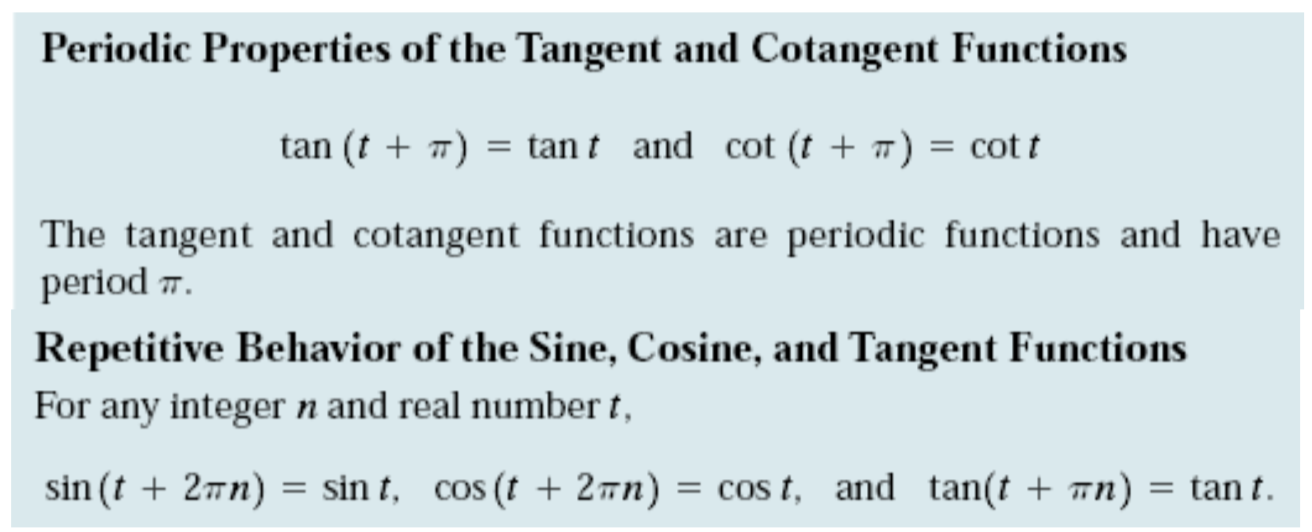
\includegraphics[scale=.6]{periodic}\\

\newpage
\item Given $\displaystyle \sin\Bigg(\frac{\pi}{12}\Bigg)=\frac{\sqrt{6}-\sqrt{2}}{4}$, determine the value of $\displaystyle \sin \Bigg( \frac{49\pi}{12} \Bigg)$.

\vfill
\item Use properties of trigonometric functions to simplify $\tan(-3t)-\tan(-3t+\pi)$.
\vfill

\subsection{Approximate Trigonometric Functions on a Calculator} ~

\item Use a calculator to approximate the function values.  Round to 4 decimal places.
\begin{enumerate}
\item $\displaystyle \cos \Bigg( \frac{2\pi}{7} \Bigg)$\\
\item $\csc(0.92)$\\[.2in]
\end{enumerate}



\end{enumerate}

\noindent \textbf{Student Learning Outcomes Check}

\begin{enumerate}
\item Can you evaluate trigonometric functions using the unit circle?
\item Can you determine domains of trigonometric functions?
\item Are you able to use trigonometric identities?

\end{enumerate}

\noindent \textbf{If any of your answers were no, please ask about these topics in class.}



\actTitle{4.2 - Trigonometric Functions Defined on the Unit Circle}

\noindent \textbf{Topics:}  unit circle, trigonometric functions, trigonometric identities, periodic\\

\noindent \textbf{Student Learning Outcomes:}
\begin{enumerate}
\item Students will be able to evaluate trigonometric functions using the unit circle.
\item Students will be able to determine domains of trigonometric functions.
\item Students will be able to use trigonometric identities.
\end{enumerate}

\hrule 

\bigskip

\subsection{Trigonometric Functions of Real Numbers} ~

\noindent A \textbf{\underline{unit circle}} is a circle of radius 1 with center at the origin.  The equation of a unit circle is:
$$x^2+y^2=1$$

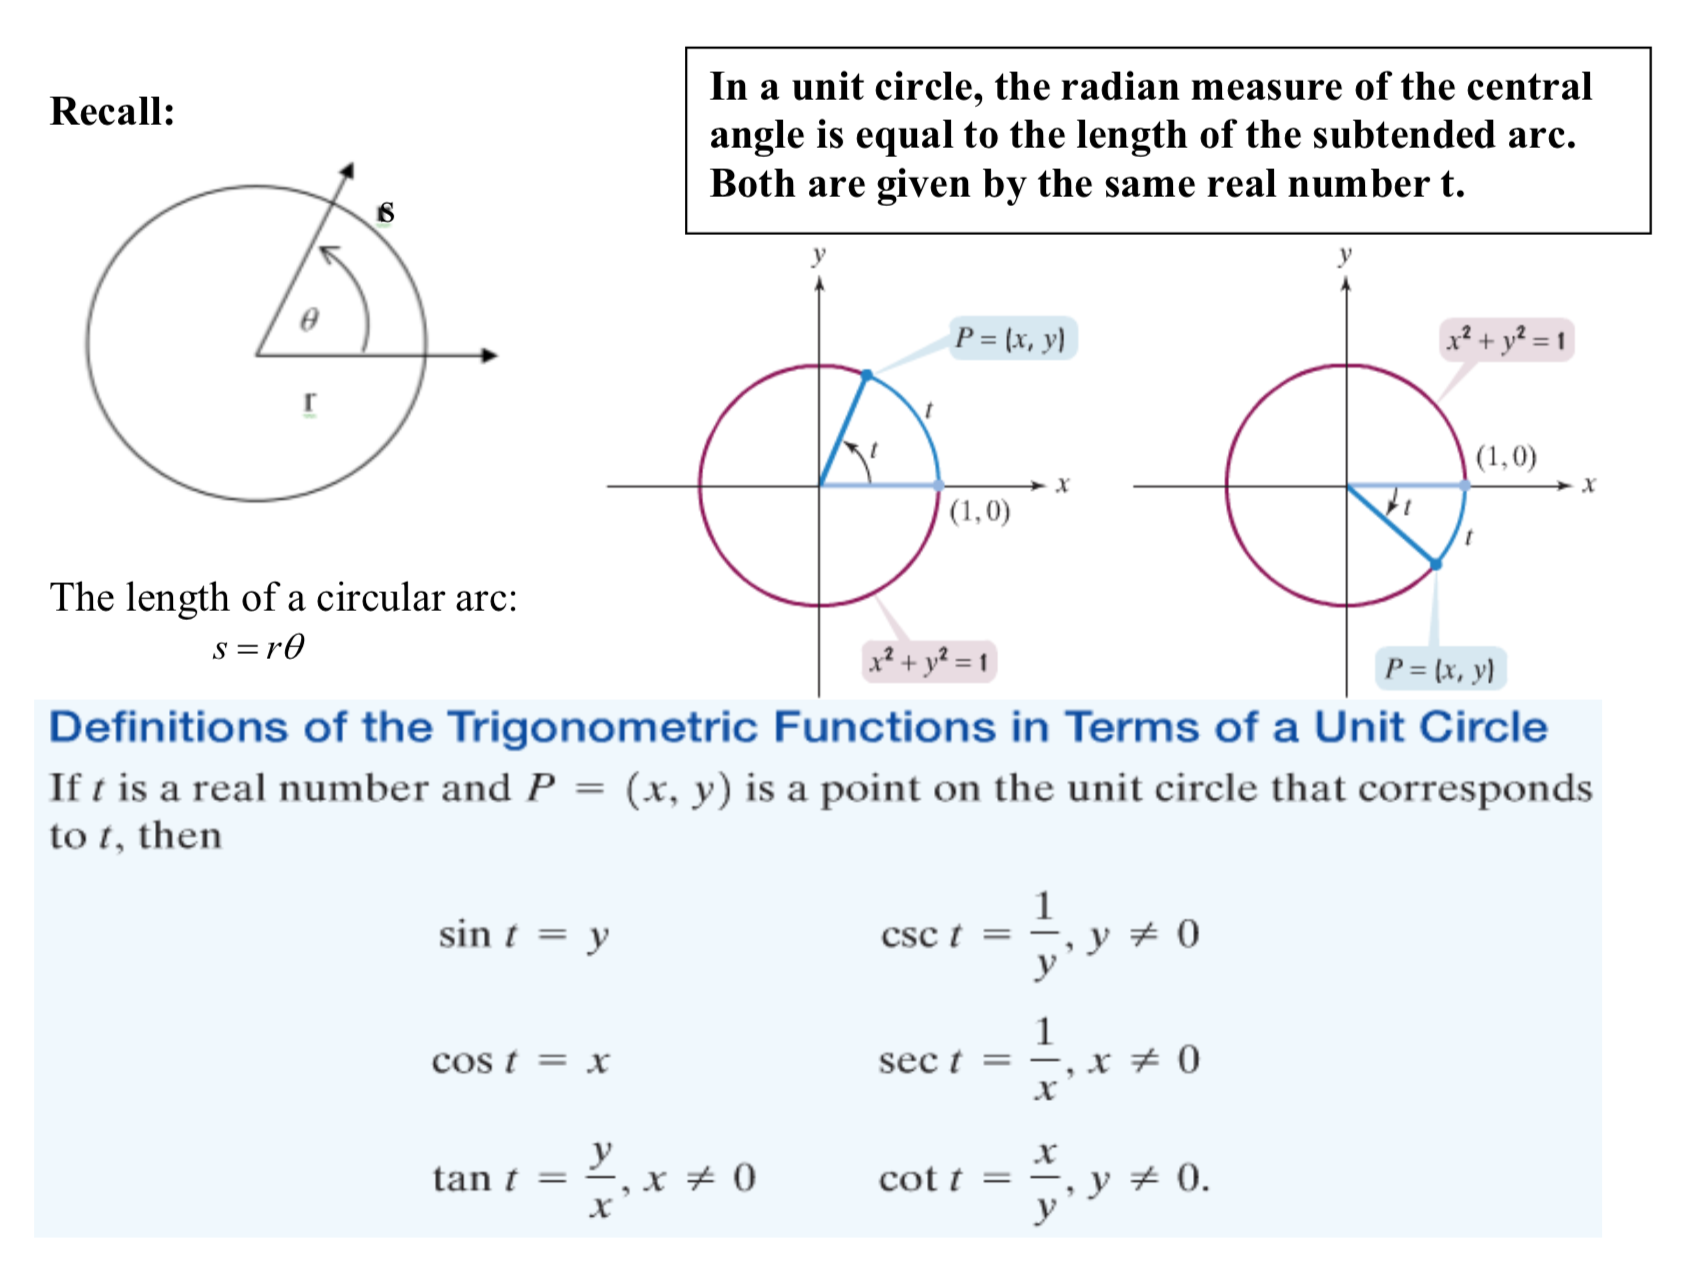
\includegraphics[scale=.6]{unitpic}

\newpage









\begin{enumerate}
\item Suppose that the real number $t$ corresponds to the point $P(-\frac{2}{3},-\frac{\sqrt{5}}{3})$ on the unit circle.  Evaluate the six trigonometric functions of $t$.
\begin{enumerate}
\item $\sin(t)=$\\[.5in]
\item $\cos(t)=$ \\[.5in]
\item $\tan(t)=$ \\[.5in]
\item $\csc(t)=$ \\[.5in]
\item $\sec(t)=$ \\[.5in]
\item $\cot(t)=$ \\[.5in]
\end{enumerate}

\subsection{Fundamental Trigonometric Identities} ~

\textbf{Reciprocal Identities:  }
$$\sin(\theta)=\frac{1}{\csc(\theta)} \quad \quad \cos(\theta)=\frac{1}{\sec(\theta)} \quad \quad \tan(\theta)=\frac{1}{\cot(\theta)}$$
Let's find three more:\\[.2in]

\textbf{Quotient Identities:  }
$$\tan(\theta)=\frac{\sin(\theta)}{\cos(\theta)} \quad \quad \cot(\theta)=\frac{\cos(\theta)}{\sin(\theta)}$$

\item Let $P(\frac{15}{17}, \frac{8}{17})$ be a point on the unit circle that correspond to $t$.  Find each of the six trig functions of $t$.\\[1.7in]

\item Use the $(x,y)$ coordinates in the unit circle to find the value of each trig function at the indicated real number $t$.\\

\begin{enumerate}
\item $\displaystyle \cos\Big(\frac{3\pi}{2}\Big)=$\\[.2in]
\item $\displaystyle \tan\Big(\frac{11\pi}{6}\Big)=$\\[.5in]
\item $\displaystyle \sec\Big(\frac{11\pi}{6}\Big)=$\\[.5in]
\item $\displaystyle \sin(-2\pi)=$\\[.2in]
\end{enumerate}

\item Evaluate the six trigonometric functions of the real number $t$.
\begin{enumerate}
\item $\displaystyle t=\frac{5\pi}{3}$
\newpage
\item $\displaystyle t=-\frac{5\pi}{4}$\vfill
\item $\displaystyle t=\pi$\vfill
\item $\displaystyle t=\frac{5\pi}{2}$\vfill
\end{enumerate}


\newpage

\subsection{Domains of the Trigonometric Functions} ~


\subsubsection{Pythagorean Identities} ~

$$\sin^2(t)+\cos^2(t)=1 \quad \quad \tan^2(t)+1=\sec^2(t) \quad \quad 1+\cot^2(t)=\csc^2(t)$$
\\

\item Given that $\tan(t)=\frac{12}{5}$ for $\pi < t < \frac{3\pi}{2}$, use an appropriate identity to find the value of $\sec(t)$.\\[2in]

\item Given that $\csc(t)=\frac{5}{4}$ for $\frac{\pi}{2} < t < \pi$, use an appropriate identity to find the value of $\cot(t)$.\\[2in]

\item Given a real number $t$, express $\sin(t)$ in terms of $\cos(t)$.\\[1.5in]

\newpage

\subsubsection{Even, Odd, and Periodic Properties} ~

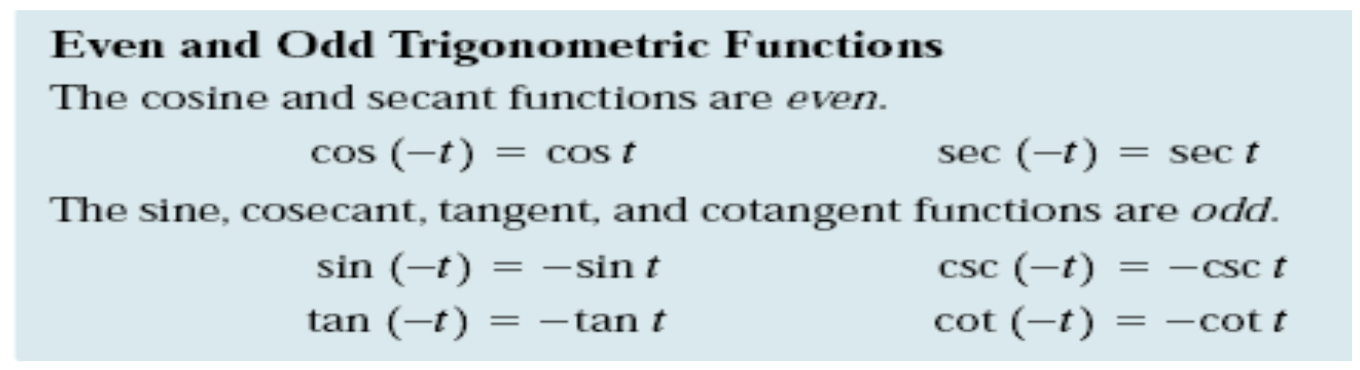
\includegraphics[scale=.6]{evenodd}\\
\item Use the unit circle to find the value of $\displaystyle \cos \Bigg(\frac{2\pi}{3}\Bigg)$ and odd trig functions to find the value of $\displaystyle \cos \Bigg(-\frac{2\pi}{3}\Bigg)$.

\vfill
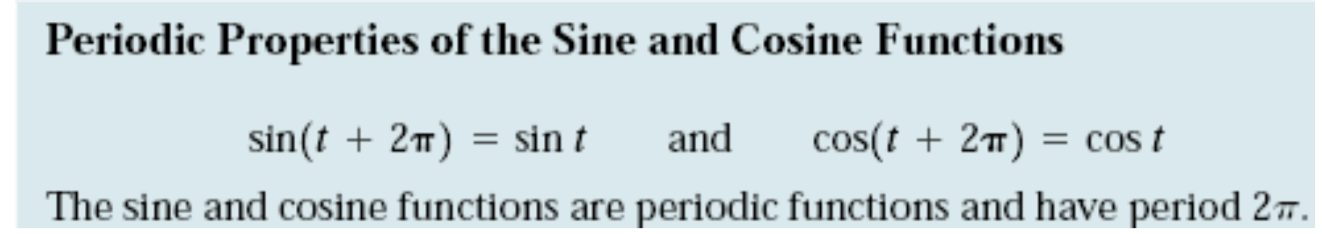
\includegraphics[scale=.6]{periodic1}\\
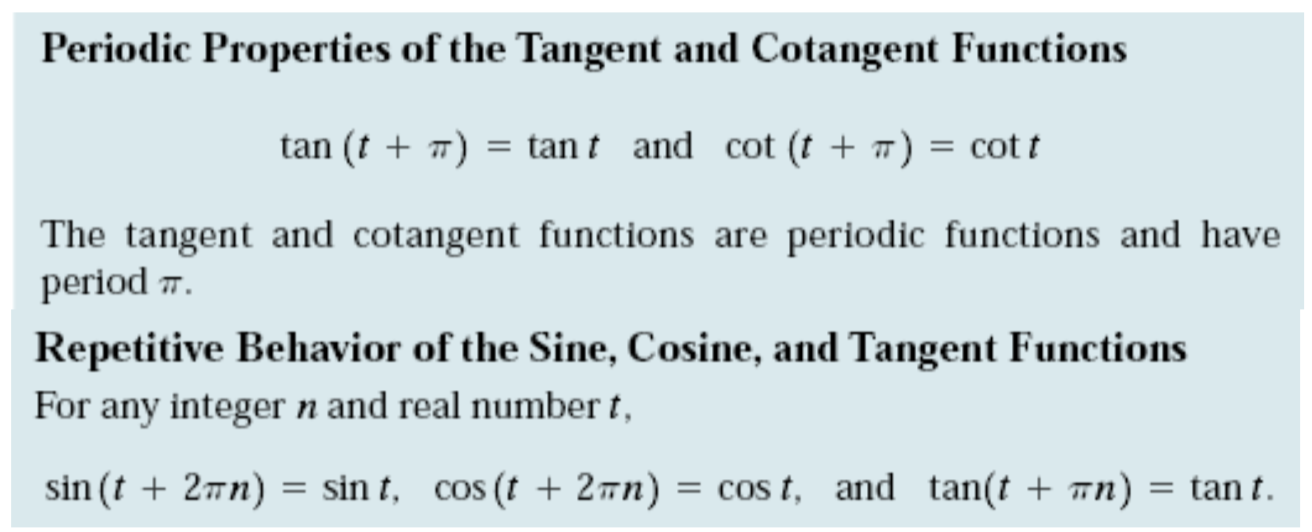
\includegraphics[scale=.6]{periodic}\\

\newpage
\item Given $\displaystyle \sin\Bigg(\frac{\pi}{12}\Bigg)=\frac{\sqrt{6}-\sqrt{2}}{4}$, determine the value of $\displaystyle \sin \Bigg( \frac{49\pi}{12} \Bigg)$.

\vfill
\item Use properties of trigonometric functions to simplify $\tan(-3t)-\tan(-3t+\pi)$.
\vfill

\subsubsection{Approximate Trigonometric Functions on a Calculator} ~

\item Use a calculator to approximate the function values.  Round to 4 decimal places.
\begin{enumerate}
\item $\displaystyle \cos \Bigg( \frac{2\pi}{7} \Bigg)$\\
\item $\csc(0.92)$\\[.2in]
\end{enumerate}



\end{enumerate}

\noindent \textbf{Student Learning Outcomes Check}

\begin{enumerate}
\item Can you evaluate trigonometric functions using the unit circle?
\item Can you determine domains of trigonometric functions?
\item Are you able to use trigonometric identities?

\end{enumerate}

\noindent \textbf{If any of your answers were no, please ask about these topics in class.}



%\documentclass[11pt]{article}
\usepackage{amsmath, amssymb, array}
\pagestyle{plain}

\textwidth=6.5in
\hoffset-1in
\textheight=9in
\voffset-1in

\usepackage{enumitem}
\usepackage{pgfplots}
\usepackage{graphicx}
\usepackage{lipsum}
\usepackage{stfloats}
\usepackage{multicol}
\setlength{\columnsep}{1cm}




\begin{document}


\noindent MATH 1113   \hfill 4.3 - Right Triangle Trigonometry\\



\noindent \textbf{Topics:}  acute angles, right triangle trigonometry, cofunction identities\\

\noindent \textbf{Student Learning Outcomes:}
\begin{enumerate}
\item Students will be able to evaluate trigonometric functions of acute angles.
\item Students will be able to use trigonometric identities.
\item Students will be able to use trigonometric functions in applications.
\end{enumerate}

\hrule 
\vspace{5mm}
\section{Trigonometric Functions of Acute Angles}
\noindent An angle is \textbf{\underline{acute}} if it measures less than 90$^{\circ}$.\\
A \textbf{\underline{right angle}} measures exactly 90$^{\circ}$.\\
The sum of angles of a triangle is 180$^{\circ}$.\\[.2in]

\noindent If we know two sides of a right triangle, we can use the \textbf{Pythagorean Theorem} $a^2+b^2=c^2$ to find the 3rd side.

\begin{center}
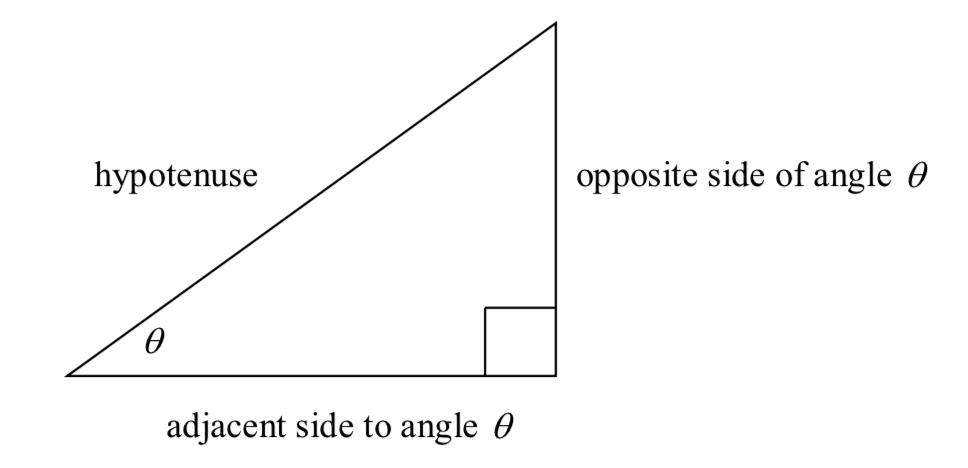
\includegraphics[scale=.6]{righttriangle}\\
\end{center}


In the \textbf{right} triangle above, the \textbf{\emph{six trigonometric functions}} of an angle $\theta$ are defined as follows:

\begin{center}
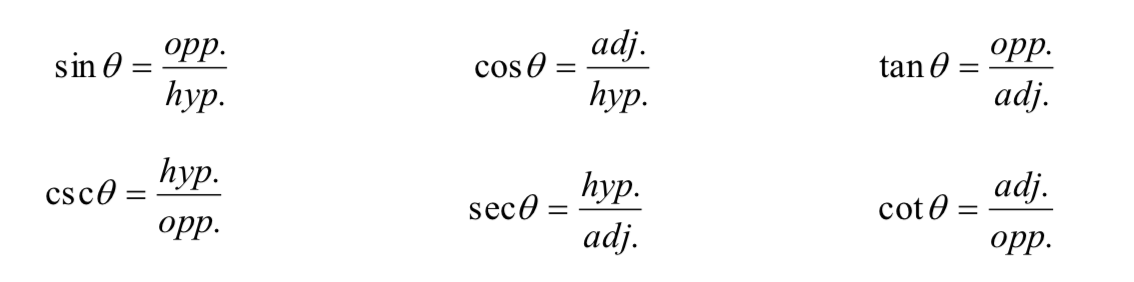
\includegraphics[scale=.6]{trigdef}\\
\end{center}

\newpage





\begin{enumerate}
\item Find the six trig functions of $\theta$ in the triangle below.
\begin{center}
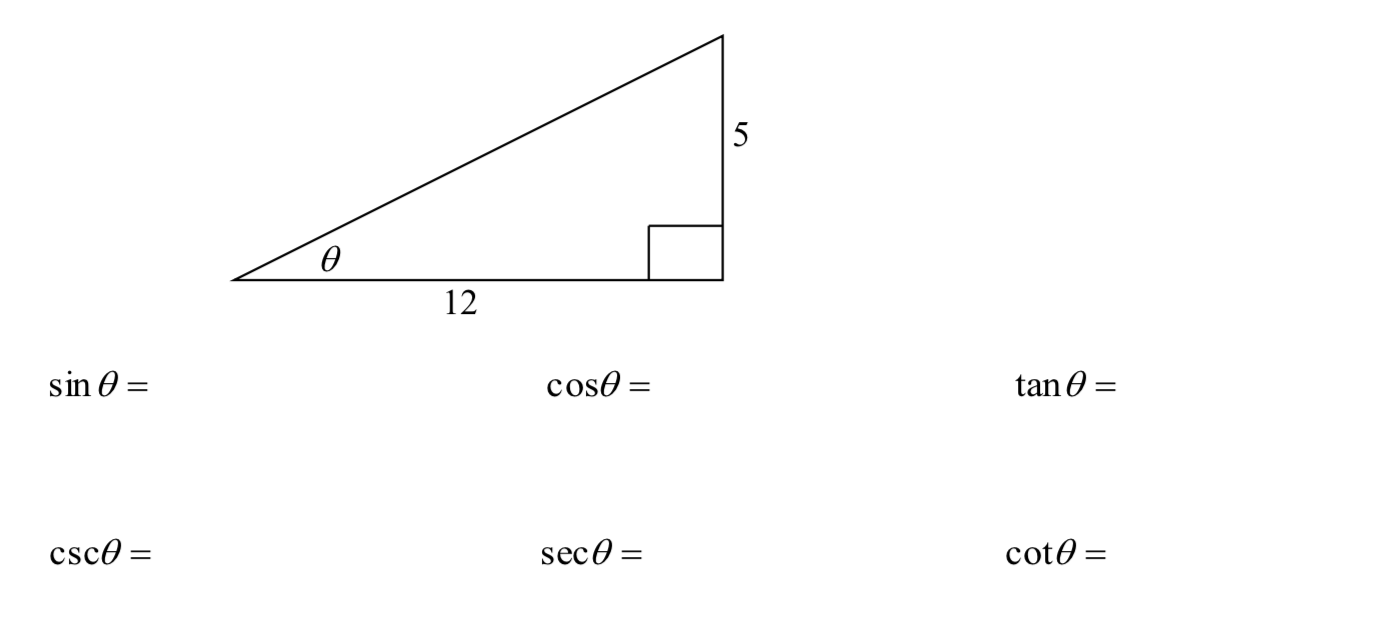
\includegraphics[scale=.6]{trigex1}\\
\end{center}

\item Find the sine, cosine, and tangent of 45$^{\circ}$ using the triangle below.

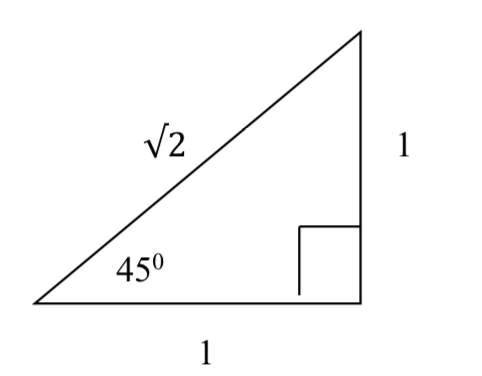
\includegraphics[scale=.6]{trigex2}\\


\item Find the sine, cosine, and tangent of 30$^{\circ}$ and  60$^{\circ}$ using the triangle below.\\
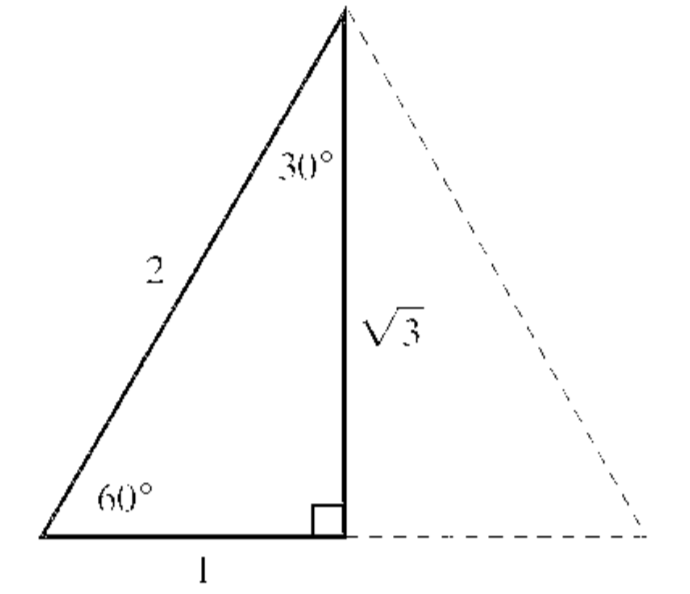
\includegraphics[scale=.6]{trigex3}\\


\newpage

\section{Fundamental Trigonometric Identities}

\textbf{Reciprocal Identities:  }
$$\sin(\theta)=\frac{1}{\csc(\theta)} \quad \quad \cos(\theta)=\frac{1}{\sec(\theta)} \quad \quad \tan(\theta)=\frac{1}{\cot(\theta)}$$
Let's find three more:\\[.2in]

\textbf{Quotient Identities:  }
$$\tan(\theta)=\frac{\sin(\theta)}{\cos(\theta)} \quad \quad \cot(\theta)=\frac{\cos(\theta)}{\sin(\theta)}$$


\item Given $\sin(\theta)=\frac{2}{3}$ and $\cos(\theta)=\frac{\sqrt{5}}{3}$, find the value of each of the four remaining functions.\vfill
\vfill

\newpage
\section{Using Trigonometric Functions in Applications}
\item A forester, 300 feet from the base of a redwood tree, observes that the angle between the ground and the top of the tree is 45$^\circ$.  Determine the height of the tree.

\vfill
\item A pilot flying an airplane at an altitude of 1 mile sights a point at the end of a runway.  The angle of depression is 3$^\circ$.  What is the distance $d$ from the plane to the point on the runway?  Round to the nearest tenth of a mile.
\vfill
\vfill

\newpage
\section{Trigonometric Functions of Real Numbers}
\noindent A \textbf{\underline{unit circle}} is a circle of radius 1 with center at the origin.  The equation of a unit circle is:
$$x^2+y^2=1$$

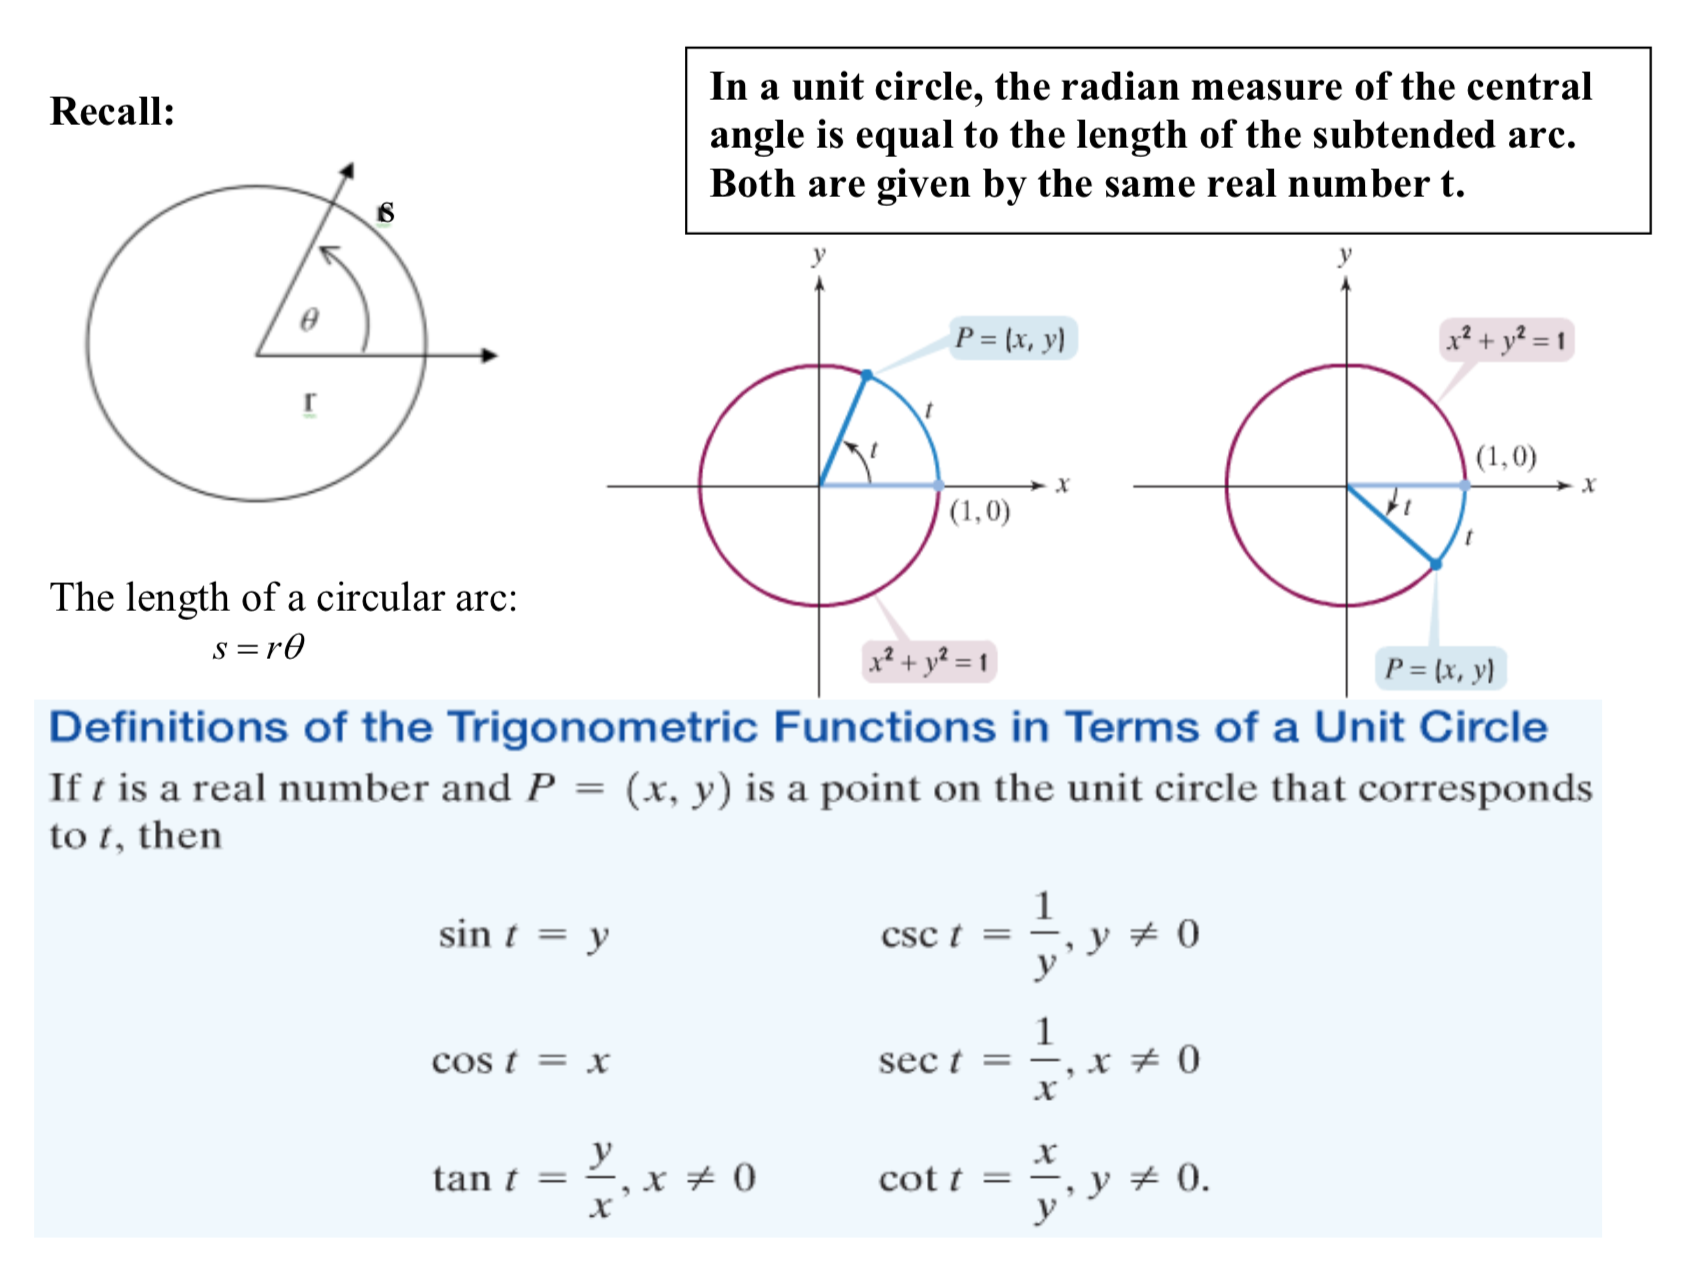
\includegraphics[scale=.6]{unitpic}

\newpage

\item Suppose that the real number $t$ corresponds to the point $P(-\frac{2}{3},-\frac{\sqrt{5}}{3})$ on the unit circle.  Evaluate the six trigonometric functions of $t$.
\begin{enumerate}
\item $\sin(t)=$\\[.5in]
\item $\cos(t)=$ \\[.5in]
\item $\tan(t)=$ \\[.5in]
\item $\csc(t)=$ \\[.5in]
\item $\sec(t)=$ \\[.5in]
\item $\cot(t)=$ \\[.5in]
\end{enumerate}


\item Use the $(x,y)$ coordinates in the unit circle to find the value of each trig function at the indicated real number $t$.\\

\begin{enumerate}
\item $\displaystyle \cos\Big(\frac{3\pi}{2}\Big)=$\\[.2in]
\item $\displaystyle \tan\Big(\frac{11\pi}{6}\Big)=$\\[.5in]
\item $\displaystyle \sec\Big(\frac{11\pi}{6}\Big)=$\\[.5in]

\end{enumerate}

\item Evaluate the six trigonometric functions of the real number $t$.
\begin{enumerate}

\item $\displaystyle t=-\frac{5\pi}{4}$\vfill
\item $\displaystyle t=\pi$\vfill

\end{enumerate}


\newpage

\section{Domains of the Trigonometric Functions}
\vfill



\end{enumerate}





\noindent \textbf{Student Learning Outcomes Check}

\begin{enumerate}
\item Can you evaluate trigonometric functions of acute angles?
\item Are you able to use able to use trigonometric identities?
\item Can you use trigonometric functions in applications?
\end{enumerate}

\noindent \textbf{If any of your answers were no, please ask about these topics in class.}













\end{document}
\actTitle{4.3 - Right Triangle Trigonometry}

\videoLink{Section 4.3}{https://www.youtube.com/playlist?list=PLYHZK3b8UFw2K5Q_epS1Wi1hezUGCYwtP}

\noindent \textbf{Topics:}  acute angles, right triangle trigonometry, cofunction identities\\

\noindent \textbf{Student Learning Outcomes:}
\begin{enumerate}
\item Students will be able to evaluate trigonometric functions of acute angles.
\item Students will be able to use trigonometric identities.
\item Students will be able to use trigonometric functions in applications.
\end{enumerate}

\hrule 

\bigskip

\subsection{Trigonometric Functions of Acute Angles} ~

\noindent An angle is \textbf{\underline{acute}} if it measures less than 90$^{\circ}$.\\
A \textbf{\underline{right angle}} measures exactly 90$^{\circ}$.\\
The sum of angles of a triangle is 180$^{\circ}$.\\[.2in]

\noindent If we know two sides of a right triangle, we can use the
\textbf{Pythagorean Theorem} $a^2+b^2=c^2$ to find the 3rd side.


\begin{center}
  \begin{tikzpicture}[y=1cm, x=1cm,font=\sffamily]
    \draw[black,thick,fill=gray!0] (0,0)--(4,0)--(4,2) -- cycle;
    \draw[black] (3.8,0) -- (3.8,0.2) -- (4,0.2);
    \draw[thin,black] (0.8,0) arc (0:30:0.8)
              node[anchor=west,pos=0.5] {$\theta$};
    \node[anchor=west] at (4,1) {Opposite side of angle $\theta$};
    \node[anchor=north] at (2,0) {Adjacent side of angle $\theta$};
    \node[anchor=south east] at (2,1) {Hypotenuse};
  \end{tikzpicture}
\end{center}

In the \textbf{right} triangle above, the \textbf{\emph{six
    trigonometric functions}} of an angle $\theta$ are defined as
follows:
\begin{eqnarray*}
  \begin{array}{rcl@{\hspace{4em}}rcl@{\hspace{4em}}rcl}
    \sin(\theta) & = & \frac{\textrm{opp.}}{\textrm{hyp.}} & 
    \cos(\theta) & = & \frac{\textrm{adj.}}{\textrm{hyp.}} &
    \tan(\theta) & = & \frac{\textrm{opp.}}{\textrm{adj.}} \\ [10pt]
    \csc(\theta) & = & \frac{\textrm{hyp.}}{\textrm{opp.}} & 
    \sec(\theta) & = & \frac{\textrm{hyp.}}{\textrm{adj.}} &
    \cot(\theta) & = & \frac{\textrm{adj.}}{\textrm{opp.}} 
  \end{array}
\end{eqnarray*}



\newpage





\begin{enumerate}
\item Find the six trig functions of $\theta$ in the triangle below.
  \begin{center}
  \begin{tikzpicture}[y=0.5cm, x=0.5cm,font=\sffamily]
    \draw[black,thick,fill=gray!0] (0,0)--(12,0)--(12,5) -- cycle;
    \draw[black] (11,0) -- (11,1) -- (12,1);
    \draw[thin,black] (2,0) arc (0:24:2)
              node[anchor=west,pos=0.5] {$\theta$};
    \node[anchor=west] at (12,2.5) {5};
    \node[anchor=north] at (6,0) {12};
  \end{tikzpicture}
\end{center}
\begin{eqnarray*}
  \begin{array}{rcl@{\hspace{4em}}rcl@{\hspace{4em}}rcl}
    \sin(\theta) & = &  & 
    \cos(\theta) & = &  &
    \tan(\theta) & = &  \\ [10pt]
    \csc(\theta) & = &  & 
    \sec(\theta) & = &  &
    \cot(\theta) & = & 
  \end{array}
\end{eqnarray*}

\item Find the sine, cosine, and tangent of 45$^{\circ}$ using the triangle below.

  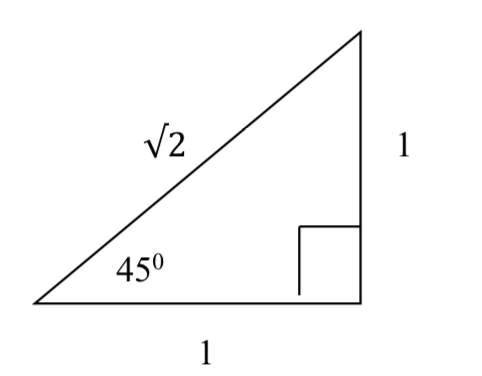
\includegraphics[scale=.6]{trigex2}\\

\item Find the sine, cosine, and tangent of 30$^{\circ}$ and  60$^{\circ}$ using the triangle below.\\
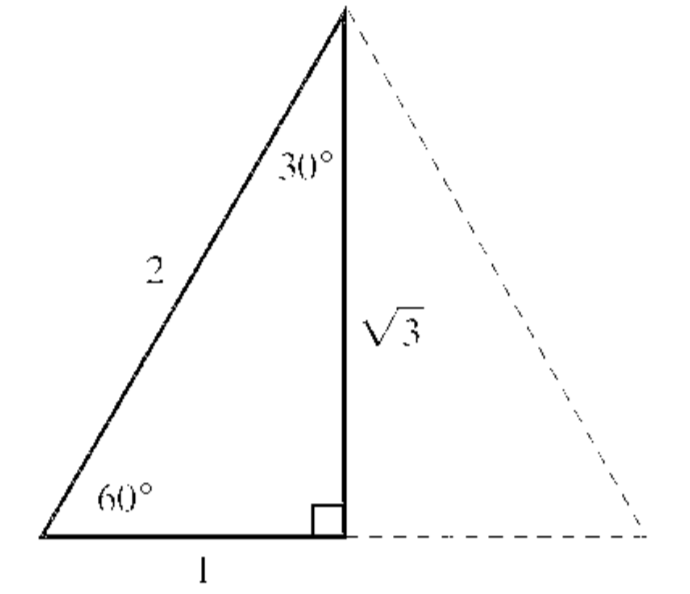
\includegraphics[scale=.6]{trigex3}\\


\newpage

\item Given $\sin(\theta)=\frac{2}{3}$ and $\cos(\theta)=\frac{\sqrt{5}}{3}$, find the value of each of the four remaining functions.\vfill
\vfill


\subsection{Cofunction Identities} ~

\noindent Cofunctions of complementary angles are equal.
$$\sin(\theta)=\cos(90^{\circ}-\theta) \quad \quad \cos(\theta)=\sin(90^{\circ}-\theta)$$
$$\tan(\theta)=\cot(90^{\circ}-\theta) \quad \quad \cot(\theta)=\tan(90^{\circ}-\theta)$$
$$\sec(\theta)=\csc(90^{\circ}-\theta) \quad \quad \csc(\theta)=\sec(90^{\circ}-\theta)$$



\item Fore each function value, find a cofunction with the same value.
\begin{enumerate}
\item $\cot(15^{\circ})=2+\sqrt{3}$\vfill
\item $\displaystyle \cos\Bigg(\frac{\pi}{6}\Bigg)=\frac{\sqrt{3}}{2}$\vfill
\end{enumerate}

\newpage
\subsection{Using Trigonometric Functions in Applications} ~

\item A forester, 300 feet from the base of a redwood tree, observes that the angle between the ground and the top of the tree is 45$^\circ$.  Determine the height of the tree.

\vfill
\item A pilot flying an airplane at an altitude of 1 mile sights a point at the end of a runway.  The angle of depression is 3$^\circ$.  What is the distance $d$ from the plane to the point on the runway?  Round to the nearest tenth of a mile.
\vfill
\vfill
\end{enumerate}

\noindent \textbf{Student Learning Outcomes Check}

\begin{enumerate}
\item Can you evaluate trigonometric functions of acute angles?
\item Are you able to use able to use trigonometric identities?
\item Can you use trigonometric functions in applications?
\end{enumerate}

\noindent \textbf{If any of your answers were no, please ask about these topics in class.}



\actTitle{4.4 - Trigonometric Functions of Any Angle}


\noindent \textbf{Topics:}  increasing and decreasing, reference angles\\

\noindent \textbf{Student Learning Outcomes:}
\begin{enumerate}
\item Students will be able to evaluate trigonometric functions of any angle.
\item Students will be able to determine reference angles.
\item Students will be able to evaluate trigonometric functions using reference angles.
\end{enumerate}

\hrule 

\bigskip

\subsection{Trigonometric Functions of Any Angle} ~

\noindent  Recall:  We have used trigonometric functions with acute angles.  What if the angle is not acute?\vfill

\noindent A circle with center $(0,0)$ and radius $r$ has the equation $x^2+y^2=r^2$.  Choose a point $P(x,y)$.  We can create reference triangles inside the circle in order to define our trig functions.\\[2.5in]


\noindent If the point $(x,y)$ lies on the \textbf{terminal side} of $\theta$, the six trig functions of $\theta$ can be defined as follows:

$$\sin(\theta)=\frac{y}{r} \quad \quad \quad \quad \quad \quad \cos(\theta)=\frac{x}{r} \quad \quad \quad \quad \quad \quad \tan(\theta)=\frac{y}{x} $$

$$\csc(\theta)=\frac{r}{y} \quad \quad \quad \quad \quad \quad \sec(\theta)=\frac{r}{x} \quad \quad \quad \quad \quad \quad \cot(\theta)=\frac{x}{y} $$
\vfill
\noindent What changes when we are on the unit circle?



\newpage



\begin{enumerate}
\item Let $P(-6,8)$ be a point on the terminal side of $\theta$.  Find each of the six trig functions of $\theta$.\\[2in]

\begin{center}
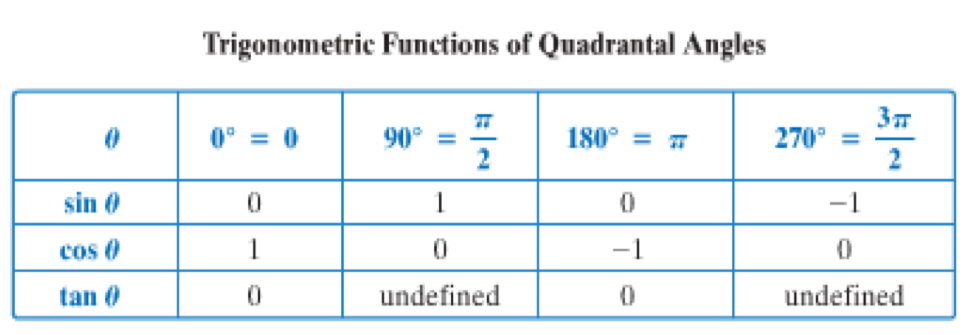
\includegraphics[scale=.7]{quadrantal}
\end{center}

\subsection{The Signs of the Trigonometric Functions} ~

\begin{center}
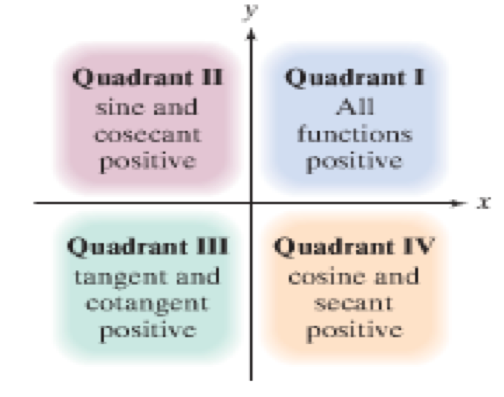
\includegraphics[scale=.8]{signs}
\end{center}

\item Let $\theta$ be an angle in standard position.  Name the quadrant in which $\theta$ lies.
$$\sin(\theta)<0, \quad \quad \tan(\theta)<0$$


\newpage

\item Find the exact value of each of the remaining trigonometric functions of $\theta$.
$$\sin(\theta)=\frac{4}{5}, \quad  \theta \text{ in Quadrant 2}$$\vfill


\subsection{Reference Angles} 

Let's draw our two reference triangles as well as an $xy-$plane.\\[1.5in]
\hspace{-.3in}\begin{tabular}{| l |} \hline
Let $\theta$ be a nonquadrantal angle in standard position. The \underline{reference angle} for $\theta$, \\ called $\theta_R$, is the \emph{acute} angle $\theta_R$ that the \emph{terminal side} of $\theta$ makes with the $x$-axis. \\ \hline
\end{tabular}\\
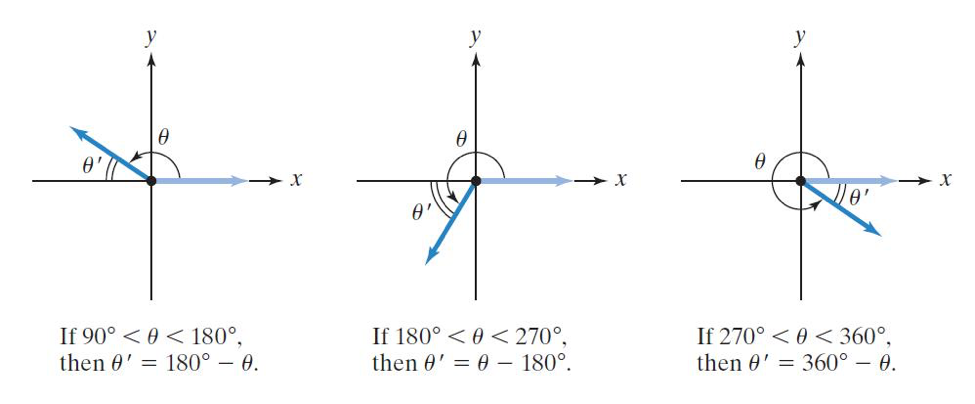
\includegraphics{refimage}\\

\newpage

\item Determine the reference angle $\theta_R$ for each of the following angles.
\begin{enumerate}
\item $\theta = 45^\circ$ \hspace{1in} Quadrant \underline{\phantom{sldkjfslkdjf}} \hspace{1in} $\theta_R$ \underline{\phantom{sldkjfslkdjf}} \\[.8in]
\item $\theta = -73^\circ$ \hspace{1in} Quadrant \underline{\phantom{sldkjfslkdjf}} \hspace{1in} $\theta_R$ \underline{\phantom{sldkjfslkdjf}}  \\[.8in]

\item $\theta = -915^\circ$ \hspace{1in} Quadrant \underline{\phantom{sldkjfslkdjf}} \hspace{1in} $\theta_R$ \underline{\phantom{sldkjfslkdjf}}  \\[.8in]

\end{enumerate}

\item Determine the reference angle $\theta_R$ for each of the following angles. 
\begin{enumerate}

\item $\theta = \dfrac{19\pi}{6}$ \hspace{1in} Quadrant \underline{\phantom{sldkjfslkdjf}} \hspace{1in} $\theta_R$ \underline{\phantom{sldkjfslkdjf}} \vfill
\item $\theta = \dfrac{47\pi}{4}$ \hspace{1in} Quadrant \underline{\phantom{sldkjfslkdjf}} \hspace{1in} $ \theta_R$ \underline{\phantom{sldkjfslkdjf}} \vfill
\item $\theta = \dfrac{-7\pi}{6}$ \hspace{1in} Quadrant \underline{\phantom{sldkjfslkdjf}} \hspace{1in} $\theta_R$ \underline{\phantom{sldkjfslkdjf}} \vfill

\end{enumerate}

\newpage


\hspace{-.3in}\begin{tabular}{| l |} \hline
Let $\theta$ be a nonquadrantal angle in standard position. To find the value of a trig function\\ at $\theta$, find its value for the \emph{reference angle} $\theta_R$ and prefix the appropriate sign (using ASTC). \\ \hline
\end{tabular}

\item Determine the exact values of $\sin(2\pi/3)$ and $\cos(2\pi/3)$. \\[1.5in] %QII


\item Determine the exact values of $\cos(210^\circ)$, $\sec(210^\circ)$, and $\cot(210^\circ)$. \\[1.5in]
\vfill
%
%\item Determine the exact value of each of the following. %same ref
%\begin{enumerate}
%\item $\sin(7\pi/6)$ \vfill
%
%\item $\sin(11\pi/6)$ \vfill
%\item $\sin(5\pi/6)$ \vfill
%\end{enumerate}
%
%
%\newpage
%\item Suppose $\theta$ is an angle in the third quadrant with reference angle $\theta_R$ satisfying $\cos(\theta_R)=5/13$ and $\sin(\theta_R)=12/13$.  Determine the exact values of $\cos(\theta)$ and $\csc(\theta)$.  \vfill


\end{enumerate}

\noindent \textbf{Student Learning Outcomes Check}

\begin{enumerate}
\item Can you evaluate trigonometric functions of any angle?
\item Are you able to determine reference angles?
\item Can you evaluate trigonometric functions using reference angles?
\end{enumerate}

\noindent \textbf{If any of your answers were no, please ask about these topics in class.}



%\actTitle{4.4 - Trigonometric Functions of Any Angle}

\videoLink{Section 4.4}{https://www.youtube.com/playlist?list=PLYHZK3b8UFw2OmnPlWMPeyRScOjE2Rk4C}

\noindent \textbf{Topics:}  increasing and decreasing, reference angles\\

\noindent \textbf{Student Learning Outcomes:}
\begin{enumerate}
\item Students will be able to evaluate trigonometric functions of any angle.
\item Students will be able to determine reference angles.
\item Students will be able to evaluate trigonometric functions using reference angles.
\end{enumerate}

\hrule 

\bigskip

\subsection{Trigonometric Functions of Any Angle} ~

\noindent  Recall:  We have used trigonometric functions with acute angles.  What if the angle is not acute?\vfill

\noindent A circle with center $(0,0)$ and radius $r$ has the equation $x^2+y^2=r^2$.  Choose a point $P(x,y)$.  We can create reference triangles inside the circle in order to define our trig functions.\\[2.5in]


\noindent If the point $(x,y)$ lies on the \textbf{terminal side} of $\theta$, the six trig functions of $\theta$ can be defined as follows:

$$\sin(\theta)=\frac{y}{r} \quad \quad \quad \quad \quad \quad \cos(\theta)=\frac{x}{r} \quad \quad \quad \quad \quad \quad \tan(\theta)=\frac{y}{x} $$

$$\csc(\theta)=\frac{r}{y} \quad \quad \quad \quad \quad \quad \sec(\theta)=\frac{r}{x} \quad \quad \quad \quad \quad \quad \cot(\theta)=\frac{x}{y} $$
\vfill
\noindent What changes when we are on the unit circle?



\newpage



\begin{enumerate}
\item Let $P(-6,8)$ be a point on the terminal side of $\theta$.  Find each of the six trig functions of $\theta$.\\[2in]

\begin{center}
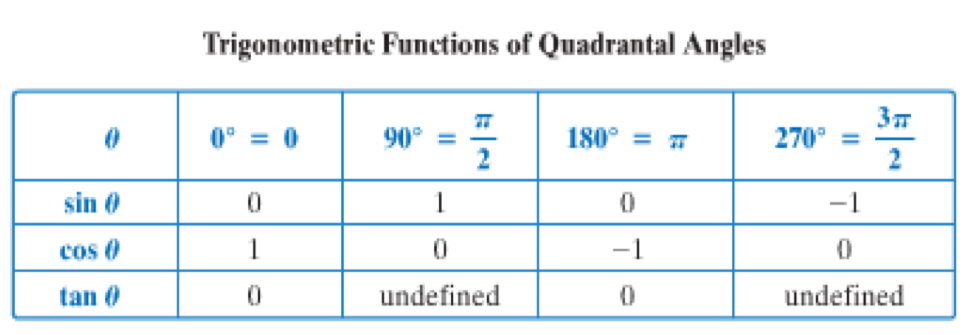
\includegraphics[scale=.7]{quadrantal}
\end{center}

\subsection{The Signs of the Trigonometric Functions} ~

\begin{center}
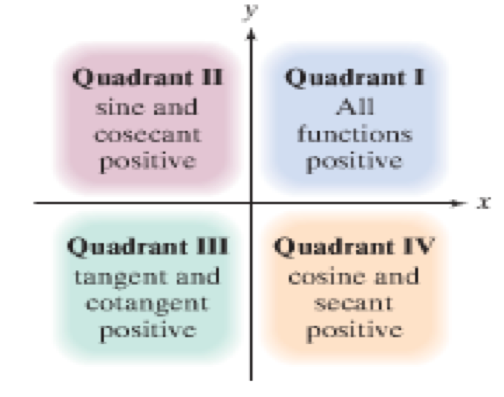
\includegraphics[scale=.8]{signs}
\end{center}

\item Let $\theta$ be an angle in standard position.  Name the quadrant in which $\theta$ lies.
$$\sin(\theta)<0, \quad \quad \tan(\theta)<0$$


\newpage

\item Find the exact value of each of the remaining trigonometric functions of $\theta$.
$$\sin(\theta)=\frac{4}{5}, \quad  \theta \text{ in Quadrant 2}$$\vfill


\subsection{Reference Angles}

Let's draw our two reference triangles as well as an $xy-$plane.\\[1.5in]
\hspace{-.3in}\begin{tabular}{| l |} \hline
Let $\theta$ be a nonquadrantal angle in standard position. The \underline{reference angle} for $\theta$, \\ called $\theta_R$, is the \emph{acute} angle $\theta_R$ that the \emph{terminal side} of $\theta$ makes with the $x$-axis. \\ \hline
\end{tabular}\\
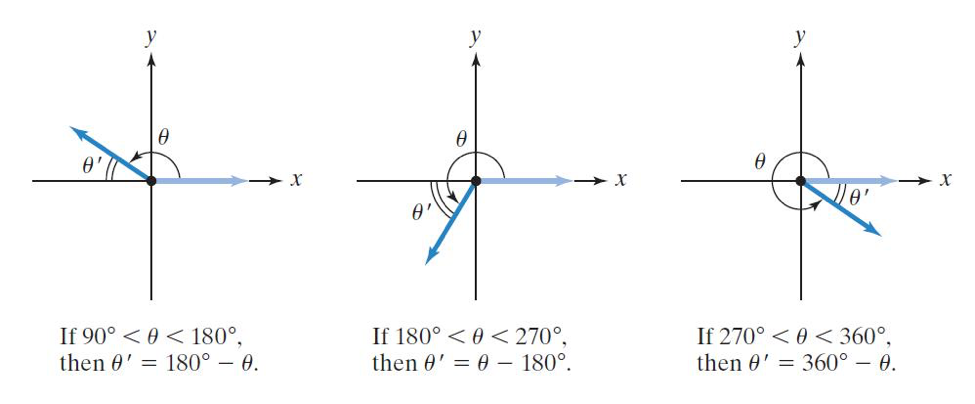
\includegraphics{refimage}\\

\newpage

\item Determine the reference angle $\theta_R$ for each of the following angles.
\begin{enumerate}
\item $\theta = 45^\circ$ \hspace{1in} Quadrant \underline{\phantom{sldkjfslkdjf}} \hspace{1in} $\theta_R$ \underline{\phantom{sldkjfslkdjf}} \\[.8in]
\item $\theta = -73^\circ$ \hspace{1in} Quadrant \underline{\phantom{sldkjfslkdjf}} \hspace{1in} $\theta_R$ \underline{\phantom{sldkjfslkdjf}}  \\[.8in]

\item $\theta = -915^\circ$ \hspace{1in} Quadrant \underline{\phantom{sldkjfslkdjf}} \hspace{1in} $\theta_R$ \underline{\phantom{sldkjfslkdjf}}  \\[.8in]

\end{enumerate}

\item Determine the reference angle $\theta_R$ for each of the following angles. 
\begin{enumerate}

\item $\theta = \dfrac{19\pi}{6}$ \hspace{1in} Quadrant \underline{\phantom{sldkjfslkdjf}} \hspace{1in} $\theta_R$ \underline{\phantom{sldkjfslkdjf}} \vfill
\item $\theta = \dfrac{47\pi}{4}$ \hspace{1in} Quadrant \underline{\phantom{sldkjfslkdjf}} \hspace{1in} $ \theta_R$ \underline{\phantom{sldkjfslkdjf}} \vfill
\item $\theta = \dfrac{-7\pi}{6}$ \hspace{1in} Quadrant \underline{\phantom{sldkjfslkdjf}} \hspace{1in} $\theta_R$ \underline{\phantom{sldkjfslkdjf}} \vfill

\end{enumerate}

\newpage


\hspace{-.3in}\begin{tabular}{| l |} \hline
Let $\theta$ be a nonquadrantal angle in standard position. To find the value of a trig function\\ at $\theta$, find its value for the \emph{reference angle} $\theta_R$ and prefix the appropriate sign (using ASTC). \\ \hline
\end{tabular}

\item Determine the exact values of $\sin(2\pi/3)$ and $\cos(2\pi/3)$. \\[1.5in] %QII


\item Determine the exact values of $\cos(210^\circ)$, $\sec(210^\circ)$, and $\cot(210^\circ)$. \\[1.5in]
\vfill
%
%\item Determine the exact value of each of the following. %same ref
%\begin{enumerate}
%\item $\sin(7\pi/6)$ \vfill
%
%\item $\sin(11\pi/6)$ \vfill
%\item $\sin(5\pi/6)$ \vfill
%\end{enumerate}
%
%
%\newpage
%\item Suppose $\theta$ is an angle in the third quadrant with reference angle $\theta_R$ satisfying $\cos(\theta_R)=5/13$ and $\sin(\theta_R)=12/13$.  Determine the exact values of $\cos(\theta)$ and $\csc(\theta)$.  \vfill


\end{enumerate}

\noindent \textbf{Student Learning Outcomes Check}

\begin{enumerate}
\item Can you evaluate trigonometric functions of any angle?
\item Are you able to determine reference angles?
\item Can you evaluate trigonometric functions using reference angles?
\end{enumerate}

\noindent \textbf{If any of your answers were no, please ask about these topics in class.}


\actTitle{4.5 - Graphs of Sine and Cosine Functions}

\videoLink{Section 4.5 day 1}{https://www.youtube.com/playlist?list=PLYHZK3b8UFw0U_iMosD8HZraus76s5k2i}
% \videoLink{Section 4.5 day 2}{https://www.youtube.com/playlist?list=PLYHZK3b8UFw0U_iMosD8HZraus76s5k2i}

\noindent \textbf{Topics:}  graphs of $a\sin(bx+c)$ and $a\cos(bx+c)$, period, amplitude, and phase shift\\

\noindent \textbf{Student Learning Outcomes:}
\begin{enumerate}
\item Students will be able to graph $a\sin(bx+c)$ and $a\cos(bx+c)$.
\item Students will be able to determine a sine and cosine wave given a written description.
\item Students will be able to determine the formula for a sine or cosine wave given the graph of the function.
\end{enumerate}

\hrule 

\bigskip

\subsection{Graph $y=\sin(x)$ and $y=\cos(x)$} ~


\noindent
  \begin{tikzpicture}[y=1.0cm, x=0.8cm,font=\sffamily]
    \begin{scope}
      %% ticks
      % \draw[step = 1.0, gray,dashed] (-3,-1.2) grid (3,1.2);
      %% axis
      \draw[thick,->] (-4.5,0) -- coordinate (x axis mid) (8.5,0)
           node[anchor = north west,xshift=-4] {$x$};
      \draw[thick,->] (0,-1.5) -- coordinate (y axis mid) (0,1.5)
           node[anchor = north west] {$y$};
      \foreach \y in {-1,1} {
        \draw (1pt, \y) -- (-1pt, \y) node[anchor=east] {\y};
      }
      \foreach \x in {-4,-3,...,8} {
        \draw(\x,4pt) -- (\x,-4pt);
      }

      \node[yshift=-5,xshift=0,anchor=north] at (1,0) {$\frac{\pi}{2}$};
      \node[yshift=-5,xshift=0,anchor=north] at (2,0) {$\pi$};
      \foreach \x in {3,5,7} {
        \node[yshift=-5,xshift=0,anchor=north] at (\x,0) {$\frac{\x\pi}{2}$};
      }
      \foreach \x in {2,3,4} {
        \node[yshift=-5,xshift=2.5,anchor=north] at (2*\x,0) {$\x\pi$};
      }

      \node[yshift=-5,xshift=0,anchor=north] at (-1,0)  {$-\frac{\pi}{2}$};
      \node[yshift=-5,xshift=-5,anchor=north] at (-2,0) {$-\pi$};
      \node[yshift=-5,xshift=0,anchor=north] at (-3,0)  {$-\frac{3\pi}{2}$};
      \node[yshift=-5,xshift=-10,anchor=north] at (-4,0) {$-2\pi$};

      \draw[black] (4,-0.6) -- (4,-1.5);
      \draw[black,<-] (0,-1.3) -- (1.2,-1.3);
      \draw[black,->] (2.8,-1.3) -- (4,-1.3);
      \node[black,align=center,text width=5em,font=\scriptsize,yshift=-5] at (2,-1.3)
           {1 cycle, period$=2\pi$};

      \draw[black] (-1.3,-1) -- (-5.5,-1);
      \draw[black] (-3.1, 1) -- (-5.5, 1);
      \draw[black,->] (-5.5, 0.4) -- (-5.5,1);
      \draw[black,<-] (-5.5,-0.4) -- (-5.5,-1);
      \node[black,align=center,text width=5em,font=\scriptsize,xshift=-5] at (-5.5,0)
         {Range is $-1\leq y \leq 1$};

      \begin{scope}
        %% \clip(-4,-1) rectangle (8,5);
        \draw[scale=1.0,domain=-4.5:8.5,smooth,variable=\x,very thick,blue!50!black,samples=120,<->]
           plot ({\x},{sin(deg(0.5*pi*\x))}) node[anchor=east] {$\sin(x)$};
      \end{scope}
    \end{scope}

    \begin{scope}[shift={(10,0)},scale=1.0]
      \fill [red!10!white] (-1.1,-1.8) rectangle (5.5,1.5);
      \draw[thick,->] (-0.8,0) -- coordinate (x axis mid) (4.5,0)
           node[anchor = north west] {$x$};
      \draw[thick,->] (-0.4,-1.2) -- coordinate (y axis mid) (-0.4,1.2)
           node[anchor = north east] {$y$};
      \begin{scope}
        %% \clip(-4,-1) rectangle (8,5);
        \draw[scale=1.0,domain=0:4,smooth,variable=\x,very thick,blue!50!black,samples=60,<->]
           plot ({\x},{sin(deg(0.5*pi*\x))});
      \end{scope}
      \node[anchor=south,font=\scriptsize,blue] at (1,1) {$A\sin(Bx-C)$};   
      \draw[black] (0,-0.3) -- (0,-1.7);
      \draw[black] (4,-0.3) -- (4,-1.7);
      \draw[black,<-] (0,-1.5) -- (0.8,-1.5);
      \draw[black,->] (3.2,-1.5) -- (4,-1.5);
      \node[black,align=center,text width=5em,font=\scriptsize,yshift=0] at (2,-1.5)
           {Period$=\frac{2\pi}{B}$};
      \node[black,align=center,text width=3em,font=\scriptsize,xshift=-2,anchor=north west] at (0,0)
           {Starting point: $x=\frac{C}{B}$};

      \draw[black] (1.3,1) -- (3.5,1);
      \draw[black,->] (3.3, 0.7) -- (3.3,1);
      \draw[black,<-] (3.3, 0.0) -- (3.3,0.3);
      \node[black,align=center,text width=3em,font=\scriptsize,xshift=0] at (3.3,0.5)
          {Amplitude: $|A|$};
    \end{scope}
  \end{tikzpicture}

\noindent
  \begin{tikzpicture}[y=1.0cm, x=0.8cm,font=\sffamily]
    \begin{scope}
      %% ticks
      % \draw[step = 1.0, gray,dashed] (-3,-1.2) grid (3,1.2);
      %% axis
      \draw[thick,->] (-4.5,0) -- coordinate (x axis mid) (8.5,0)
           node[anchor = north west,xshift=-4] {$x$};
      \draw[thick,->] (0,-1.5) -- coordinate (y axis mid) (0,1.5)
           node[anchor = north west] {$y$};
      \foreach \y in {-1,1} {
        \draw (1pt, \y) -- (-1pt, \y) node[anchor=east] {\y};
      }
      \foreach \x in {-4,-3,...,8} {
        \draw(\x,4pt) -- (\x,-4pt);
      }

      \node[yshift=-5,xshift=0,anchor=north] at (1,0) {$\frac{\pi}{2}$};
      \node[yshift=-5,xshift=0,anchor=north] at (2,0) {$\pi$};
      \foreach \x in {3,5,7} {
        \node[yshift=-5,xshift=0,anchor=north] at (\x,0) {$\frac{\x\pi}{2}$};
      }
      \foreach \x in {2,3,4} {
        \node[yshift=-5,xshift=2.5,anchor=north] at (2*\x,0) {$\x\pi$};
      }

      \node[yshift=-5,xshift=0,anchor=north] at (-1,0)  {$-\frac{\pi}{2}$};
      \node[yshift=-5,xshift=-5,anchor=north] at (-2,0) {$-\pi$};
      \node[yshift=-5,xshift=0,anchor=north] at (-3,0)  {$-\frac{3\pi}{2}$};
      \node[yshift=-5,xshift=-10,anchor=north] at (-4,0) {$-2\pi$};

      \draw[black] (4,-0.6) -- (4,-1.5);
      \draw[black] (4,0.3) -- (4,0.9);
      \draw[black,<-] (0,-1.3) -- (1.2,-1.3);
      \draw[black,->] (2.8,-1.3) -- (4,-1.3);
      \node[black,align=center,text width=5em,font=\scriptsize,yshift=-5] at (2,-1.3)
           {1 cycle, period$=2\pi$};

      \draw[black] (-2.3,-1) -- (-5.5,-1);
      \draw[black] (-4.4, 1) -- (-5.5, 1);
      \draw[black,->] (-5.5, 0.4) -- (-5.5,1);
      \draw[black,<-] (-5.5,-0.4) -- (-5.5,-1);
      \node[black,align=center,text width=5em,font=\scriptsize,xshift=-5] at (-5.5,0)
         {Range is $-1\leq y \leq 1$};

      \begin{scope}
        %% \clip(-4,-1) rectangle (8,5);
        \draw[scale=1.0,domain=-4.5:8.5,smooth,variable=\x,very thick,blue!50!black,samples=120,<->]
           plot ({\x},{cos(deg(0.5*pi*\x))}) node[anchor=south east,yshift=4] {$\cos(x)$};
      \end{scope}
    \end{scope}

    \begin{scope}[shift={(10,0)},scale=1.0]
      \fill [red!10!white] (-1.1,-1.8) rectangle (5.5,1.5);
      \draw[thick,->] (-0.8,0) -- coordinate (x axis mid) (4.5,0)
           node[anchor = north west] {$x$};
      \draw[thick,->] (-0.4,-1.2) -- coordinate (y axis mid) (-0.4,1.2)
           node[anchor = north east] {$y$};
      \begin{scope}
        %% \clip(-4,-1) rectangle (8,5);
        \draw[scale=1.0,domain=0:4,smooth,variable=\x,very thick,blue!50!black,samples=60,<->]
           plot ({\x},{cos(deg(0.5*pi*\x))});
      \end{scope}
      \node[anchor=south,font=\scriptsize,blue] at (1,1) {$A\cos(Bx-C)$};   
      \draw[black] (0,-0.3) -- (0,-1.7);
      \draw[black] (4,-0.3) -- (4,-1.7);
      \draw[black,<-] (0,-1.5) -- (0.8,-1.5);
      \draw[black,->] (3.2,-1.5) -- (4,-1.5);
      \node[black,align=center,text width=5em,font=\scriptsize,yshift=0] at (2,-1.5)
           {Period$=\frac{2\pi}{B}$};
      \node[black,align=center,text width=3em,font=\scriptsize,xshift=-2,anchor=north west] at (-0.2,0)
           {Starting point: $x=\frac{C}{B}$};

      \draw[black] (0.5,1) -- (2.2,1);
      \draw[black,->] (2.0, 0.7) -- (2.0,1);
      \draw[black,<-] (2.0, 0.0) -- (2.0,0.3);
      \node[black,align=center,text width=3em,font=\scriptsize,xshift=0] at (2.0,0.5)
          {Amplitude: $|A|$};
    \end{scope}
  \end{tikzpicture}


  \noindent \underline{Recall} The period of the sine graph is $2\pi$;
  the period of the cosine graph is also $2\pi$.


\begin{enumerate}
\vspace{-.1in}
\item \begin{enumerate} \item Explain how to obtain the graph of $f(x)=-3\sin(x)$ from the graph of $y=\sin(x)$.\\[.5in]
\item Sketch the graph of the function $f(x)= -3\sin(x)$. \\
\scalebox{.8}{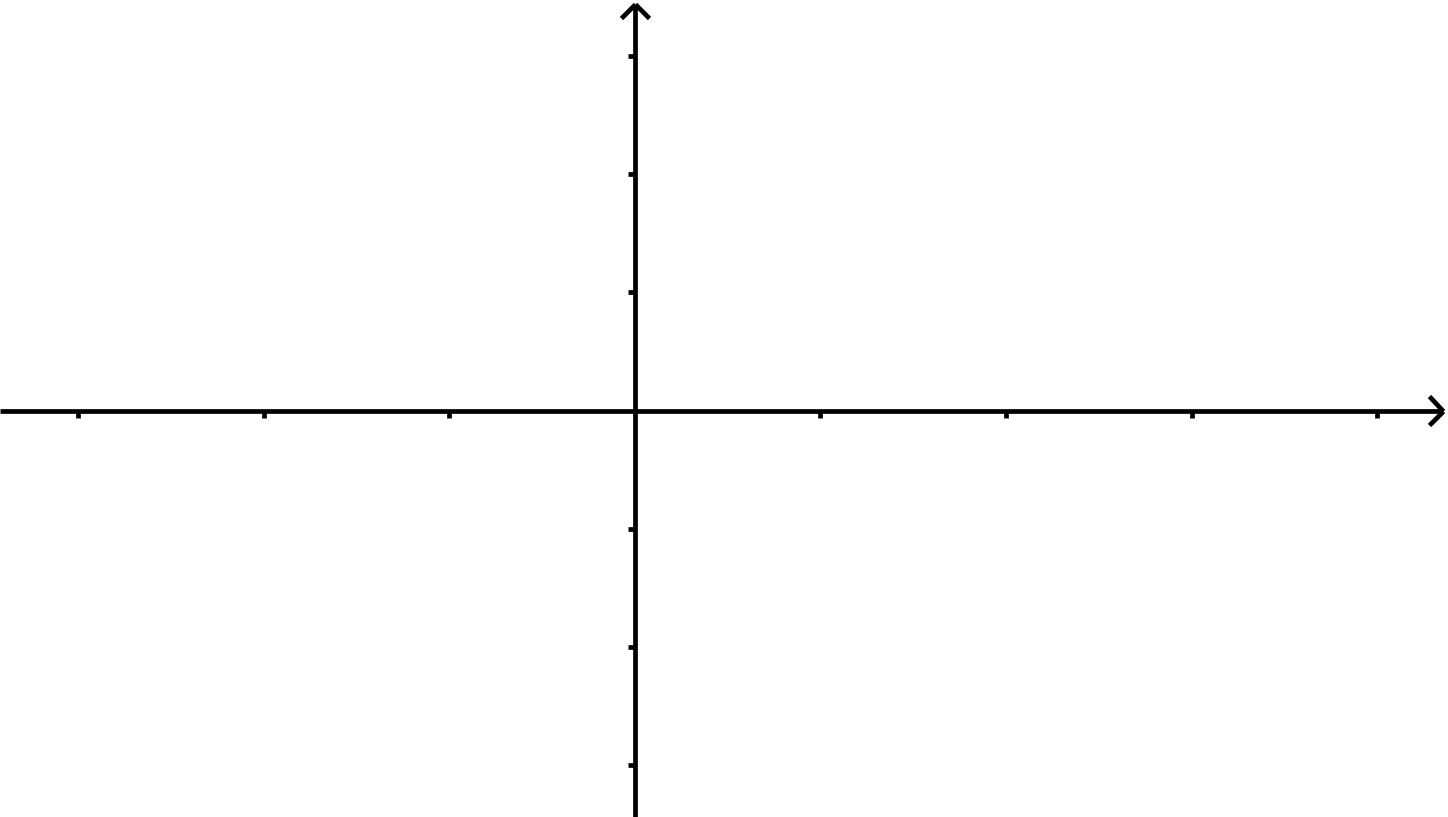
\includegraphics[scale=1.5]{gentrig1}}\\
\item Determine the period and amplitude of the function $f(x)= -3\sin(x)$. \\[1in]
\end{enumerate}



\hspace{-.3in} \begin{tabular}{| l | }
\hline 
For a function $y=A\sin(Bx+C)$ or $y=A \cos(Bx+C)$, assuming that $A$ and $B$ are both not zero, \\

$\star$ The \emph{amplitude} is $|A|$.\\
$\star$ The \emph{period} is $2\pi/|B|$.   \\
$\star$ The \emph{phase shift} is $-C/B$. A negative phase shift is a shift to the left; a positive phase shift\\ is a shift to the right. You can get it from graph transformations if you do the horizontal shift \emph{last}.% \\
%$\star$ To find an interval containing exactly one cycle, solve the equations $0=bx+c$ and $2\pi = bx+c$. 
\\ \hline
\end{tabular}

\vfill
\textbf{How to Graph Sine and Cosine Functions}
\begin{enumerate}
\item Find amplitude, period, and phase shift.
\item Determine the interval of one period on the $x$-axis. (Set interval $0\leq Bx+C \leq 2\pi$ and solve.
\item Divide the interval into fourths to plot "key points".
\item Use rules for function transformation.
\end{enumerate}
\vfill


\newpage

\item \begin{enumerate} \item Explain how to obtain the graph of $f(x)=\sin(x+\pi/6)$ from the graph of $y=\sin(x)$. \\[.75in]

\item Determine the period, amplitude, and phase shift.\\[1.5in]

\item Find an interval containing exactly one cycle.\vfill

\item Sketch the graph of $f(x)=\sin(x+\pi/6)$. 
\end{enumerate} 

\scalebox{.8}{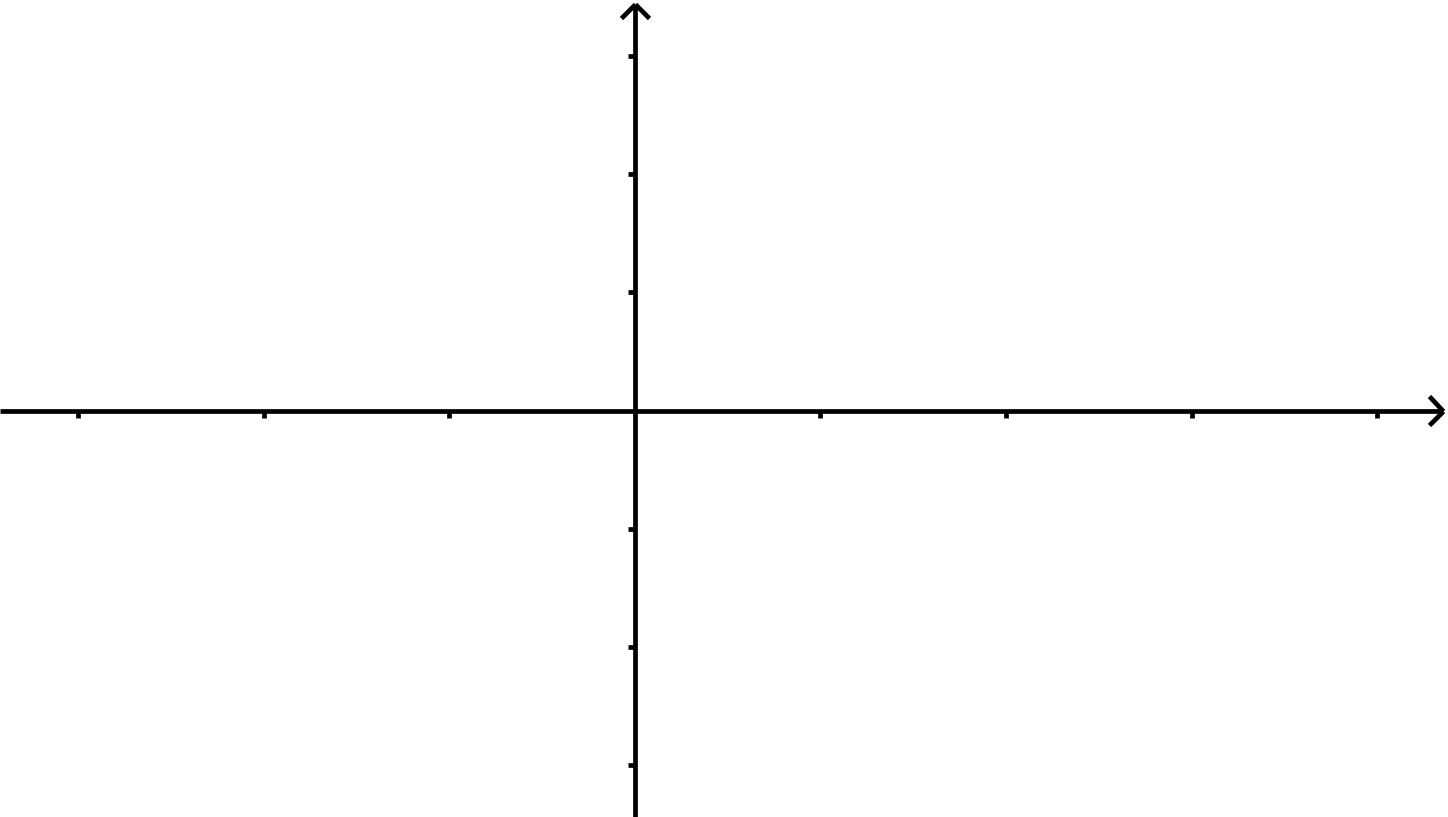
\includegraphics[scale=1.5]{gentrig1}}


\newpage

\item \begin{enumerate} \item Explain how to obtain the graph of $f(x)=3\cos(2x+\pi/2)$ from the graph of $y=\cos(x)$. \\[.75in]

\item Determine the period, amplitude, and phase shift.\\[1.5in]

\item Find an interval containing exactly one cycle.\vfill

\item Sketch the graph of $f(x)=3\cos(2x+\pi/2)$. 
\end{enumerate} 

\scalebox{.8}{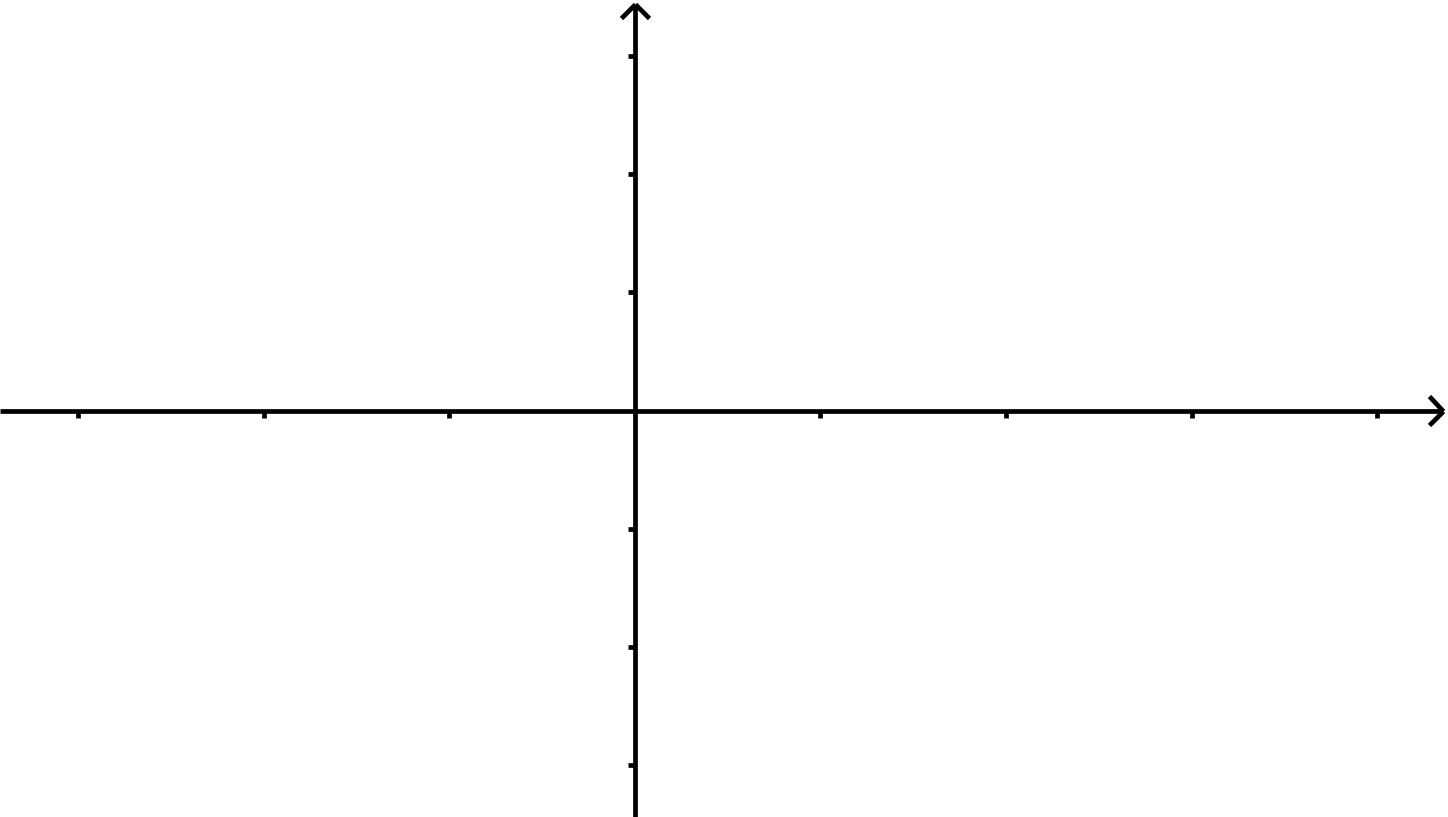
\includegraphics[scale=1.5]{gentrig1}}\\[.5in]



\newpage



\item Determine the period, amplitude, and phase shift of the function. \begin{enumerate}
\item $f(x)= -2 \sin(3x-7)$ \\[1in] 
%\item $g(x)= \cos\left(x+\dfrac{\pi}{7}\right)$ \\[.5in] 
\item $y = \cos\left(\dfrac{\pi x}{3}+\pi\right)$ \\[1in]
\end{enumerate}


\subsection{Determine a Formula for a Sine or Cosine Wave} ~

\item Express the equation for the sine wave shown below in the form
  $y=a\sin(bx+c)+d$. Then express the equation for the cosine wave
  shown below in the form $y=a\cos(bx+c)+d$.  In your equation, use
  $a>0$, $b>0$, and the least possible positive real number $c$.



 \begin{tikzpicture}[y=0.6cm, x=0.6cm,font=\sffamily]
    %% ticks
    \draw[step = 1, gray,dashed] (-1,-3) grid (8,7);
    %% axis
    \draw[thick,->] (-1.5,0) -- coordinate (x axis mid) (8.5,0) node[anchor = north west] {};
    \draw[thick,->] (0,-3.5) -- coordinate (y axis mid) (0,7.5) node[anchor = north east] {};
    \foreach \y in {-3,-2,-1,1,2,...,7} {
      \draw (1pt, \y) -- (-1pt, \y) node[yshift=-6,xshift=-1,anchor=east] {$\y$};
    }
    \foreach \x in {-1,1,2,...,8} {
      \draw (\x,1pt) -- (\x,-1pt) node[yshift=-5,xshift=-1,anchor=east] {$\x$};
    }

    \begin{scope}
      % \clip(-4,-1) rectangle (8,5);
%      \draw[scale=1.0,domain=-1:8,smooth,variable=\x,very thick,black,samples=120] 
%           plot ({\x},{2*cos(deg(pi*\x))-1}) node[anchor=west] {$f(x)$};
      \draw[scale=1.0,dotted,domain=-1:8,smooth,variable=\x,ultra thick,black,samples=120] 
          plot ({\x},{3*sin(deg(0.5*pi*\x-pi/4))+2}) node[anchor=west] {$f(x)$};
     \fill[black] (3/2,5) circle [radius=0.5ex] node[anchor=south west] {$\left(\frac{3}{2},5\right)$};
      \fill[black] (11/2,5) circle [radius=0.5ex] node[anchor=south west] {$\left(\frac{11}{2},5\right)$};
    \end{scope}

  \end{tikzpicture}



\vfill



%
%
%\newpage
%
%
%\subsection{Model Sinusoidal Behavior} ~
%
%
%\item The water level relative to the top of a boat dock varies with the tides.  One particular day, low tide occurs at midnight and the water level is 7ft below the dock.  The first high tide of the day occurs at approximately 6:00 AM, and the water level is 3ft below the dock.  The next low tide occurs at noon and the water level is again 7ft below the dock.\\
%
%Assuming that this pattern continues indefinitely and behaves like a cosine wave, write a function of the form $w(t)=A\cos(Bt+C)+D$.  The value $w(t)$ is the water level (in ft) relative to the top of the dock, $t$ hours after midnight.

\end{enumerate}
\vfill

\newpage
\noindent \textbf{Student Learning Outcomes Check}

\begin{enumerate}
\item Are you able to graph $a\sin(bx+c)$ and $a\cos(bx+c)$?
\item Can you determine a sine and cosine wave given a written description?
\item Can you determine the formula for a sine or cosine wave given the graph of the function?

\end{enumerate}

\noindent \textbf{If any of your answers were no, please ask about these topics in class.}


\actTitle{4.7 - Inverse Trigonometric Functions}

\videoLink{Section 4.7 day 1}{https://www.youtube.com/playlist?list=PLYHZK3b8UFw084fqUEZ7lpLyl4MJiCOwu}
%\videoLink{Section 4.7 day 2}{https://www.youtube.com/playlist?list=PLYHZK3b8UFw0JZy4oRGwxyv_LaTgWK5r2}


\noindent \textbf{Topics:}  inverse trig functions\\

\noindent \textbf{Student Learning Outcomes:}
\begin{enumerate}
\item Students will be able to evaluate the inverse trigonometric functions for sine, cosine, and tangent.
\item Students will be able to solve trigonometric equations using inverse trigonometric functions.
\item Students will be able to find the composition of trigonometric and inverse trigonometric functions.
\end{enumerate}

\hrule 

\bigskip

\noindent \underline{Recall:  } A one-to-one function has an inverse function.
\subsection{Evaluate the Inverse Sine Function}

Let's draw a graph of sine and find it's inverse function:
\vfill

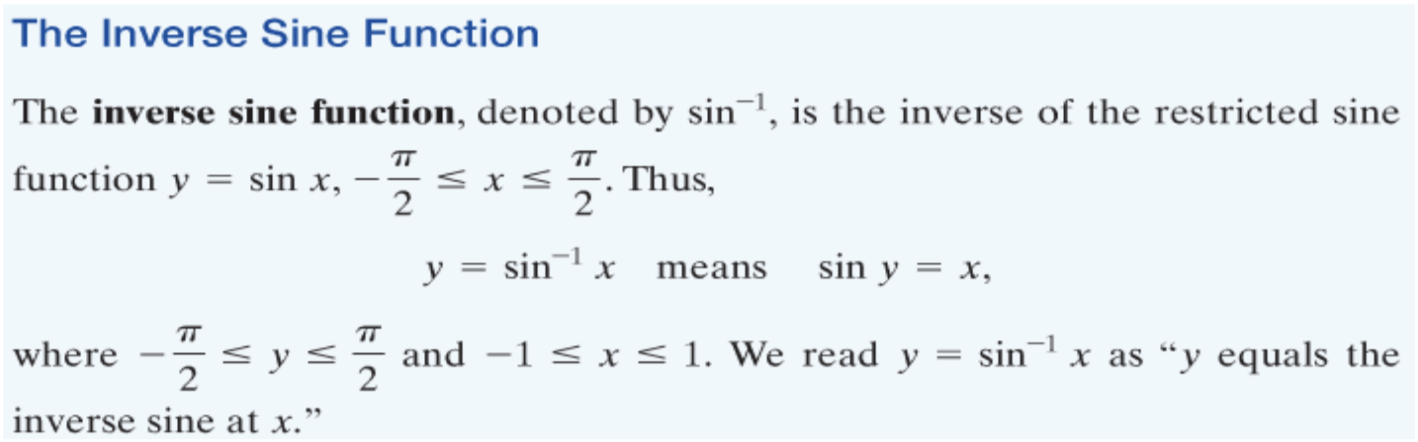
\includegraphics[scale=.7]{sineinverse}\\
\noindent Domain:\\[.5in]
\noindent Range:\\

\newpage
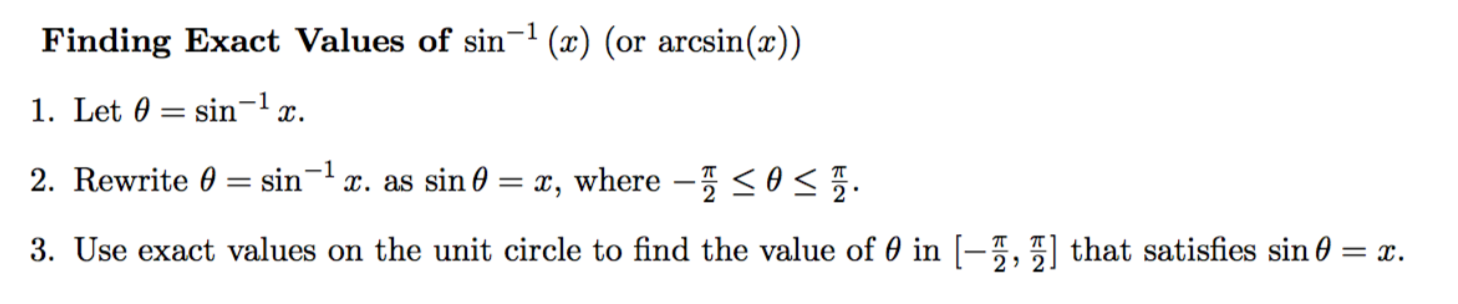
\includegraphics[scale=.7]{findingsineinverse}\\




\begin{enumerate}
\vspace{-.1in}
\item Find the exact values of an inverse function:

\begin{enumerate} 
\item $\displaystyle \sin^{-1}\left(\frac{1}{2}\right)=$\\[.5in]

\item $\displaystyle \sin^{-1}\left(\frac{\sqrt{3}}{2}\right)=$\\[.5in]

\item $\displaystyle \sin^{-1}\left(-\frac{1}{2}\right)=$\\[.5in]
\end{enumerate}




\subsection{Evaluate the Inverse Cosine Function}

Let's draw a graph of cosine and find it's inverse function:
\vfill

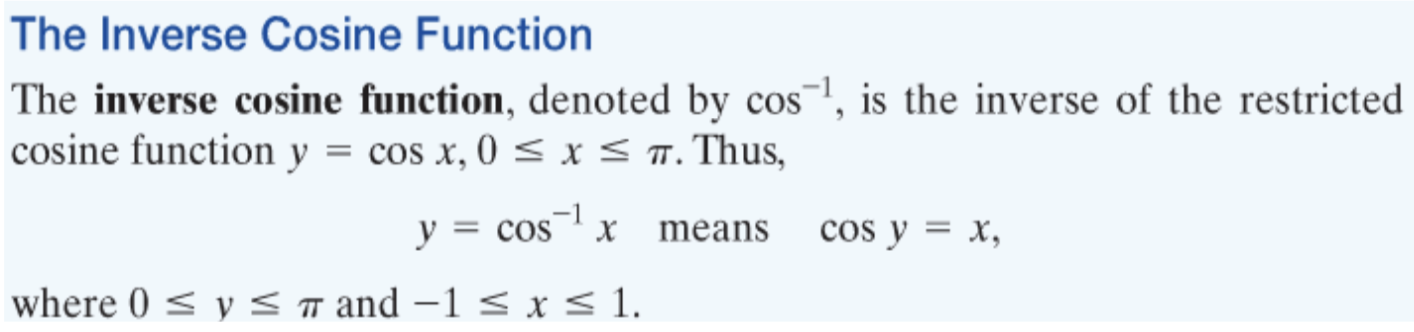
\includegraphics[scale=.7]{cosineinverse}\\
\noindent Domain:\\[.5in]
\noindent Range:\\

\newpage
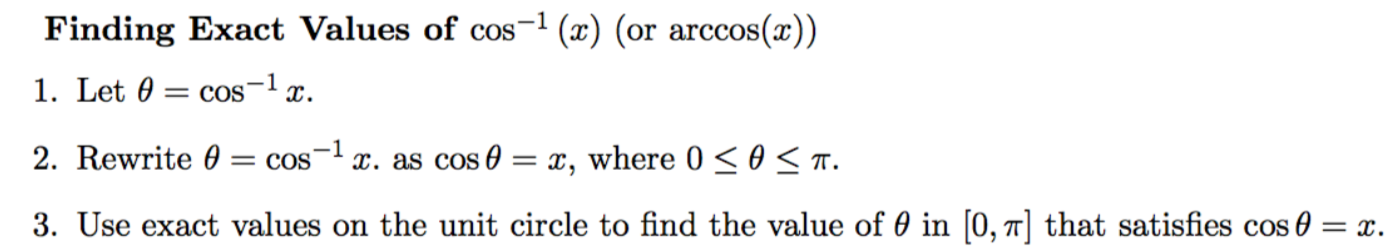
\includegraphics[scale=.7]{findingcosineinverse}\\




\vspace{-.1in}
\item Find the exact values of an inverse function:
 \begin{enumerate}
\item $\displaystyle \cos^{-1}\left(\frac{\sqrt{3}}{2}\right)=$\\[.5in]

\item $\displaystyle \cos^{-1}\left(-\frac{\sqrt{2}}{2}\right)=$\\[.5in]

\item $\displaystyle \cos^{-1}\left(\frac{1}{2}\right)=$\\[.5in]

\end{enumerate}




\subsection{Evaluate the Inverse Tangent Function}

Let's draw a graph of tangent and find it's inverse function:
\vfill

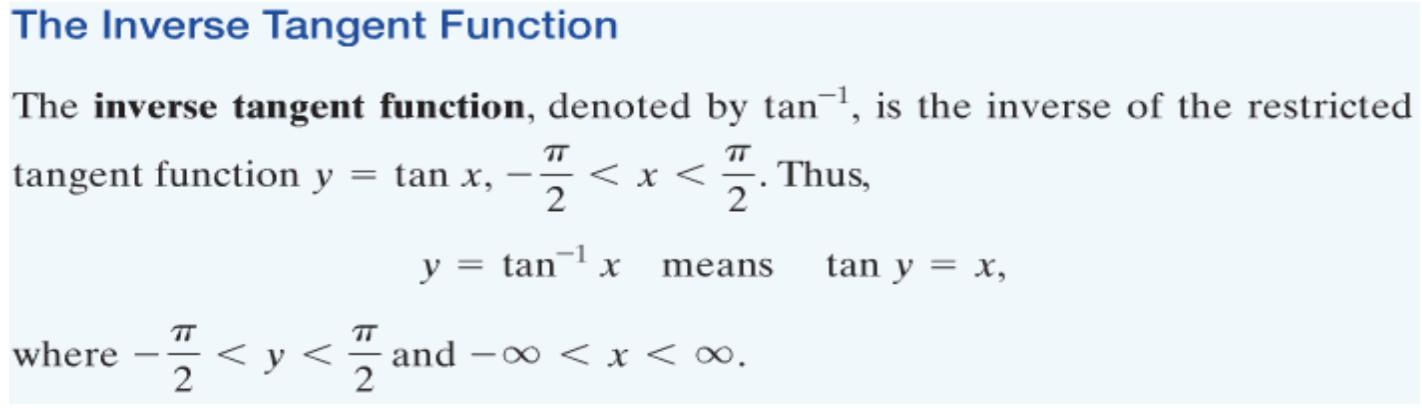
\includegraphics[scale=.7]{tangentinverse}\\
\noindent Domain:\\[.5in]
\noindent Range:\\

\newpage
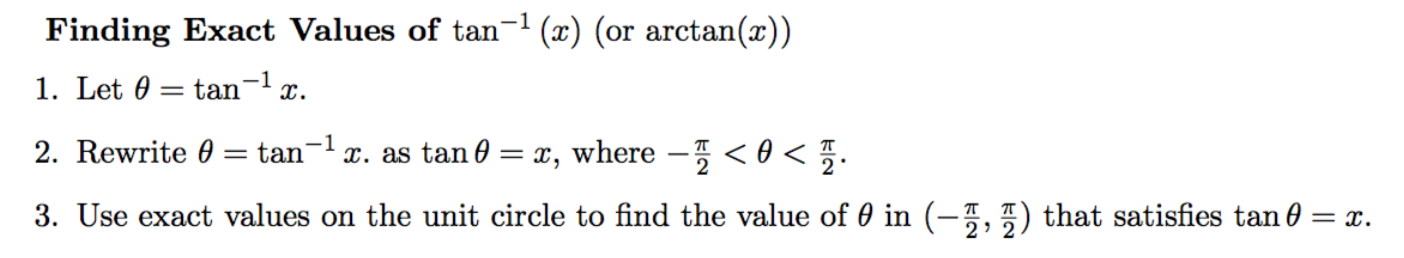
\includegraphics[scale=.7]{findingtangentinverse}\\




\vspace{-.1in}
\item Find the exact values of an inverse function:
 \begin{enumerate}
\item $\displaystyle \tan^{-1}\left(\frac{\sqrt{3}}{3}\right)=$\\[.5in]

\item $\displaystyle \tan^{-1}(0)=$\\[.5in]

\item $\displaystyle \tan^{-1}(1)=$\\[.5in]

\end{enumerate}


\subsection{Approximate Inverse Trigonometric Functions on a Calculator} ~

\item Use a calculator to find the value of each expression rounded to 2 decimal places in radians and degrees.
\begin{enumerate}
\item $\sin^{-1}(.7)=$\\
\item $\cos^{-1}(-.47)=$\\
\item $\tan^{-1}(-14)=$\\
\end{enumerate}


\newpage

\subsection{Inverse Properties of Trigonometric Functions} ~

\includegraphics[scale=.7]{inverseprops}

\item Find the exact value of the expression.  Do not use a calculator.
\begin{enumerate}
\item $\displaystyle \cos\left(\cos^{-1}(-0.4)\right)$\vfill
\item  $\displaystyle \sin^{-1}\left(\cos\left(\frac{\pi}{12}\right)\right)$\vfill
\item $\displaystyle \sin^{-1}\left(\sin\left(\frac{3\pi}{12}\right)\right)$\vfill
\newpage
\item $\displaystyle \tan\left(\tan^{-1}(11)\right)$\vfill
\item  $\displaystyle \tan^{-1}\left(\tan\left(-\frac{\pi}{4}\right)\right)$\vfill
\item  $\displaystyle \sin^{-1}\left(\sin(\pi)\right)$\vfill
\item $\displaystyle \sin\left(\sin^{-1}\left(\pi\right)\right)$\vfill
\end{enumerate}

\subsection{Composing Trigonometric and Inverse Trigonometric  Functions} ~

\item Use a sketch to find the exact value of each expression.
\begin{enumerate}
\item $\displaystyle \cos\left(\sin^{-1}\left(\frac{24}{26}\right)\right)$\vfill
\vfill
\newpage
\item $\displaystyle \tan\left(\cos^{-1}\left(-\frac{10}{26}\right)\right)$\vfill
\item $\displaystyle \sec\left(\sin^{-1}\left(-\frac{1}{6}\right)\right)$\vfill
\end{enumerate}


\end{enumerate}
\vfill
\noindent \textbf{Student Learning Outcomes Check}

\begin{enumerate}
\item Can you evaluate the inverse trigonometric functions for sine, cosine, and tangent?
\item Can you solve trigonometric equations using inverse trigonometric functions?
\item Are you able to find the composition of trigonometric and inverse trigonometric functions?

\end{enumerate}

\noindent \textbf{If any of your answers were no, please ask about these topics in class.}


\actTitle{5.1 - Fundamental Trigonometric Identities}

\noindent \textbf{Topics:}  inverse trig functions\\

\noindent \textbf{Student Learning Outcomes:}
\begin{enumerate}
\item Students will be able to simplify trigonometric expressions.
\item Students will be able to verify trigonometric identities.

\end{enumerate}

\hrule 

\bigskip

\subsection{Simplifying Trigonometric Expressions} ~

\begin{boxthm}
{\bf Fundamental Trigonometric Identities}

Reciprocal Identities

$$\sin(x) =\frac{1}{\csc(x)} \hspace{2cm}\cos(x) = \frac{1}{\sec(x)}\hspace{2cm}\tan(x) = \frac{1}{\cot(x)}$$

$$\csc(x) =\frac{1}{\sin(x)} \hspace{2cm}\sec(x) = \frac{1}{\cos(x)}\hspace{2cm}\cot(x) = \frac{1}{\tan(x)}$$

Quotient Identities

$$\tan(x) = \frac{\sin(x)}{\cos(x)} \hspace{3cm} \cot(x) = \frac{\cos(x)}{\sin(x)}$$

Pythagorean Identities

$$\sin^2(x) + \cos^2(x)=1 \hspace{2cm}\tan^2(x) +1 = \sec^2(x) \hspace{2cm}1+\cot^2(x) = \csc^2(x)$$

Even and Odd Identities

$$\sin( -x) =-\sin(x)\hspace{2cm}\cos( -x) = \cos(x)\hspace{2cm}\tan(- x) = -\tan(x)$$

$$\csc( -x) =-\csc(x)\hspace{2cm}\sec( -x) = \sec(x)\hspace{2cm}\cot(- x) = -\cot(x)$$

\end{boxthm}

{\bf Note:} It is often helpful to notice alternative forms of
Pythagorean Identities, such as $\sin^2(x) = 1-\cos^2(x)$ or
$\cos^2(x) = 1-\sin^2(x)$.




\begin{enumerate}
\vspace{-.1in}
\item Simplify each of the following. Write the final form with no fractions or products.

\begin{enumerate}
\item $\tan(x) \cos^2(x) \sec(x)$
\vfill


\newpage

\item $\displaystyle \frac{\cos (\theta)}{1+\sin (\theta)}+\tan (\theta)$
\vfill

%\item $\displaystyle \frac{\tan^2 (t) - 1}{\tan (t) \sin( t) + \sin (t)}$
%\vfill

\end{enumerate}

\subsection{Verify Trigonometric Identities} ~

\begin{boxthm}
{\bf Trigonometric Identities}

An {\bf identity} is an equation which it is true for all values of x for which the expressions on the left and right are defined.

\vspace{0.5cm}

{\bf Guidelines for proving Trigonometric Identities:}
\begin{enumerate}
\item Work with one side of the equation (usually the more complicated side) and keep the other side in mind as your final goal.

\item Look for opportunities to apply the fundamental identities.

\begin{itemize}

\item If the expression is a product or quotient of factors, consider the reciprocal and quotient identities.

\item If squared terms are present, look to see if the terms can be grouped in one of the forms of a Pythagorean identity.

\item If an expression involves a negative argument, consider using the even or odd function identities.

\end{itemize}

\item Apply basic algebraic techniques such as factoring, multiplying terms, combining like terms, and writing fractions with a common denominator.

\item Consider writing expressions explicitly in terms of sine and cosine.

\end{enumerate}

\end{boxthm}

\newpage

\item Prove that each of the following equations is an identity. (Note: The {\bf entire} proof is your answer.)
\begin{enumerate}
\item $\displaystyle \frac{\sin(-x)\cot(-x)}{\cos(x)} = 1$
\vfill

\item $\displaystyle \frac{1}{1-\cos (x)}-\frac{1}{1+\cos (x)} = 2\cot (x)\csc (x)$
\vfill
\vfill
\newpage

\item $\displaystyle 1 - \frac{\sin^2(t)}{1+\cos(t)} = \cos(t)$
\vfill

\item $\displaystyle \frac{\cot(x)}{\csc(x)}-\frac{\csc(x)}{\cot(x)} = -\sin(x) \tan(x)$
\vfill

\newpage

%\item $\displaystyle \frac{1}{1+\sin(x)}+\frac{1}{1-\sin(x)} = 2\sec^2(x)$
%\vfill

\item $\displaystyle \frac{\sin(x)}{\csc(x) - \cot(x)} = 1+\cos(x)$
\vfill


\end{enumerate}


\end{enumerate}
\vfill
\noindent \textbf{Student Learning Outcomes Check}

\begin{enumerate}
\item Are you able to simplify trigonometric expressions?
\item Are you able to verify trigonometric identities?

\end{enumerate}

\noindent \textbf{If any of your answers were no, please ask about these topics in class.}


\actTitle{5.2 - Sum and Difference Formulas}

\videoLink{Section 5.2}{https://www.youtube.com/playlist?list=PLYHZK3b8UFw3NgZa9wBc8k8LS5w45veeB}

\noindent \textbf{Topics:}  sum and difference formulas\\

\noindent \textbf{Student Learning Outcomes:}
\begin{enumerate}
\item Students will be able apply the sum and difference formulas for sine and cosine.
\item Students will be able to apply the sum and difference formulas for tangent.
\item Students will be able to use sum and difference formulas to verify identities.

\end{enumerate}

\hrule 

\bigskip

\subsection{Apply the Sum and Difference Formulas} ~

\begin{boxthm}
{\bf Sum and Difference Identities}

$$\sin(u+v) = \sin(u) \cos(v) + \cos(u) \sin(v) \hspace{1cm}\sin(u-v) = \sin(u) \cos(v) - \cos(u) \sin(v)$$

$$\cos(u+v) = \cos(u)\cos(v) - \sin(u)\sin(v) \hspace{1cm}\cos(u-v) = \cos(u) \cos(v) + \sin(u) \sin(v)$$

$$\tan(u+v) = \frac{\tan(u) +\tan(v)}{1-\tan(u) \tan(v)} \hspace{1cm}\tan(u-v) =  \frac{\tan(u) -\tan(v)}{1-\tan(u) \tan(v)}$$

\end{boxthm}






\begin{enumerate}
\vspace{-.1in}
\item Evaluate each of the following using the above identities and the unit circle.


\begin{enumerate}
\item $\cos\left(15^{\circ}\right)$
\vfill

\item $\sin\left(\frac{5\pi}{12}\right)$
\vfill

\newpage

\item $\sin\left(25^{\circ}\right)\cos\left(35^{\circ}\right) +\cos\left(25^{\circ}\right)\sin\left(35^{\circ}\right)$
\vfill

\item $\tan\left(75^{\circ}\right)$
\vfill

\item $\sin\left(\frac{\pi}{12}\right)$
\vfill
 
\item $\cos\left(99^{\circ}\right)\cos\left(36^{\circ}\right)-\sin\left(99^{\circ}\right)\sin\left(36^{\circ}\right)$
\vfill

\end{enumerate}

\newpage


%\item Find the exact value of $\cos (\alpha - \beta)$ given that $\sin\left(\alpha\right) = -\frac{4}{5}$ and $\cos\left(\beta\right) = -\frac{5}{8}$ for $\alpha$ in Quadrant III and $\beta$ in Quadrant II.
%\vfill

\item Find the exact value of $\sin(\alpha + \beta)$ given that $\sin\left(\alpha\right) = \frac{5}{13}$ and $\cos\left(\beta\right) = \frac{5}{6}$ for $\alpha$ in Quadrant II and $\beta$ in Quadrant IV.
\vfill



\item Find the exact value of each of the following.

$$\sin \left( \arctan \left(-\frac{9}{4}\right)+\arccos \left(\frac{8}{17}\right)\right)$$
\vfill

%\item $\cos \left( \arcsin \left(-\frac{12}{37}\right)+\arctan \left(\frac{5}{12}\right)\right)$
%\vfill


\newpage

\subsection{Use Sum and Difference Formulas to Verify Identitities} ~

\item Prove that each of the following is an identity.

\begin{enumerate}
\item $\sin \left(\frac{\pi}{2}-x\right)=\cos(x)$
\vfill

\item $\sin(x+y)-\sin(x-y) = 2 \cos\left(x\right) \sin(y)$
\vfill

\item $\tan(\pi-x)=-\tan(x)$
\vfill


\end{enumerate}



\end{enumerate}

\noindent \textbf{Student Learning Outcomes Check}

\begin{enumerate}
\item Can you apply the sum and difference formulas for sine and cosine?
\item Can you apply the sum and difference formulas for tangent?
\item Are you able to use sum and difference formulas to verify identities?
\end{enumerate}

\noindent \textbf{If any of your answers were no, please ask about these topics in class.}




\chapter{GNU Free Documentation License}

\hfuzz = .6pt % avoid black boxes
           
%---------------------------------------------------------------------
%\chapter*{\rlap{GNU Free Documentation License}}
%\phantomsection  % so hyperref creates bookmarks
%\addcontentsline{toc}{chapter}{GNU Free Documentation License}
%\label{label_fdl}

 \begin{center}

       Version 1.3, 3 November 2008


 Copyright \copyright{} 2000, 2001, 2002, 2007, 2008  Free Software Foundation, Inc.
 
 \bigskip
 
     \texttt{<http://fsf.org/>}
  
 \bigskip
 
 Everyone is permitted to copy and distribute verbatim copies
 of this license document, but changing it is not allowed.
\end{center}


%\begin{center}
\noindent
{\bf\normalsize Preamble}
%\end{center}

The purpose of this License is to make a manual, textbook, or other
functional and useful document ``free'' in the sense of freedom: to
assure everyone the effective freedom to copy and redistribute it,
with or without modifying it, either commercially or noncommercially.
Secondarily, this License preserves for the author and publisher a way
to get credit for their work, while not being considered responsible
for modifications made by others.

This License is a kind of ``copyleft'', which means that derivative
works of the document must themselves be free in the same sense.  It
complements the GNU General Public License, which is a copyleft
license designed for free software.

We have designed this License in order to use it for manuals for free
software, because free software needs free documentation: a free
program should come with manuals providing the same freedoms that the
software does.  But this License is not limited to software manuals;
it can be used for any textual work, regardless of subject matter or
whether it is published as a printed book.  We recommend this License
principally for works whose purpose is instruction or reference.


%\begin{center}
\noindent
{\normalsize\bf 1. APPLICABILITY AND DEFINITIONS\par}
%\phantomsection
%\addcontentsline{toc}{section}{1. APPLICABILITY AND DEFINITIONS}
%\end{center}

This License applies to any manual or other work, in any medium, that
contains a notice placed by the copyright holder saying it can be
distributed under the terms of this License.  Such a notice grants a
world-wide, royalty-free license, unlimited in duration, to use that
work under the conditions stated herein.  The ``\textbf{Document}'', below,
refers to any such manual or work.  Any member of the public is a
licensee, and is addressed as ``\textbf{you}''.  You accept the license if you
copy, modify or distribute the work in a way requiring permission
under copyright law.

A ``\textbf{Modified Version}'' of the Document means any work containing the
Document or a portion of it, either copied verbatim, or with
modifications and/or translated into another language.

A ``\textbf{Secondary Section}'' is a named appendix or a front-matter section of
the Document that deals exclusively with the relationship of the
publishers or authors of the Document to the Document's overall subject
(or to related matters) and contains nothing that could fall directly
within that overall subject.  (Thus, if the Document is in part a
textbook of mathematics, a Secondary Section may not explain any
mathematics.)  The relationship could be a matter of historical
connection with the subject or with related matters, or of legal,
commercial, philosophical, ethical or political position regarding
them.

The ``\textbf{Invariant Sections}'' are certain Secondary Sections whose titles
are designated, as being those of Invariant Sections, in the notice
that says that the Document is released under this License.  If a
section does not fit the above definition of Secondary then it is not
allowed to be designated as Invariant.  The Document may contain zero
Invariant Sections.  If the Document does not identify any Invariant
Sections then there are none.

The ``\textbf{Cover Texts}'' are certain short passages of text that are listed,
as Front-Cover Texts or Back-Cover Texts, in the notice that says that
the Document is released under this License.  A Front-Cover Text may
be at most 5 words, and a Back-Cover Text may be at most 25 words.

A ``\textbf{Transparent}'' copy of the Document means a machine-readable copy,
represented in a format whose specification is available to the
general public, that is suitable for revising the document
straightforwardly with generic text editors or (for images composed of
pixels) generic paint programs or (for drawings) some widely available
drawing editor, and that is suitable for input to text formatters or
for automatic translation to a variety of formats suitable for input
to text formatters.  A copy made in an otherwise Transparent file
format whose markup, or absence of markup, has been arranged to thwart
or discourage subsequent modification by readers is not Transparent.
An image format is not Transparent if used for any substantial amount
of text.  A copy that is not ``Transparent'' is called ``\textbf{Opaque}''.

Examples of suitable formats for Transparent copies include plain
ASCII without markup, Texinfo input format, LaTeX input format, SGML
or XML using a publicly available DTD, and standard-conforming simple
HTML, PostScript or PDF designed for human modification.  Examples of
transparent image formats include PNG, XCF and JPG.  Opaque formats
include proprietary formats that can be read and edited only by
proprietary word processors, SGML or XML for which the DTD and/or
processing tools are not generally available, and the
machine-generated HTML, PostScript or PDF produced by some word
processors for output purposes only.

The ``\textbf{Title Page}'' means, for a printed book, the title page itself,
plus such following pages as are needed to hold, legibly, the material
this License requires to appear in the title page.  For works in
formats which do not have any title page as such, ``Title Page'' means
the text near the most prominent appearance of the work's title,
preceding the beginning of the body of the text.

The ``\textbf{publisher}'' means any person or entity that distributes
copies of the Document to the public.

A section ``\textbf{Entitled XYZ}'' means a named subunit of the Document whose
title either is precisely XYZ or contains XYZ in parentheses following
text that translates XYZ in another language.  (Here XYZ stands for a
specific section name mentioned below, such as ``\textbf{Acknowledgements}'',
``\textbf{Dedications}'', ``\textbf{Endorsements}'', or ``\textbf{History}''.)  
To ``\textbf{Preserve the Title}''
of such a section when you modify the Document means that it remains a
section ``Entitled XYZ'' according to this definition.

The Document may include Warranty Disclaimers next to the notice which
states that this License applies to the Document.  These Warranty
Disclaimers are considered to be included by reference in this
License, but only as regards disclaiming warranties: any other
implication that these Warranty Disclaimers may have is void and has
no effect on the meaning of this License.


%\begin{center}
\noindent
{\normalsize\bf 2. VERBATIM COPYING\par}
%\phantomsection
%\addcontentsline{toc}{section}{2. VERBATIM COPYING}
%\end{center}

You may copy and distribute the Document in any medium, either
commercially or noncommercially, provided that this License, the
copyright notices, and the license notice saying this License applies
to the Document are reproduced in all copies, and that you add no other
conditions whatsoever to those of this License.  You may not use
technical measures to obstruct or control the reading or further
copying of the copies you make or distribute.  However, you may accept
compensation in exchange for copies.  If you distribute a large enough
number of copies you must also follow the conditions in section~3.

You may also lend copies, under the same conditions stated above, and
you may publicly display copies.


%\begin{center}
\noindent
{\normalsize\bf 3. COPYING IN QUANTITY\par}
%\phantomsection
%\addcontentsline{toc}{section}{3. COPYING IN QUANTITY}
%\end{center}


If you publish printed copies (or copies in media that commonly have
printed covers) of the Document, numbering more than 100, and the
Document's license notice requires Cover Texts, you must enclose the
copies in covers that carry, clearly and legibly, all these Cover
Texts: Front-Cover Texts on the front cover, and Back-Cover Texts on
the back cover.  Both covers must also clearly and legibly identify
you as the publisher of these copies.  The front cover must present
the full title with all words of the title equally prominent and
visible.  You may add other material on the covers in addition.
Copying with changes limited to the covers, as long as they preserve
the title of the Document and satisfy these conditions, can be treated
as verbatim copying in other respects.

If the required texts for either cover are too voluminous to fit
legibly, you should put the first ones listed (as many as fit
reasonably) on the actual cover, and continue the rest onto adjacent
pages.

If you publish or distribute Opaque copies of the Document numbering
more than 100, you must either include a machine-readable Transparent
copy along with each Opaque copy, or state in or with each Opaque copy
a computer-network location from which the general network-using
public has access to download using public-standard network protocols
a complete Transparent copy of the Document, free of added material.
If you use the latter option, you must take reasonably prudent steps,
when you begin distribution of Opaque copies in quantity, to ensure
that this Transparent copy will remain thus accessible at the stated
location until at least one year after the last time you distribute an
Opaque copy (directly or through your agents or retailers) of that
edition to the public.

It is requested, but not required, that you contact the authors of the
Document well before redistributing any large number of copies, to give
them a chance to provide you with an updated version of the Document.


%\begin{center}
\noindent
{\normalsize\bf 4. MODIFICATIONS\par}
%\phantomsection
%\addcontentsline{toc}{section}{4. MODIFICATIONS}
%\end{center}

You may copy and distribute a Modified Version of the Document under
the conditions of sections 2 and 3 above, provided that you release
the Modified Version under precisely this License, with the Modified
Version filling the role of the Document, thus licensing distribution
and modification of the Modified Version to whoever possesses a copy
of it.  In addition, you must do these things in the Modified Version:

\begin{itemize}
\item[A.] 
   Use in the Title Page (and on the covers, if any) a title distinct
   from that of the Document, and from those of previous versions
   (which should, if there were any, be listed in the History section
   of the Document).  You may use the same title as a previous version
   if the original publisher of that version gives permission.
   
\item[B.]
   List on the Title Page, as authors, one or more persons or entities
   responsible for authorship of the modifications in the Modified
   Version, together with at least five of the principal authors of the
   Document (all of its principal authors, if it has fewer than five),
   unless they release you from this requirement.
   
\item[C.]
   State on the Title page the name of the publisher of the
   Modified Version, as the publisher.
   
\item[D.]
   Preserve all the copyright notices of the Document.
   
\item[E.]
   Add an appropriate copyright notice for your modifications
   adjacent to the other copyright notices.
   
\item[F.]
   Include, immediately after the copyright notices, a license notice
   giving the public permission to use the Modified Version under the
   terms of this License, in the form shown in the Addendum below.
   
\item[G.]
   Preserve in that license notice the full lists of Invariant Sections
   and required Cover Texts given in the Document's license notice.
   
\item[H.]
   Include an unaltered copy of this License.
   
\item[I.]
   Preserve the section Entitled ``History'', Preserve its Title, and add
   to it an item stating at least the title, year, new authors, and
   publisher of the Modified Version as given on the Title Page.  If
   there is no section Entitled ``History'' in the Document, create one
   stating the title, year, authors, and publisher of the Document as
   given on its Title Page, then add an item describing the Modified
   Version as stated in the previous sentence.
   
\item[J.]
   Preserve the network location, if any, given in the Document for
   public access to a Transparent copy of the Document, and likewise
   the network locations given in the Document for previous versions
   it was based on.  These may be placed in the ``History'' section.
   You may omit a network location for a work that was published at
   least four years before the Document itself, or if the original
   publisher of the version it refers to gives permission.
   
\item[K.]
   For any section Entitled ``Acknowledgements'' or ``Dedications'',
   Preserve the Title of the section, and preserve in the section all
   the substance and tone of each of the contributor acknowledgements
   and/or dedications given therein.
   
\item[L.]
   Preserve all the Invariant Sections of the Document,
   unaltered in their text and in their titles.  Section numbers
   or the equivalent are not considered part of the section titles.
   
\item[M.]
   Delete any section Entitled ``Endorsements''.  Such a section
   may not be included in the Modified Version.
   
\item[N.]
   Do not retitle any existing section to be Entitled ``Endorsements''
   or to conflict in title with any Invariant Section.
   
\item[O.]
   Preserve any Warranty Disclaimers.
\end{itemize}

If the Modified Version includes new front-matter sections or
appendices that qualify as Secondary Sections and contain no material
copied from the Document, you may at your option designate some or all
of these sections as invariant.  To do this, add their titles to the
list of Invariant Sections in the Modified Version's license notice.
These titles must be distinct from any other section titles.

You may add a section Entitled ``Endorsements'', provided it contains
nothing but endorsements of your Modified Version by various
parties---for example, statements of peer review or that the text has
been approved by an organization as the authoritative definition of a
standard.

You may add a passage of up to five words as a Front-Cover Text, and a
passage of up to 25 words as a Back-Cover Text, to the end of the list
of Cover Texts in the Modified Version.  Only one passage of
Front-Cover Text and one of Back-Cover Text may be added by (or
through arrangements made by) any one entity.  If the Document already
includes a cover text for the same cover, previously added by you or
by arrangement made by the same entity you are acting on behalf of,
you may not add another; but you may replace the old one, on explicit
permission from the previous publisher that added the old one.

The author(s) and publisher(s) of the Document do not by this License
give permission to use their names for publicity for or to assert or
imply endorsement of any Modified Version.


%\begin{center}
\noindent
{\normalsize\bf 5. COMBINING DOCUMENTS\par}
%\phantomsection
%\addcontentsline{toc}{section}{5. COMBINING DOCUMENTS}
%\end{center}


You may combine the Document with other documents released under this
License, under the terms defined in section~4 above for modified
versions, provided that you include in the combination all of the
Invariant Sections of all of the original documents, unmodified, and
list them all as Invariant Sections of your combined work in its
license notice, and that you preserve all their Warranty Disclaimers.

The combined work need only contain one copy of this License, and
multiple identical Invariant Sections may be replaced with a single
copy.  If there are multiple Invariant Sections with the same name but
different contents, make the title of each such section unique by
adding at the end of it, in parentheses, the name of the original
author or publisher of that section if known, or else a unique number.
Make the same adjustment to the section titles in the list of
Invariant Sections in the license notice of the combined work.

In the combination, you must combine any sections Entitled ``History''
in the various original documents, forming one section Entitled
``History''; likewise combine any sections Entitled ``Acknowledgements'',
and any sections Entitled ``Dedications''.  You must delete all sections
Entitled ``Endorsements''.

%\begin{center}
\noindent
{\normalsize\bf 6. COLLECTIONS OF DOCUMENTS\par}
%\phantomsection
%\addcontentsline{toc}{section}{6. COLLECTIONS OF DOCUMENTS}
%\end{center}

You may make a collection consisting of the Document and other documents
released under this License, and replace the individual copies of this
License in the various documents with a single copy that is included in
the collection, provided that you follow the rules of this License for
verbatim copying of each of the documents in all other respects.

You may extract a single document from such a collection, and distribute
it individually under this License, provided you insert a copy of this
License into the extracted document, and follow this License in all
other respects regarding verbatim copying of that document.


%\begin{center}
\noindent
{\normalsize\bf 7. AGGREGATION WITH INDEPENDENT WORKS\par}
%\phantomsection
%\addcontentsline{toc}{section}{7. AGGREGATION WITH INDEPENDENT WORKS}
%\end{center}


A compilation of the Document or its derivatives with other separate
and independent documents or works, in or on a volume of a storage or
distribution medium, is called an ``aggregate'' if the copyright
resulting from the compilation is not used to limit the legal rights
of the compilation's users beyond what the individual works permit.
When the Document is included in an aggregate, this License does not
apply to the other works in the aggregate which are not themselves
derivative works of the Document.

If the Cover Text requirement of section~3 is applicable to these
copies of the Document, then if the Document is less than one half of
the entire aggregate, the Document's Cover Texts may be placed on
covers that bracket the Document within the aggregate, or the
electronic equivalent of covers if the Document is in electronic form.
Otherwise they must appear on printed covers that bracket the whole
aggregate.


%\begin{center}
\noindent
{\normalsize\bf 8. TRANSLATION\par}
%\phantomsection
%\addcontentsline{toc}{section}{8. TRANSLATION}
%\end{center}


Translation is considered a kind of modification, so you may
distribute translations of the Document under the terms of section~4.
Replacing Invariant Sections with translations requires special
permission from their copyright holders, but you may include
translations of some or all Invariant Sections in addition to the
original versions of these Invariant Sections.  You may include a
translation of this License, and all the license notices in the
Document, and any Warranty Disclaimers, provided that you also include
the original English version of this License and the original versions
of those notices and disclaimers.  In case of a disagreement between
the translation and the original version of this License or a notice
or disclaimer, the original version will prevail.

If a section in the Document is Entitled ``Acknowledgements'',
``Dedications'', or ``History'', the requirement (section~4) to Preserve
its Title (section~1) will typically require changing the actual
title.


%\begin{center}
\noindent
{\normalsize\bf 9. TERMINATION\par}
%\phantomsection
%\addcontentsline{toc}{section}{9. TERMINATION}
%\end{center}


You may not copy, modify, sublicense, or distribute the Document
except as expressly provided under this License.  Any attempt
otherwise to copy, modify, sublicense, or distribute it is void, and
will automatically terminate your rights under this License.

However, if you cease all violation of this License, then your license
from a particular copyright holder is reinstated (a) provisionally,
unless and until the copyright holder explicitly and finally
terminates your license, and (b) permanently, if the copyright holder
fails to notify you of the violation by some reasonable means prior to
60 days after the cessation.

Moreover, your license from a particular copyright holder is
reinstated permanently if the copyright holder notifies you of the
violation by some reasonable means, this is the first time you have
received notice of violation of this License (for any work) from that
copyright holder, and you cure the violation prior to 30 days after
your receipt of the notice.

Termination of your rights under this section does not terminate the
licenses of parties who have received copies or rights from you under
this License.  If your rights have been terminated and not permanently
reinstated, receipt of a copy of some or all of the same material does
not give you any rights to use it.


%\begin{center}
\noindent
{\normalsize\bf 10. FUTURE REVISIONS OF THIS LICENSE\par}
%\phantomsection
%\addcontentsline{toc}{section}{10. FUTURE REVISIONS OF THIS LICENSE}
%\end{center}


The Free Software Foundation may publish new, revised versions
of the GNU Free Documentation License from time to time.  Such new
versions will be similar in spirit to the present version, but may
differ in detail to address new problems or concerns.  See
\texttt{http://www.gnu.org/copyleft/}.

Each version of the License is given a distinguishing version number.
If the Document specifies that a particular numbered version of this
License ``or any later version'' applies to it, you have the option of
following the terms and conditions either of that specified version or
of any later version that has been published (not as a draft) by the
Free Software Foundation.  If the Document does not specify a version
number of this License, you may choose any version ever published (not
as a draft) by the Free Software Foundation.  If the Document
specifies that a proxy can decide which future versions of this
License can be used, that proxy's public statement of acceptance of a
version permanently authorizes you to choose that version for the
Document.


%\begin{center}
\noindent
{\normalsize\bf 11. RELICENSING\par}
%\phantomsection
%\addcontentsline{toc}{section}{11. RELICENSING}
%\end{center}


``Massive Multiauthor Collaboration Site'' (or ``MMC Site'') means any
World Wide Web server that publishes copyrightable works and also
provides prominent facilities for anybody to edit those works.  A
public wiki that anybody can edit is an example of such a server.  A
``Massive Multiauthor Collaboration'' (or ``MMC'') contained in the
site means any set of copyrightable works thus published on the MMC
site.

``CC-BY-SA'' means the Creative Commons Attribution-Share Alike 3.0
license published by Creative Commons Corporation, a not-for-profit
corporation with a principal place of business in San Francisco,
California, as well as future copyleft versions of that license
published by that same organization.

``Incorporate'' means to publish or republish a Document, in whole or
in part, as part of another Document.

An MMC is ``eligible for relicensing'' if it is licensed under this
License, and if all works that were first published under this License
somewhere other than this MMC, and subsequently incorporated in whole
or in part into the MMC, (1) had no cover texts or invariant sections,
and (2) were thus incorporated prior to November 1, 2008.

The operator of an MMC Site may republish an MMC contained in the site
under CC-BY-SA on the same site at any time before August 1, 2009,
provided the MMC is eligible for relicensing.


%\begin{center}
\noindent
{\normalsize\bf ADDENDUM: How to use this License for your documents\par}
%\phantomsection
%\addcontentsline{toc}{section}{ADDENDUM: How to use this License for your documents}
%\end{center}

To use this License in a document you have written, include a copy of
the License in the document and put the following copyright and
license notices just after the title page:

\bigskip
\begin{quote}
    Copyright \copyright{}  YEAR  YOUR NAME.
    Permission is granted to copy, distribute and/or modify this document
    under the terms of the GNU Free Documentation License, Version 1.3
    or any later version published by the Free Software Foundation;
    with no Invariant Sections, no Front-Cover Texts, and no Back-Cover Texts.
    A copy of the license is included in the section entitled ``GNU
    Free Documentation License''.
\end{quote}
\bigskip
    
If you have Invariant Sections, Front-Cover Texts and Back-Cover Texts,
replace the ``with \dots\ Texts.''\ line with this:

\bigskip
\begin{quote}
    with the Invariant Sections being LIST THEIR TITLES, with the
    Front-Cover Texts being LIST, and with the Back-Cover Texts being LIST.
\end{quote}
\bigskip
    
If you have Invariant Sections without Cover Texts, or some other
combination of the three, merge those two alternatives to suit the
situation.

If your document contains nontrivial examples of program code, we
recommend releasing these examples in parallel under your choice of
free software license, such as the GNU General Public License,
to permit their use in free software.

%---------------------------------------------------------------------


\end{document}
